%%%%%%%%%%%%%%
%% Run LaTeX on this file several times to get Table of Contents,
%% cross-references, and citations.

%% If you have font problems, you may edit the w-bookps.sty file
%% to customize the font names to match those on your system.

%% w-bksamp.tex. Current Version: Feb 16, 2012
%%%%%%%%%%%%%%%%%%%%%%%%%%%%%%%%%%%%%%%%%%%%%%%%%%%%%%%%%%%%%%%%
%
%  Sample file for
%  Wiley Book Style, Design No.: SD 001B, 7x10
%  Wiley Book Style, Design No.: SD 004B, 6x9
%
%
%  Prepared by Amy Hendrickson, TeXnology Inc.
%  http://www.texnology.com
%%%%%%%%%%%%%%%%%%%%%%%%%%%%%%%%%%%%%%%%%%%%%%%%%%%%%%%%%%%%%%%%

%%%%%%%%%%%%%
% 7x10
%\documentclass{wileySev}

% 6x9
\documentclass{wileySix}
\UseRawInputEncoding
\usepackage{graphicx}
\usepackage{listings}

\usepackage{color}

 
\definecolor{codegreen}{rgb}{0,0.6,0}
\definecolor{codegray}{rgb}{0.5,0.5,0.5}
\definecolor{codepurple}{rgb}{0.58,0,0.82}
\definecolor{backcolour}{rgb}{0.95,0.95,0.92}
 
\lstdefinestyle{mystyle}{
    backgroundcolor=\color{backcolour},   
    commentstyle=\color{codegreen},
    keywordstyle=\color{magenta},
    numberstyle=\tiny\color{codegray},
    stringstyle=\color{codepurple},
    basicstyle=\footnotesize,
    breakatwhitespace=false,         
    breaklines=true,                 
    captionpos=b,                    
    keepspaces=true,                 
    numbers=left,                    
    numbersep=5pt,                  
    showspaces=false,                
    showstringspaces=false,
    showtabs=false,                  
    tabsize=2,
    language=sh
}
 
\lstset{style=mystyle}

%%%%%%%
%% for times math: However, this package disables bold math (!)
%% \mathbf{x} will still work, but you will not have bold math
%% in section heads or chapter titles. If you don't use math
%% in those environments, mathptmx might be a good choice.

% \usepackage{mathptmx}

% For PostScript text
\usepackage{w-bookps}

%%%%%%%%%%%%%%%%%%%%%%%%%%%%%%%%%%%%%%%%%%%%%%%%%%%%%%%%%%%%%%%%
%% Other packages you might want to use:

% for chapter bibliography made with BibTeX
% \usepackage{chapterbib}

% for multiple indices
% \usepackage{multind}

% for answers to problems
% \usepackage{answers}

%%%%%%%%%%%%%%%%%%%%%%%%%%%%%%
%% Change options here if you want:
%%
%% How many levels of section head would you like numbered?
%% 0= no section numbers, 1= section, 2= subsection, 3= subsubsection
%%==>>
\setcounter{secnumdepth}{3}

%% How many levels of section head would you like to appear in the
%% Table of Contents?
%% 0= chapter titles, 1= section titles, 2= subsection titles, 
%% 3= subsubsection titles.
%%==>>
\setcounter{tocdepth}{2}

%% Cropmarks? good for final page makeup
%% \docropmarks

%%%%%%%%%%%%%%%%%%%%%%%%%%%%%%
%
% DRAFT
%
% Uncomment to get double spacing between lines, current date and time
% printed at bottom of page.
% \draft
% (If you want to keep tables from becoming double spaced also uncomment
% this):
% \renewcommand{\arraystretch}{0.6}
%%%%%%%%%%%%%%%%%%%%%%%%%%%%%%

%%%%%%% Demo of section head containing sample macro:
%% To get a macro to expand correctly in a section head, with upper and
%% lower case math, put the definition and set the box 
%% before \begin{document}, so that when it appears in the 
%% table of contents it will also work:

\newcommand{\VT}[1]{\ensuremath{{V_{T#1}}}}

%% use a box to expand the macro before we put it into the section head:

\newbox\sectsavebox
\setbox\sectsavebox=\hbox{\boldmath\VT{xyz}}

%%%%%%%%%%%%%%%%% End Demo


\begin{document}


\booktitle{Cerdas Menguasai Python}
\subtitle{Dalam 24 Jam}

\authors{Rolly M. Awangga\\
\affil{Informatics Research Center}
%Floyd J. Fowler, Jr.\\
%\affil{University of New Mexico}
}

\offprintinfo{Cerdas Menguasai Python, First Edition}{Rolly M. Awangga}

%% Can use \\ if title, and edition are too wide, ie,
%% \offprintinfo{Survey Methodology,\\ Second Edition}{Robert M. Groves}

%%%%%%%%%%%%%%%%%%%%%%%%%%%%%%
%% 
\halftitlepage

\titlepage


\begin{copyrightpage}{2019}
%Survey Methodology / Robert M. Groves . . . [et al.].
%\       p. cm.---(Wiley series in survey methodology)
%\    ``Wiley-Interscience."
%\    Includes bibliographical references and index.
%\    ISBN 0-471-48348-6 (pbk.)
%\    1. Surveys---Methodology.  2. Social 
%\  sciences---Research---Statistical methods.  I. Groves, Robert M.  II. %
%Series.\\
%
%HA31.2.S873 2007
%001.4'33---dc22                                             2004044064
\end{copyrightpage}

\dedication{`Jika Kamu tidak dapat menahan lelahnya belajar, 
Maka kamu harus sanggup menahan perihnya Kebodohan.'
~Imam Syafi'i~}

\begin{contributors}
\name{Rolly Maulana Awangga,} Informatics Research Center., Politeknik Pos Indonesia, Bandung,
Indonesia



\end{contributors}

\contentsinbrief
\tableofcontents
\listoffigures
\listoftables
\lstlistoflistings


\begin{foreword}
Sepatah kata dari Kaprodi, Kabag Kemahasiswaan dan Mahasiswa
\end{foreword}

\begin{preface}
Buku ini diciptakan bagi yang awam dengan flask sekalipun.

\prefaceauthor{R. M. Awangga}
\where{Bandung, Jawa Barat\\
Februari, 2019}
\end{preface}


\begin{acknowledgments}
Terima kasih atas semua masukan dari para mahasiswa agar bisa membuat buku ini 
lebih baik dan lebih mudah dimengerti.

Terima kasih ini juga ditujukan khusus untuk team IRC yang 
telah fokus untuk belajar dan memahami bagaimana buku ini mendampingi proses 
Intership.
\authorinitials{R. M. A.}
\end{acknowledgments}

\begin{acronyms}
\acro{ACGIH}{American Conference of Governmental Industrial Hygienists}
\acro{AEC}{Atomic Energy Commission}
\acro{OSHA}{Occupational Health and Safety Commission}
\acro{SAMA}{Scientific Apparatus Makers Association}
\end{acronyms}

\begin{glossary}
\term{git}Merupakan manajemen sumber kode yang dibuat oleh linus torvald.

\term{bash}Merupakan bahasa sistem operasi berbasiskan *NIX.

\term{linux}Sistem operasi berbasis sumber kode terbuka yang dibuat oleh Linus Torvald
\end{glossary}

\begin{symbols}
\term{A}Amplitude

\term{\hbox{\&}}Propositional logic symbol 

\term{a}Filter Coefficient

\bigskip

\term{\mathcal{B}}Number of Beats
\end{symbols}

\begin{introduction}

%% optional, but if you want to list author:

\introauthor{Rolly Maulana Awangga, S.T., M.T.}
{Informatics Research Center\\
Bandung, Jawa Barat, Indonesia}

Pada era disruptif  \index{disruptif}\index{disruptif!modern} 
saat ini. git merupakan sebuah kebutuhan dalam sebuah organisasi pengembangan perangkat lunak.
Buku ini diharapkan bisa menjadi penghantar para programmer, analis, IT Operation dan Project Manajer.
Dalam melakukan implementasi git pada diri dan organisasinya.

Rumusnya cuman sebagai contoh aja biar keren\cite{awangga2018sampeu}.

\begin{equation}
ABC {\cal DEF} \alpha\beta\Gamma\Delta\sum^{abc}_{def}
\end{equation}

\end{introduction}

%%%%%%%%%%%%%%%%%%Isi Buku_

\chapter{Judul Bagian Pertama}
\section{Irvan Rizkiansyah}

\section{Python}
	\subsection{Background}
	\label{Background}
	\par
	Python adalah sebuah bahasa pemrograman yang bersifat interpreter, interactive, object-oriented, dan dapat beroperasi hampir pada semua platform seperti Windows, Linux, Mac. Python termasuk sebagai bahasa pemrograman yang dapat dengan mudah di pelajari karena sintaks yang jelas dan mudah dipahami, dan dapat dikombinasikan dengan penggunaan modul yang siap pakai, dan struktur data tingkat tinggi yang efisien \cite{prasetya2012deteksi}.
	\par
	Python memiliki kepustakaan atau biasa disebut library yang sangat luas, dan dalam distribusi Python yang telah disediakan, hal tersebut diakibatkan oleh pendistribusian Python yang bebas karena bahasa pemrograman Python merupakan bahasa pemrograman yang freeware atau bebas dalam hal pengembangannya. Python adalah sebuah bahasa pemrograman yang dapat dengan mudah dibaca dan terstruktur, hal tersebut dikarenakan penggunaan sistem identasi, yaitu pemisahan blok-blok program susunan identasi, jadi untuk menambahkan sub-sub program dalam sebuah blok program, sub program tersebut harus diletakkan pada satu atau lebih spasi dari kolom sebuah blok \cite{perkasa2014rancang}.
	\par
	Bahasa pemrograman Python dibuat oleh Guido Van Rossum. Dikarenakan para pengembang software atau perangkat lunak lebih cenderung memilih kecepatan dalam menyelesaikan suatu proyek dibandingkan dengan kecepatam proses dari program yang dijalankan, maka dari itu bahasa pemrograman Python dapat dibilang bahasa pemerograman yang kecepatannya dapat melebihi bahasa pemrograman C. Akan tetapi bahasa pemrograman Python lebih lambat dalam memproses suatu program dibandingkan bahasa pemrograman C. dengan berkembangnya kecepatan prosesor dan memori saat ini, mengakibatkan tidak terlihatnya keterlambatan dari sebuah program yang menggunakan bahasa pemrograman Python \cite{miftakhuddinimplementasi}.

	\subsection{Problems}
		\begin{itemize}
			\item Kurangnya pemahaman tentang bahasa pemrograman Python
			\item Kurang mengerti dalam hal fungsi-fungsi yang terdapat pada bahasa pemrograman Python
		\end{itemize}

	\subsection{Objective and Contribution}
		\subsubsection{Objective}
			\begin{itemize}
				\item Dapat memahami tentang bahasa pemrograman Python
				\item Dapat memahami fungsi fungsi yang terdapat pada bahasa pemrograman Python
			\end{itemize}
	
		\subsubsection{Contribution}
			\begin{itemize}
				\item Dapat membangun sebuah sistem dengan menggunakan bahasa pemrograman Python
				\item Dapat membangun sebuah alat yang berguna, menggunakan mikrokontroler dan bahasa pemrograman python
			\end{itemize}

	\subsection{Scoop and Environtment}
		\begin{itemize}
			\item Pengenanalan tentang bahasa pemrograman Python
			\item Pengenalan fungsi-fungsi yang terdapat pada bahasa pemrograman Python
		\end{itemize}

\section{Luthfi Muhammad Nabil\_1174035}
\subsection{Background}
Python adalah sebuah bahasa pemrograman dengan level tinggi yang interaktif, dan mendukung berbagai paradigma pemrograman. Python sudah terkenal pada kalangan programmer sebagai bahasa yang mudah dipahami dan memiliki kompleksitas yang dinamis sehingga dapat dipakai di algoritma maupun platform yang berbagai macam.Python sudah memiliki banyak komunitas pendukung karena penggunanya yang banyak. Selain pada komunitas biasa, Python sudah diimplementasikan pada banyak perusahaan ternama dan dipasang pada aplikasi yang sudah terkenal seperti pada search engine google yang dimiliki oleh perusahaan Google. 
\linebreak
\linebreak
Python mulai dirilis pada tahun 1991 oleh Guido van Rossum sebagai kelanjutan dari bahasa pemrograman ABC dengan memiliki versi yaitu 0.9.0. Nama dari bahasa Python diambil dari program televisi di Inggris bernama Monty Python. Lalu tahun 1995, Guido pindah ke CNRI di Virginia, Amerika sembari melanjutkan pengembangan Python. Versi terakhir yang dikeluarkan telah mencapai 1.6. Pada awalnya, Python adalah bahasa yang dipakai untuk  Lalu pada tahun 2000, dirilis Python versi 2.0 yang memiliki peran sebagai bahasa pemrograman tidak berbayar atau open source. Van Rossum sendiri aktif pada development dari Python tetapi sudah bergabung dengan banyak penyumbang. Dibandingkan dengan bahasa lain, Python sudah melewati beberapa versi yang terbatas, mengikuti filosofi dari perubahan berurutan. 
\linebreak
\linebreak
Untuk memahami bahasa Python tidak sulit, tetapi instalasi Python cukup memiliki trik tersendiri terlebih untuk pengguna yang baru memasuki lingkup programming. Pada sistem operasi windows, pengguna diharuskan untuk memasuki sistem pada windows untuk mengatur lokasi dari Python yang sudah diinstall. Selain itu, untuk yang terbiasa dengan beberapa pemrograman harus beradaptasi dengan aturan - aturan pada bahasa pemrograman Python seperti penggantian titik koma (;) dengan indentasi. Oleh karena itu, penulis akan membahas mengenai pengenalan singkat mengenai bahasa pemrograman python dan cara instalasi dari python dan library pip.

\subsection{Problems}
Sesuai dengan latar belakang yang telah dibahas, penulis merumuskan masalah sebagai berikut : 
\begin{enumerate}	
	\item Bagaimana pemaparan singkat mengenai Python?
	\item Bagaimana cara melakukan instalasi Python?
\end{enumerate}

\subsection{Objective and Contribution}
\subsubsection{Objective}
\begin{enumerate}
	\item Untuk membahas mengenai Python.
	\item Untuk menunjukkan cara instalasi Python.
\end{enumerate}

\subsubsection{Contribution}
Pada materi ini, penulis menggunakan Python.

\subsection{Scoop and Environment}
\begin{itemize}
	\item Pada Chapter 1 membahas mengenai sejarah, latar belakang, dan keterangan singkat mengenai python tersebut. Chapter ini juga merangkum masalah dan mencari tujuan yang ingin dicapai penulis dalam membuat resume ini.
\end{itemize}

\section{Hagan Rowlenstino/1174040}
\subsection{Background}
Python di desain sebagai bahasa pemrograman yang dapat digunakan sehari-hari. Pencipta python ,Guido van Rossum, telah menulis seri lengkap tentang sejarah bahasa tersebut.Python diciptakan di awal 1990 di CWI \'(the Centrum voor Wiskunde and Informatica), tempat kelahiran ALGOL \'(Algorithmic Language 68 ). Sebelumnya, Rossum juga telah mengerjakan bahasa pemrograman ABC, yang dikembangkan di  CWI sebagai bahasa pengajaran yang menekankan kejelasan. Walaupun project ABC telah di tutup , Rossum banyak belajar dari hal tersebut saat dia mulai membuat Python sebagai alat untuk multimedia dan project penelitian sistem operasi. Dia ingin Python mempunyai tingkatan yang cukup tinggi agar mudah untuk dibaca dan ditulis, juga mirip dengan Java, dan menawarkan portabilitas serta error model yang terdefinisi dengan baik.
\linebreak
\linebreak
Python juga kaya akan vocabulary yang berguna untuk membuat algoritma yang kompleks dengan efisien dikarenakan punya dictionaries yang memiliki string yang kuat dan assosiasi array yang fleksibel. Python menggabungkan antara fleksibilitas tingkat tinggi, kemampuan membaca, dan interface yang terdefinisi dengan baik. Kombinasi tersebut membuat Python cocok untuk menyelesaikan masalah komputasi non-algoritma seperti integrase dengan web, format data, ataw hardware kelas rendah. Python mudah untuk dipelajari karena strukturnya sederhana dan sintaksnya jelas, punya library yang portable dan dapat digunakan di beda perangkat,dan dapat terintegrasi dengan bahasa pemrograman lain seperti C, C++, dan Java.
\subsection{Problems}
\begin{enumerate}
\item Banyak pemrograman yang penggunaannya kompleks
\end{enumerate}
\subsection{Objective and Contribution}
\subsubsection{Objective}
\begin{enumerate}
\item Dapat memudahkan pemrograman dengan bahasa pemrograman yang tepat
\end{enumerate}
\subsubsection{Contribution}
\begin{enumerate}
\item Menggunakan Python sebagai bahasa pemrograman
\end{enumerate}
\subsection{Scoop and Environment}
\begin{enumerate}
\item Mengimplementasikan Python dalam pemrograman
\end{enumerate}

\section{Rangga Putra Ramdhani\_1174056}
\subsection{Background}
	\par
	Python adalah bahasa pemrograman tingkat tinggi untuk keperluan umum yang filosofi desainnya menekankan keterbacaan kode. Sintaksis Python memungkinkan programmer untuk mengekspresikan konsep dalam lebih sedikit baris kode daripada yang mungkin dilakukan dalam bahasa seperti C dan bahasa tersebut menyediakan konstruksi yang dimaksudkan untuk memungkinkan program yang jelas pada skala kecil dan besar.
	\par
	Python mendukung banyak paradigma pemrograman, termasuk gaya pemrograman berorientasi objek, imperatif dan fungsional. Ini fitur sistem tipe yang sepenuhnya dinamis dan manajemen memori otomatis, mirip dengan Skema, Ruby, Perl dan Tclm dan memiliki perpustakaan standar yang besar dan komprehensif.
	\par
	Seperti bahasa dinamis lainnya, Python sering digunakan sebagai bahasa scripting, tetapi juga digunakan dalam berbagai konteks non-scripting. Menggunakan alat pihak ketiga, kode Python dapat dikemas ke dalam program yang dapat dieksekusi mandiri. Penerjemah python tersedia untuk banyak sistem operasi.

\subsection{Problems}
	\begin{enumerate}
		\item Bagaimana mahasiswa politeknik pos indonesia dapat menggunakan bahasa python.
		\item Kenapa mahasiswa politeknik pos indonesia harus belajar bahasa pemrograman python.
		\item Bagaimana cara menggunakan bahasa python terhadap web service.
	\end{enumerate}

\subsection{Objective and Contribution}
	\subsubsection{Objective}
		\begin{enumerate}
			\item Mahasiswa politeknik pos indonesia dapat memahami bahasa python secara bertahap.
			\item Bahasa pemrograman python dapat dijalankan di Linux, Mac dan Windows.
			\item Menggunakan bahasa python dapat mempermudah mahasiswa dalam membuat web service.
		\end{enumerate}
	\subsubsection{Contribution}
		\begin{enumerate}
			\item Membantu mahasiswa politeknik pos indonesia dalam menyelesaikan masalah pada python.
			\item Membantu mahasiswa politeknik pos indonesia memahami bahasa pemrograman python.
			\item Mempelajari bahasa python dengan proses pembuatan web service.
		\end{enumerate}
			
\subsection{Scope and Environtment}
		\begin{enumerate}
			\item Mahasiswa politeknik pos indonesia dapat memahami bahasa python.
			\item Mahasiswa politeknik pos indonesia dapat menjalankan fungsi python.
			\item Mahasiswa politeknik pos indonesia dapat membuat web service dengan menggunakan python.
		\end{enumerate}



\chapter{Judul Bagian Kedua}
\section {Kevin Natanael Nainggolan 1174059}
\subsubsection{Pemahanan Teori}

\begin{enumerate}

    \item Apa itu fungsi, inputan 
fungsi dan kembalian fungsi dengan contoh kode program

    lainnya.

    Fungsi adalah bagian dari program yang dapat digunakan ulang.

    Berikut merupakan contoh fungsi dan cara pemanggilannya

    \lstinputlisting[firstline=9, lastline=15]{src/chapter3/chap3_1174059_teori.py}



    Fungsi dapat membaca parameter, parameter adalah nilai yang disediakan kepada fungsi, dimana nilai ini akan menentukan output yang akan dihasilkan fungsi.

    \lstinputlisting[firstline=18, lastline=41]{src/chapter3/chap3_1174059_teori.py}



    Statemen return digunakan untuk keluar dari fungsi. Kita juga dapat menspesifikasikan nilai kembalian.

    \lstinputlisting[firstline=44, lastline=71]{src/chapter3/chap3_1174059_teori.py}



    \item Apa itu paket dan cara pemanggilan paket atau library dengan contoh kode

    program lainnya.

    Untuk memudahkan dalam pemanggilan fungsi yang di butuhkan, agar dapat dipanggil berulang.

    Cara pemanggilannya

    \lstinputlisting[firstline=74, lastline=76]{src/chapter3/chap3_1174059_teori.py}



    \item Jelaskan Apa itu kelas, apa itu objek, apa itu atribut, apa itu method dan

    contoh kode program lainnya masing-masing.

    kelas merupakan sebuah blueprint yang mepresentasikan objek.

    objek adalah hasil cetakan dadri sebuah kelas.

    method adalah suatu upaya yang digunakan oleh object.

    \lstinputlisting[firstline=79, lastline=89]{src/chapter3/chap3_1174059_teori.py}



    \item Jelaskan cara pemanggikan library kelas dari instansiasi dan pemakaiannya den-

    gan contoh program lainnya.

    Cara Pemanggilanya 

    \lstinputlisting[firstline=74, lastline=76]{src/chapter3/chap3_1174059_teori.py}



    \item Jelaskan dengan contoh pemakaian paket dengan perintah from kalkulator im-

    port Penambahan disertai dengan contoh kode lainnya.

    Penggunaan paket from namafile import, itu berfungsi untuk memanggil file dan fungsinya

    \lstinputlisting[firstline=79, lastline=89]{src/chapter3/chap3_1174059_teori.py}



    \item Jelaskan dengan contoh kodenya, pemakaian paket fungsi apabila 
le library

    ada di dalam folder.

    Pemakaian paket adalah perkumpulan fungsi-fungsi. contoh kodenya adalah sebagai berikut :
\lstinputlisting[firstline=92, lastline=92]{src/chapter3/chap3_1174059_teori.py}


    \item Jelaskan dengan contoh kodenya, pemakaian paket kelas apabila 
le library ada

    di dalam folder.

    \lstinputlisting[firstline=95, lastline=95]{src/chapter3/chap3_1174059_teori.py}



\end{enumerate}

\subsubsection{Ketrampilan Pemrograman}

\begin{enumerate}

    \item Buatlah fungsi dengan inputan variabel NPM, dan melakukan print luaran huruf

    yang dirangkai dari tanda bintang, pagar atau plus dari NPM kita. Tanda

    bintang untuk NPM mod 3=0, tanda pagar untuk NPM mod 3 =1, tanda plus

    untuk NPM mod3=2.

\lstinputlisting [firstline=19, lastline=64]{src/chapter3/chap3_1174059_3lib.py}



    \item Buatlah fungsi dengan inputan variabel berupa NPM. kemudian dengan meng-

    gunakan perulangan mengeluarkan print output sebanyak dua dijit belakang

    NPM.

\lstinputlisting [firstline=68, lastline=78]{src/chapter3/chap3_1174059_3lib.py}



    \item Buatlah fungsi dengan dengan input variabel string bernama NPM dan beri

    luaran output dengan perulangan berupa tiga karakter belakang dari NPM se-

    banyak penjumlahan tiga dijit tersebut.

\lstinputlisting [firstline=82, lastline=89]{src/chapter3/chap3_1174059_3lib.py}



    \item Buatlah fungsi hello word dengan input variabel string bernama NPM dan

    beri luaran output berupa digit ketiga dari belakang dari variabel NPM meng-

    gunakan akses langsung manipulasi string pada baris ketiga dari variabel NPM.

\lstinputlisting [firstline=93, lastline=96]{src/chapter3/chap3_1174059_3lib.py}



    \item buat fungsi program dengan input variabel NPM dan melakukan print nomor npm satu persatu kebawah.

\lstinputlisting [firstline=100, lastline=102]{src/chapter3/chap3_1174059_3lib.py}



    \item Buatlah fungsi dengan inputan variabel NPM, didalamnya melakukan penjum-

    lahan dari seluruh dijit NPM tersebut, wajib menggunakan perulangan dan

    atau kondisi.

\lstinputlisting [firstline=106, lastline=110]{src/chapter3/chap3_1174059_3lib.py}



    \item Buatlah fungsi dengan inputan variabel NPM, didalamnya melakukan melakukan

    perkalian dari seluruh dijit NPM tersebut, wajib menggunakan perulangan dan

    atau kondisi.

\lstinputlisting [firstline=114, lastline=118]{src/chapter3/chap3_1174059_3lib.py}



    \item Buatlah fungsi dengan inputan variabel NPM, Lakukan print NPM anda tapi

    hanya dijit genap saja. wajib menggunakan perulangan dan atau kondisi.

\lstinputlisting [firstline=122, lastline=126]{src/chapter3/chap3_1174059_3lib.py}



    \item Buatlah fungsi dengan inputan variabel NPM, Lakukan print NPM anda tapi

    hanya dijit ganjil saja. wajib menggunakan perulangan dan atau kondisi.

\lstinputlisting [firstline=130, lastline=134]{src/chapter3/chap3_1174059_3lib.py}



    \item Buatlah fungsi dengan inputan variabel NPM, Lakukan print NPM anda tapi

    hanya dijit yang termasuk bilangan prima saja. wajib menggunakan perulangan

    dan atau kondisi.

   \lstinputlisting [firstline=138, lastline=150]{src/chapter3/chap3_1174059_3lib.py}



    \item Buatlah satu library yang berisi fungsi-fungsi dari nomor diatas dengan nama

    
le 3lib.py dan berikan contoh cara pemanggilannya pada 
le main.py.

    \lstinputlisting[firstline=8, lastline=8]{src/chapter3/chap3_1174059_main.py}



    \item Buatlah satu library class dengan nama 
le kelas3lib.py yang merupakan mod-

    i
kasi dari fungsi-fungsi nomor diatas dan berikan contoh cara pemanggilannya

    pada 
le main.py.

    \lstinputlisting[firstline=8, lastline=14]{src/chapter3/chap3_1174059_main.py}

    

\end{enumerate}

\subsubsection{Ketrampilan Penanganan Error}

Error yang di dapat dari mengerjakan tugas ini adalah type error, cara menaggulaginya dengan cara mengecheck kembali codingannya

kemudian run kembali aplikasinya

berikut contoh Penggunaan fungsi try dan exception

\lstinputlisting[firstline=8, lastline=14]{src/chapter3/chap3_1174059_teori.py}

\section{Alit Fajar Kurniawan 1174057}
\subsection{Teori}
\begin{enumerate}
    \item Jenis jenis Variable phyton dan cara pemakaiannya 
	Variabel merupakan tempat menyimpan data, Dalam Phyton terdapat beberapa variabel dengan berbagai type data diantaranya adalah variabel dengan type data number, string, dan boolean. 
	Dalam phyton kita dapat membuat variable dengan cara sebagai gambar berikut
    \lstinputlisting[firstline=8, lastline=12]{src/chapter2/1174057_teori.py}
    \item Kode untuk meminta input dari user dan bagaimana melakukan output ke layar
	\lstinputlisting[firstline=67, lastline=68]{src/chapter2/1174057_teori.py}
    \item Operator dasar aritmatika
	Ada operator penambahan, pengurangan perkalian, perkalian, pembagian, modulus, perpangkatan, dan pembulatan decimal.
	\lstinputlisting[firstline=71, lastline=94]{src/chapter2/1174057_teori.py}
    \item Perulangan
	Terdapat dua jenis perulangan di dalam phyton yaitu perulangan while dan perulangan for
	\lstinputlisting[firstline=97, lastline=99]{src/chapter2/1174057_teori.py}
	\lstinputlisting[firstline=102, lastline=105]{src/chapter2/1174057_teori.py}
    \item sintak Untuk memilih kondisi, dan kondisi didalam kondisi
	Pengambilan kondisi If yang digunakan untuk mengantisipasi kondisi yang terjadi saat program dijalankan dan menentukan tindakan apa yang akan diambil sesuai dengan kondisi.
	\lstinputlisting[firstline=108, lastline=111]{src/chapter2/1174057_teori.py}
	\lstinputlisting[firstline=114, lastline=119]{src/chapter2/1174057_teori.py}
	\lstinputlisting[firstline=122, lastline=129]{src/chapter2/1174057_teori.py}

    \item Jenis-jenis error pada phyton
Syntax Errors adalah keadaan dimana kode python mengalami kesalahan penulisan. 
ZeroDivisonError adalah eror yang terjadi saat eksekusi program menghasilkan perhitungan matematika pembagian dengan angka nol.
NameError adalah eror yang terjadi saat kode di eksekusi terhadap local name atau global name yang tidak terdefinisi. 
TypeError adalah eror yang terjadi saat dilakukan eksekusi pada suatu operasi atau fungsi dengan type object yang tidak sesuai.

    \item Cara memakai try except
Cara pemakaian try except adalah sebagai berikut :
	\lstinputlisting[firstline=132, lastline=138]{src/chapter2/1174057_teori.py}

\end{enumerate}

\subsection{praktek}
\begin{enumerate}
    \item Jawaban soal no 1
    \lstinputlisting[firstline=11, lastline=20]{src/chapter2/1174057_praktek.py}
    \item Jawaban soal no 2
    \lstinputlisting[firstline=24, lastline=28]{src/chapter2/1174057_praktek.py}
    \item Jawaban soal no 3
    \lstinputlisting[firstline=33, lastline=37]{src/chapter2/1174057_praktek.py}
    \item Jawaban soal no 4
    \lstinputlisting[firstline=40, lastline=41]{src/chapter2/1174057_praktek.py}
    \item Jawaban soal no 5
    \lstinputlisting[firstline=44, lastline=56]{src/chapter2/1174057_praktek.py}
    \item Jawaban soal no 6
    \lstinputlisting[firstline=59, lastline=60]{src/chapter2/1174057_praktek.py}
    \item Jawaban soal no 7
    \lstinputlisting[firstline=63, lastline=64]{src/chapter2/1174057_praktek.py}
    \item Jawaban soal no 8
    \lstinputlisting[firstline=67, lastline=71]{src/chapter2/1174057_praktek.py}
    \item Jawaban soal no 9
    \lstinputlisting[firstline=74, lastline=74]{src/chapter2/1174057_praktek.py}
    \item Jawaban soal no 10
    \lstinputlisting[firstline=77, lastline=77]{src/chapter2/1174057_praktek.py}
    \item Jawaban soal no 11
    \lstinputlisting[firstline=80, lastline=80]{src/chapter2/1174057_praktek.py}
\end{enumerate}

\subsection{Keterampilan dan penanganan eror}
    \lstinputlisting[firstline=10, lastline=17]{src/errr2.py}

\section{Muhammad Iqbal Panggabean}
\subsection{Teori}
\begin{enumerate}
    \item Jenis jenis variable phyton dan cara pemakaiannya
Variabel merupakan tempat menyimpan data. Dalam Phyton terdapat beberapa variabel dengan berbagai type data diantaranya adalah variabel dengan type data number, string, dan boolean. Dalam phyton kita dapat membuat variable dengan cara sebagai gambar berikut
   \lstinputlisting[firstline=8, lastline=12]{src/1174063_teori.py}
    \item Kode untuk meminta input dari user dan bagaimana melakukan output ke layar
 \lstinputlisting[firstline=67, lastline=68]{src/1174063_teori.py}
    \item Operator dasar aritmatika
Ada operator penambahan, pengurangan perkalian, perkalian, pembagian, modulus, perpangkatan, dan pembulatan decimal.
\lstinputlisting[firstline=71, lastline=94]{src/1174063_teori.py}
    \item Perulangan
Terdapat dua jenis perulangan di dalam phyton yaitu perulangan while dan perulangan for
 \lstinputlisting[firstline=97, lastline=99]{src/1174063_teori.py}
 \lstinputlisting[firstline=102, lastline=105]{src/1174063_teori.py}
    \item sintak Untuk memilih kondisi, dan kondisi didalam kondisi
Pengambilan kondisi If yang digunakan untuk mengantisipasi kondisi yang terjadi saat program dijalankan dan menentukan tindakan apa yang akan diambil sesuai dengan kondisi.
  \lstinputlisting[firstline=108, lastline=111]{src/1174063_teori.py}
  \lstinputlisting[firstline=114, lastline=119]{src/1174063_teori.py}
  \lstinputlisting[firstline=122, lastline=129]{src/1174063_teori.py}

    \item Jenis-jenis error pada phyton
Syntax Errors adalah keadaan dimana kode python mengalami kesalahan penulisan. 
ZeroDivisonError adalah eror yang terjadi saat eksekusi program menghasilkan perhitungan matematika pembagian dengan angka nol.
NameError adalah eror yang terjadi saat kode di eksekusi terhadap local name atau global name yang tidak terdefinisi. 
TypeError adalah eror yang terjadi saat dilakukan eksekusi pada suatu operasi atau fungsi dengan type object yang tidak sesuai.

    \item Cara memakai try except
Cara pemakaian try except adalah sebagai berikut :
\lstinputlisting[firstline=132, lastline=138]{src/1174063_teori.py}

\end{enumerate}

\subsection{praktek}
\begin{enumerate}
    \item Jawaban soal no 1
    \lstinputlisting[firstline=11, lastline=20]{src/1174063_praktek.py}
    \item Jawaban soal no 2
    \lstinputlisting[firstline=24, lastline=28]{src/1174063_praktek.py}
    \item Jawaban soal no 3
    \lstinputlisting[firstline=33, lastline=37]{src/1174063_praktek.py}
    \item Jawaban soal no 4
    \lstinputlisting[firstline=40, lastline=41]{src/1174063_praktek.py}
    \item Jawaban soal no 5
    \lstinputlisting[firstline=44, lastline=56]{src/1174063_praktek.py}
    \item Jawaban soal no 6
    \lstinputlisting[firstline=59, lastline=60]{src/1174063_praktek.py}
    \item Jawaban soal no 7
    \lstinputlisting[firstline=63, lastline=64]{src/1174063_praktek.py}
    \item Jawaban soal no 8
    \lstinputlisting[firstline=67, lastline=71]{src/1174063_praktek.py}
    \item Jawaban soal no 9
    \lstinputlisting[firstline=74, lastline=74]{src/1174063_praktek.py}
    \item Jawaban soal no 10
    \lstinputlisting[firstline=77, lastline=77]{src/1174063_praktek.py}
    \item Jawaban soal no 11
    \lstinputlisting[firstline=80, lastline=80]{src/1174063_praktek.py}
\end{enumerate}

\subsection{Keterampilan dan penanganan eror}
    \lstinputlisting[firstline=10, lastline=17]{src/errr2.py}

\chapter{Judul Bagian Ketiga}
\section{Hagan Rowlenstino/1174040}
    \subsection{Pemahaman Teori}
        \begin{enumerate}
            \item Fungsi adalah suatu blok dalam program yang berisikan nama fungsi itu sendiri, variable input dan variable kembali yang diawali dengan def dan diakhiri dengan titik 2 yang bersifat case sensitive. Dengan menggunakan fungsi, kita dapat membuat program berjalan lebih baik karena program tersebut dipecah menjadi modul yang lebih kecil ukurannya yang ber efek kepada efisiensi dan debugging. Input variable adalah variable - variable yang akan di inputkkan yang dapat lebih dari satu dengan dipisahkan tanda koma. Input kembalian berfungsi untuk mengembalikan nilai input yang diinginkan.

            \lstinputlisting{src/chapter3/chap3_1174040_teori1.py}

            \item Paket adalah suatu file yang berisikan fungsi - fungsi yang dipanggil dengan menggunakan perintah import yang mempunyai syarat yaitu harus berada di satu lokasi folder yang sama dengan file yang digunakan untuk memanggila fungsi tersebut.
            \lstinputlisting{src/chapter3/chap3_1174040_teori2.py}

            \item kelas adalah cetakan dari objek dimana berfungsi untuk menampung isi program yang akan di running yang di dalamnya berisi atribut dan method. Objek merupakan semua hal yang ada di dunia ini. Attribut adalah nilai di dalam objek.
            \lstinputlisting{src/chapter3/chap3_1174040_teori3.py}

            \item pertama import dulu library nya, setelah itu buat sebuah variable yang di dalam nya mempunyai nama yang sama dengan library tersebut
            \lstinputlisting{src/chapter3/chap3_1174040_teori4.py}

            \item \lstinputlisting{src/chapter3/chap3_1174040_teori5.py}

            \item \lstinputlisting{src/chapter3/chap3_1174040_teori6.py}

            \item \lstinputlisting{src/chapter3/chap3_1174040_teori7.py}

        \end{enumerate}
    \subsection{Keterampilan Pemrograman}
        \begin{enumerate}

            \item \lstinputlisting{src/chapter3/chap3_1174040_1.py}
                    \begin{figure}[ht]
            \centerline{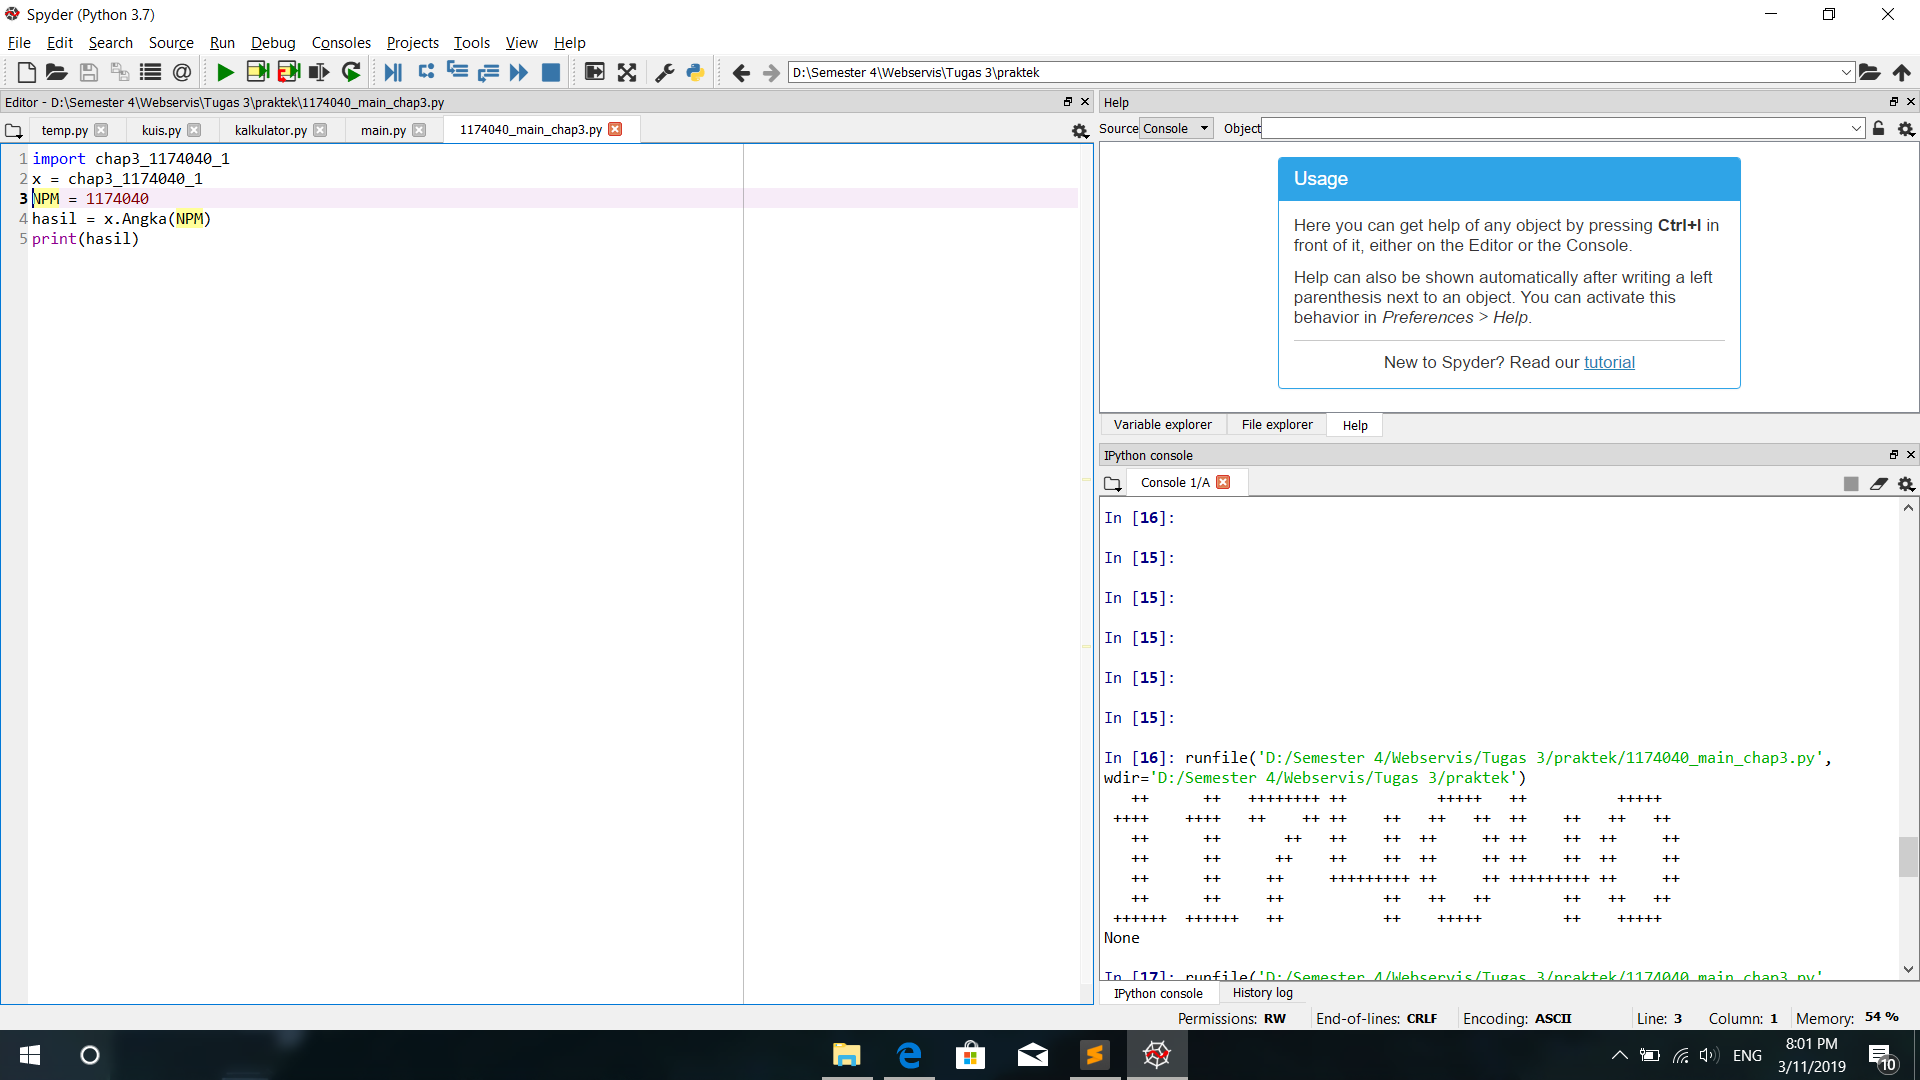
\includegraphics[width=0.5\textwidth]{figures/chapter3/1174040_1.png}}
            \caption{No. 1}
            \label{1174040_no1}
            \end{figure}

            \item \lstinputlisting{src/chapter3/chap3_1174040_2.py}
            \begin{figure}[ht]
            \centerline{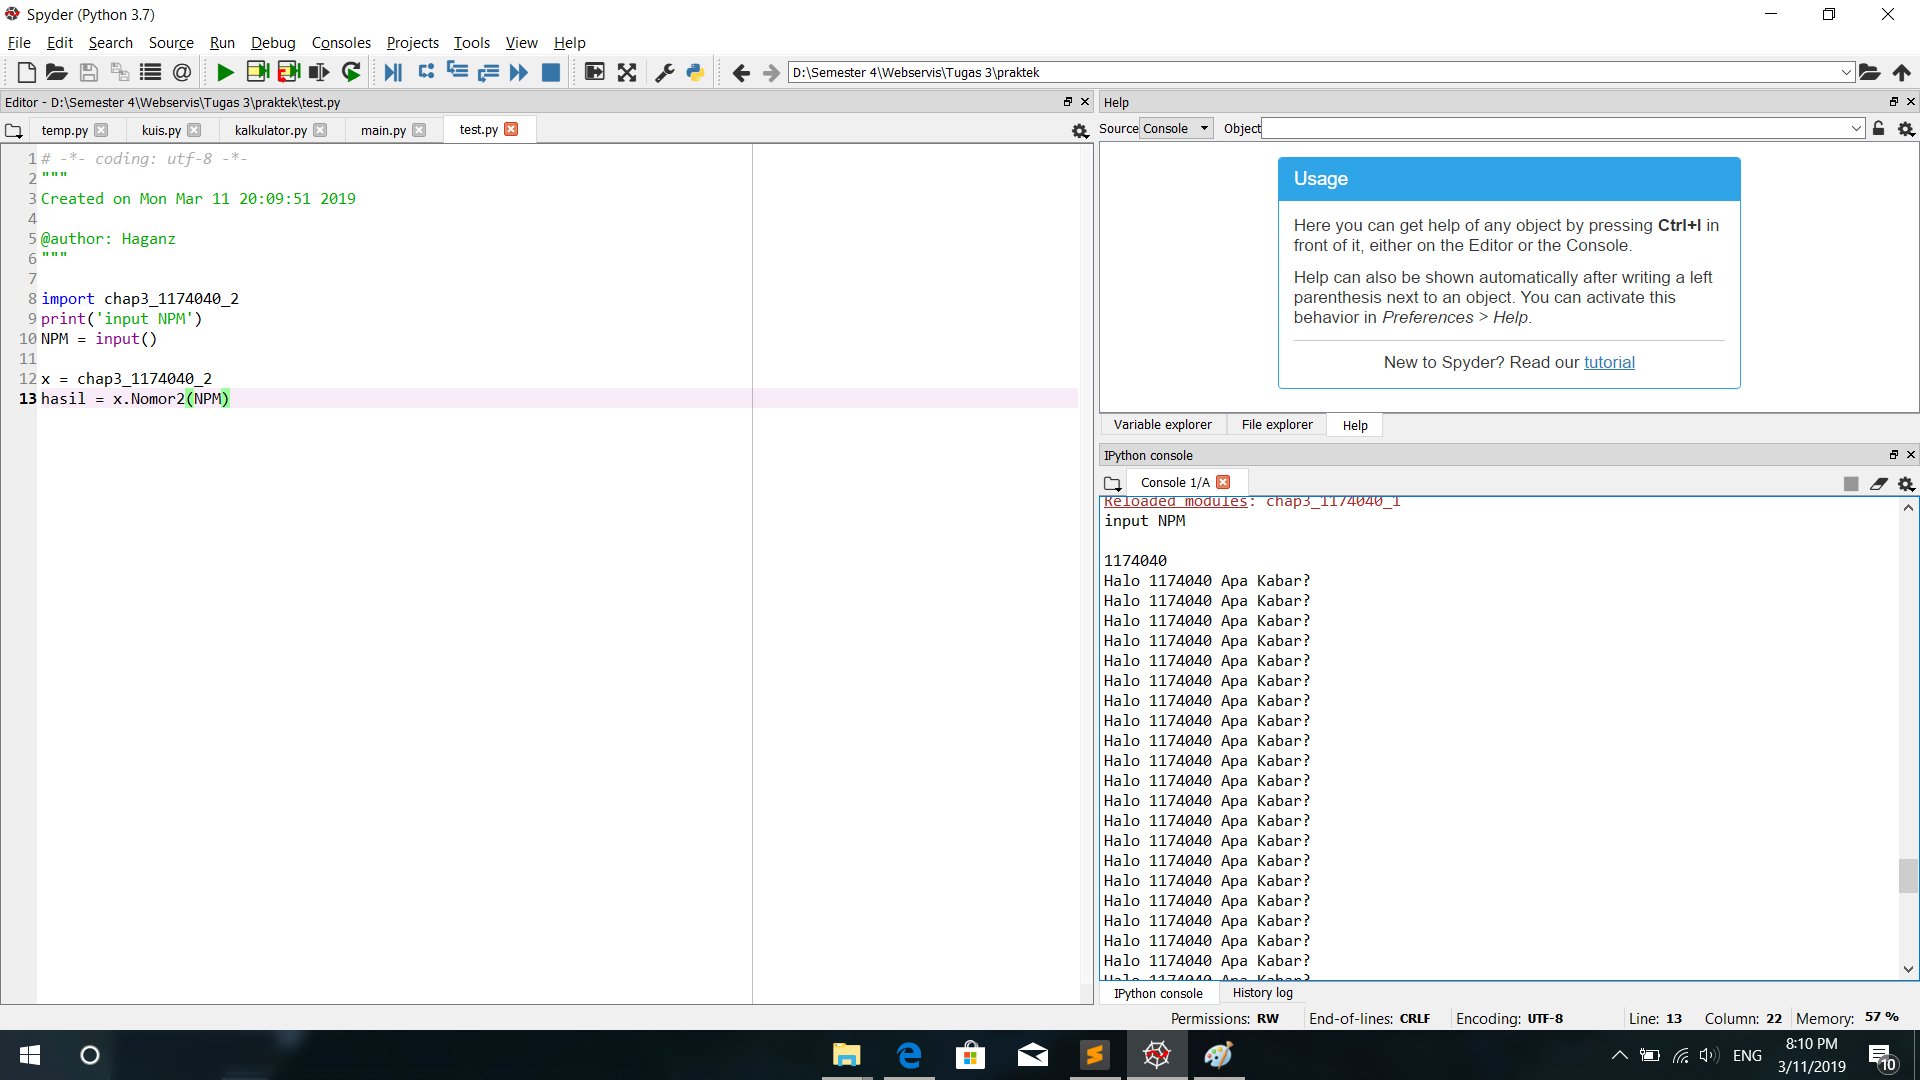
\includegraphics[width=0.5\textwidth]{figures/chapter3/1174040_2.png}}
            \caption{No. 2}
            \label{1174040_no2}
            \end{figure}

            \item \lstinputlisting{src/chapter3/chap3_1174040_3.py}
            \begin{figure}[ht]
            \centerline{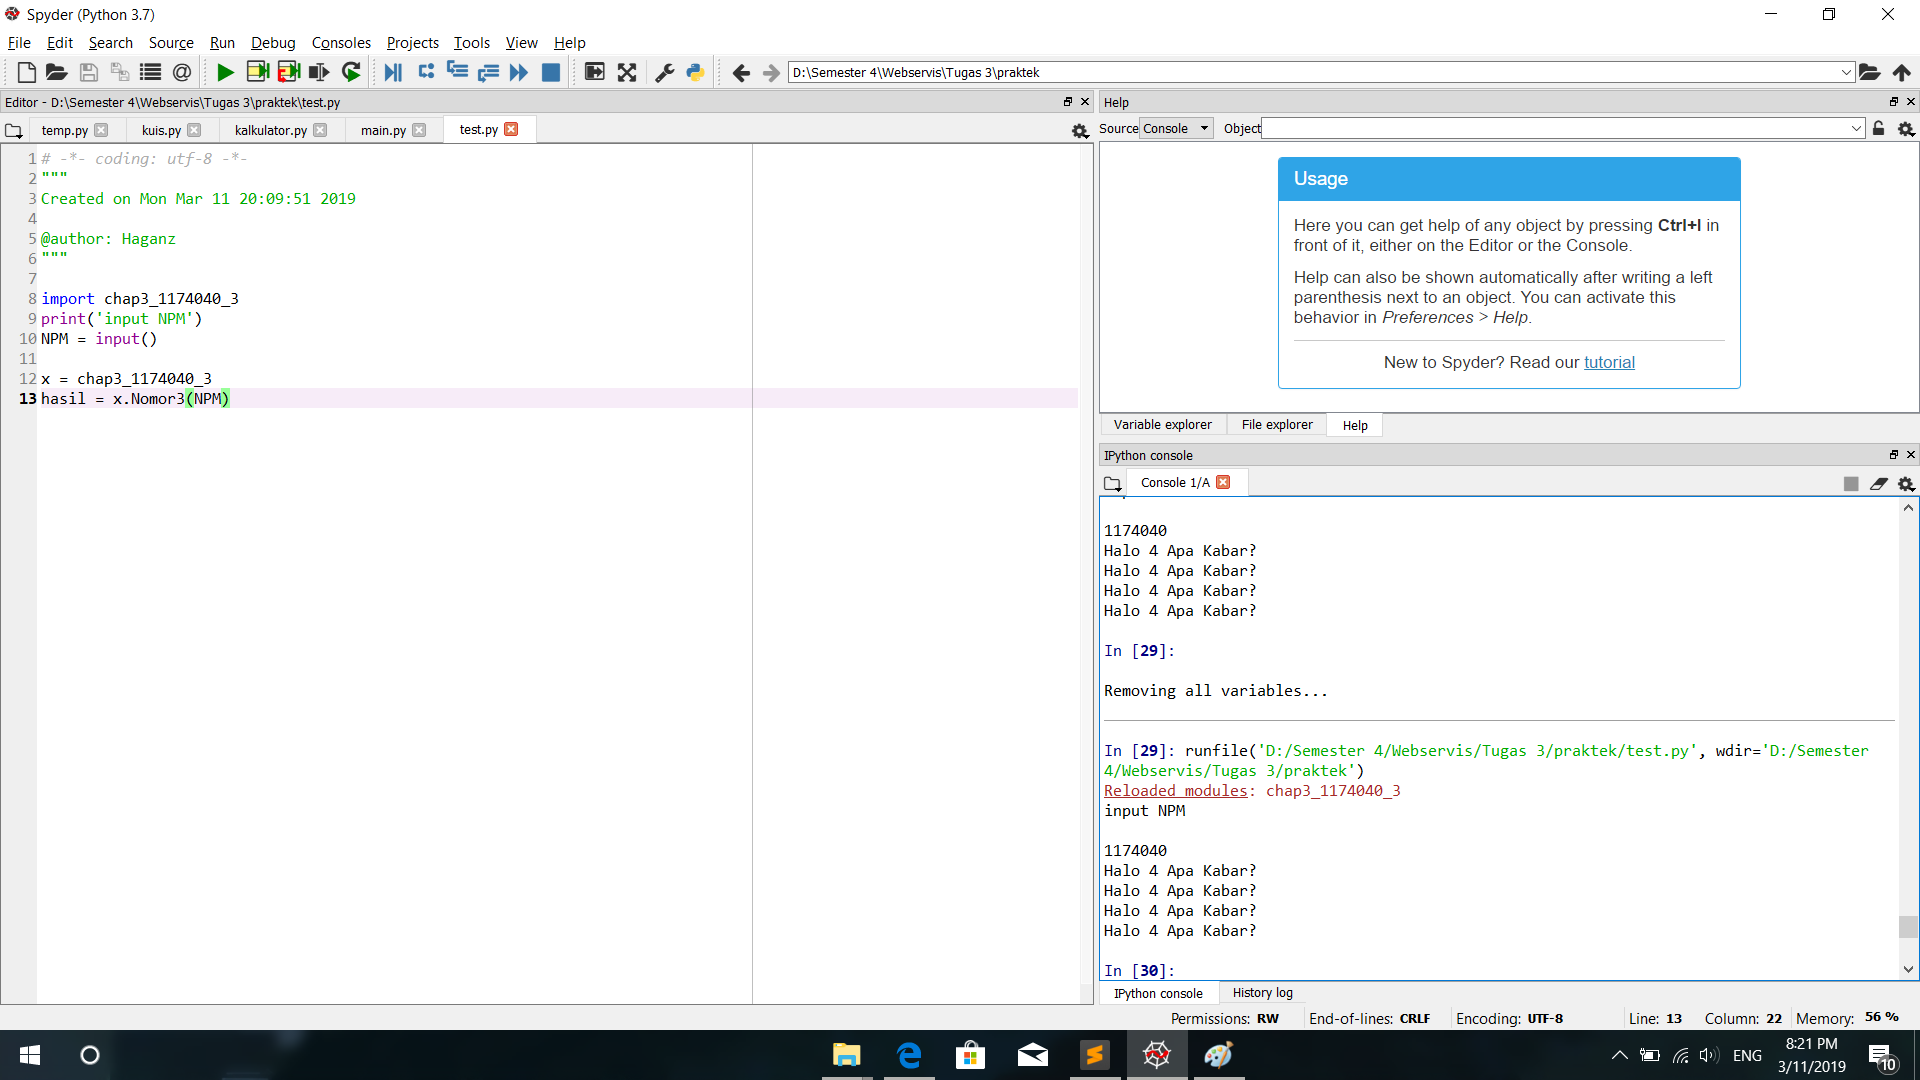
\includegraphics[width=0.5\textwidth]{figures/chapter3/1174040_3.png}}
            \caption{No. 3}
            \label{1174040_no3}
            \end{figure}

            \item \lstinputlisting{src/chapter3/chap3_1174040_4.py}
            \begin{figure}[ht]
            \centerline{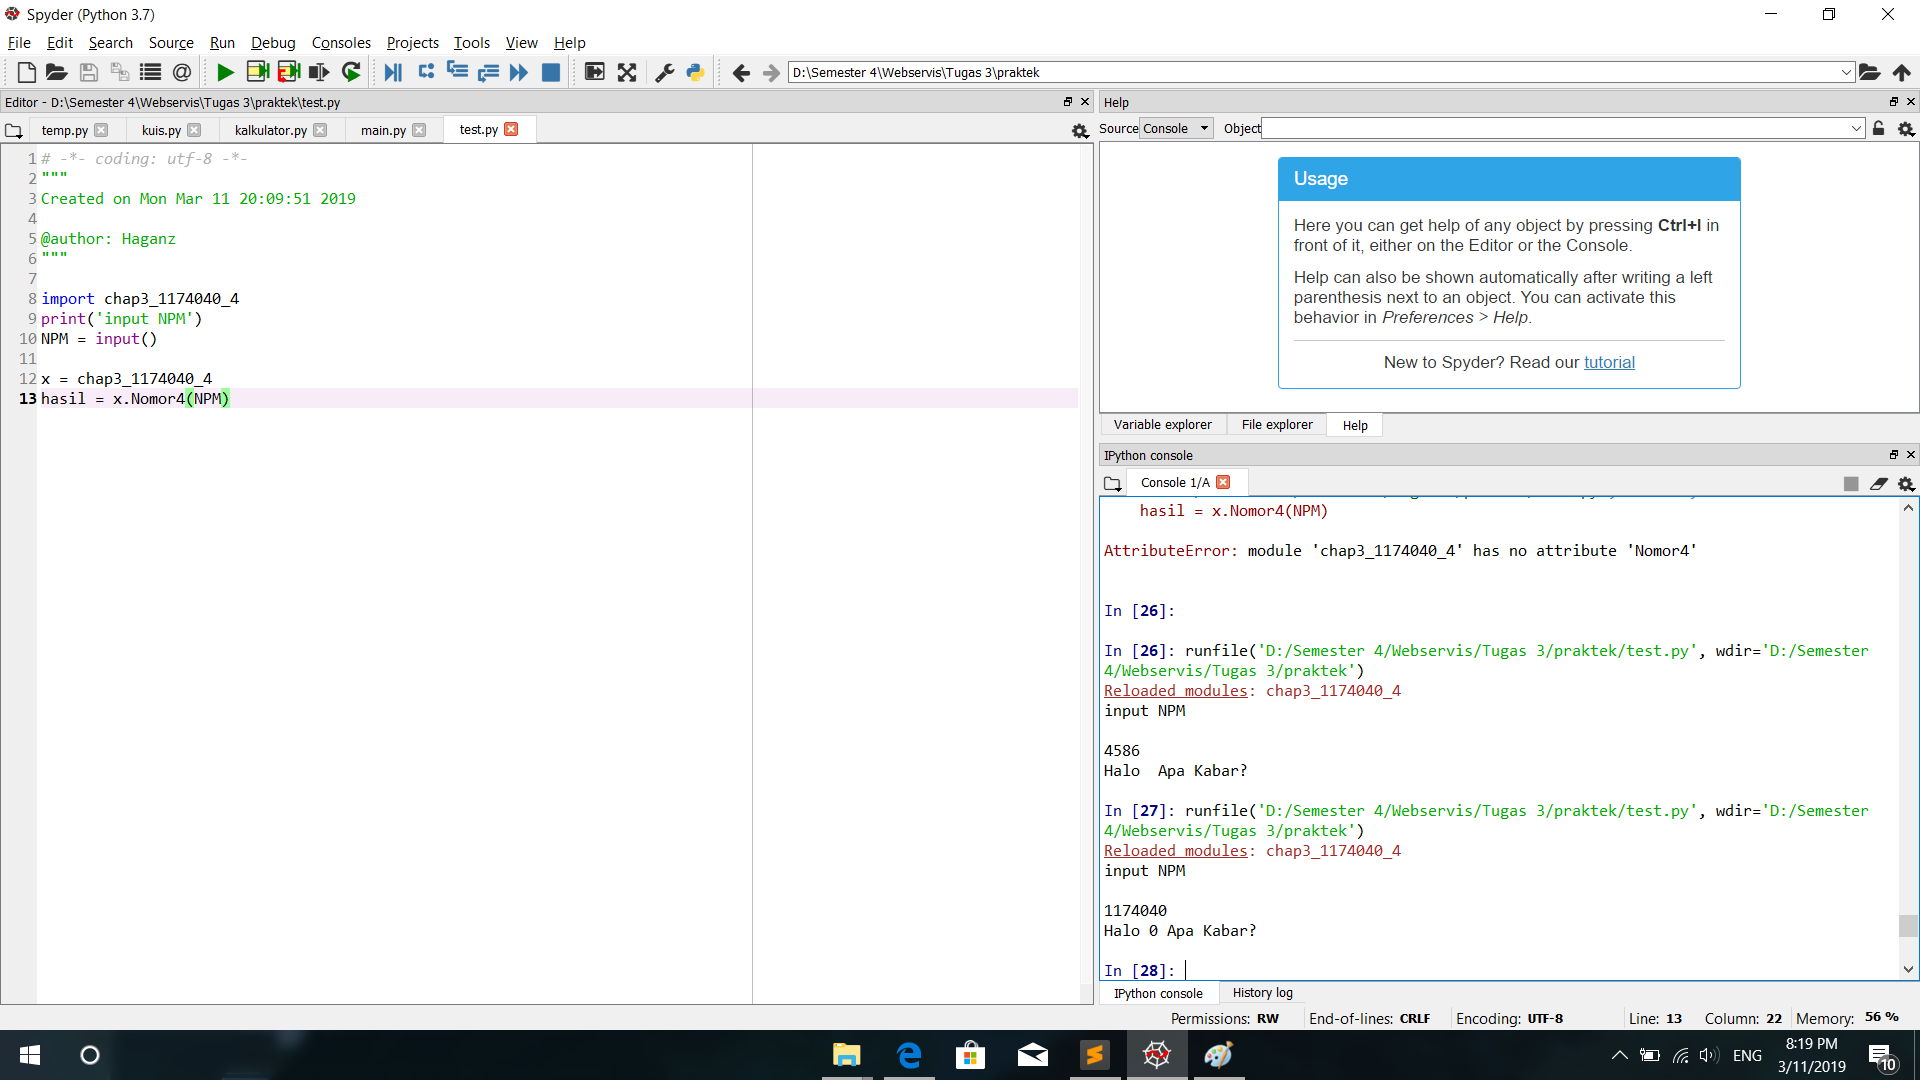
\includegraphics[width=0.5\textwidth]{figures/chapter3/1174040_4.png}}
            \caption{No. 4}
            \label{1174040_no4}
            \end{figure}

            \item \lstinputlisting{src/chapter3/chap3_1174040_5.py}
            \begin{figure}[ht]
            \centerline{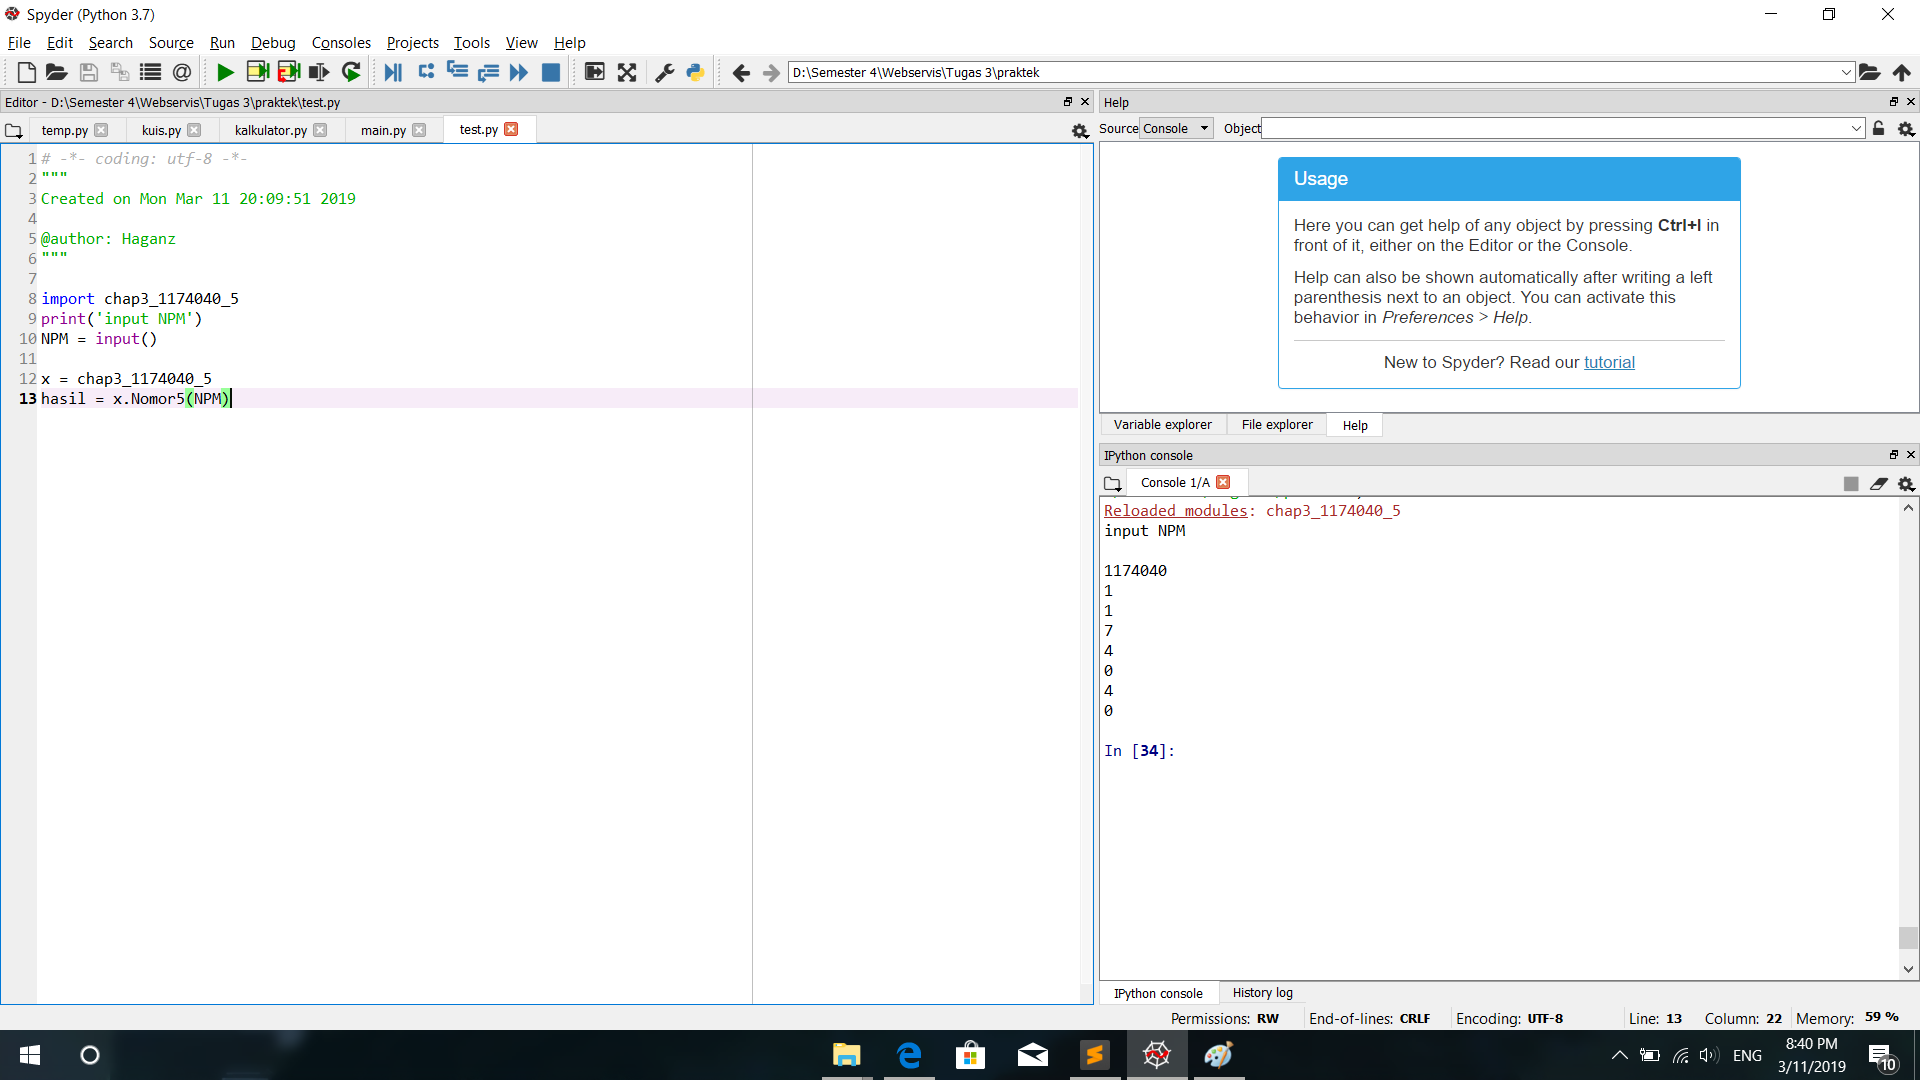
\includegraphics[width=0.5\textwidth]{figures/chapter3/1174040_5.png}}
            \caption{No. 5}
            \label{1174040_no5}
            \end{figure}

            \item \lstinputlisting{src/chapter3/chap3_1174040_6.py}
            \begin{figure}[ht]
            \centerline{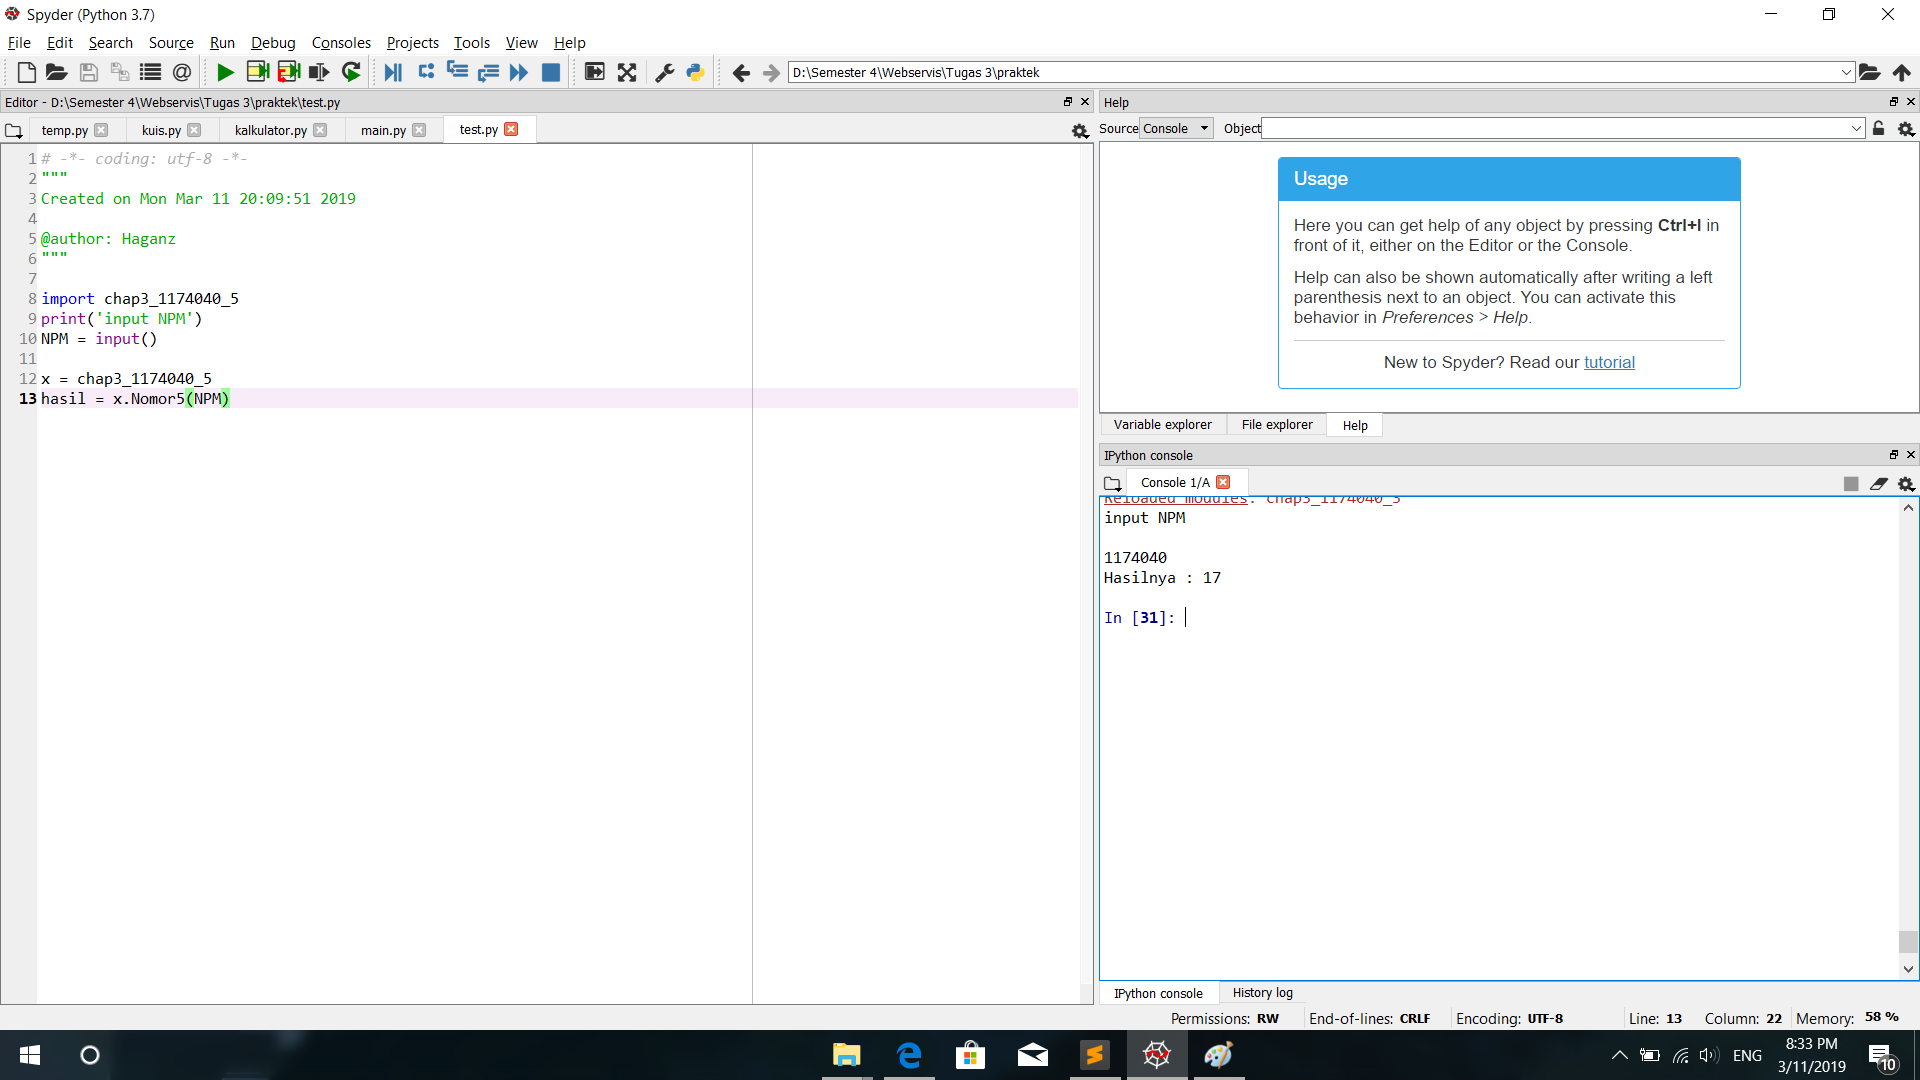
\includegraphics[width=0.5\textwidth]{figures/chapter3/1174040_6.png}}
            \caption{No. 6}
            \label{1174040_no6}
            \end{figure}

            \item \lstinputlisting{src/chapter3/chap3_1174040_7.py}
            \begin{figure}[ht]
            \centerline{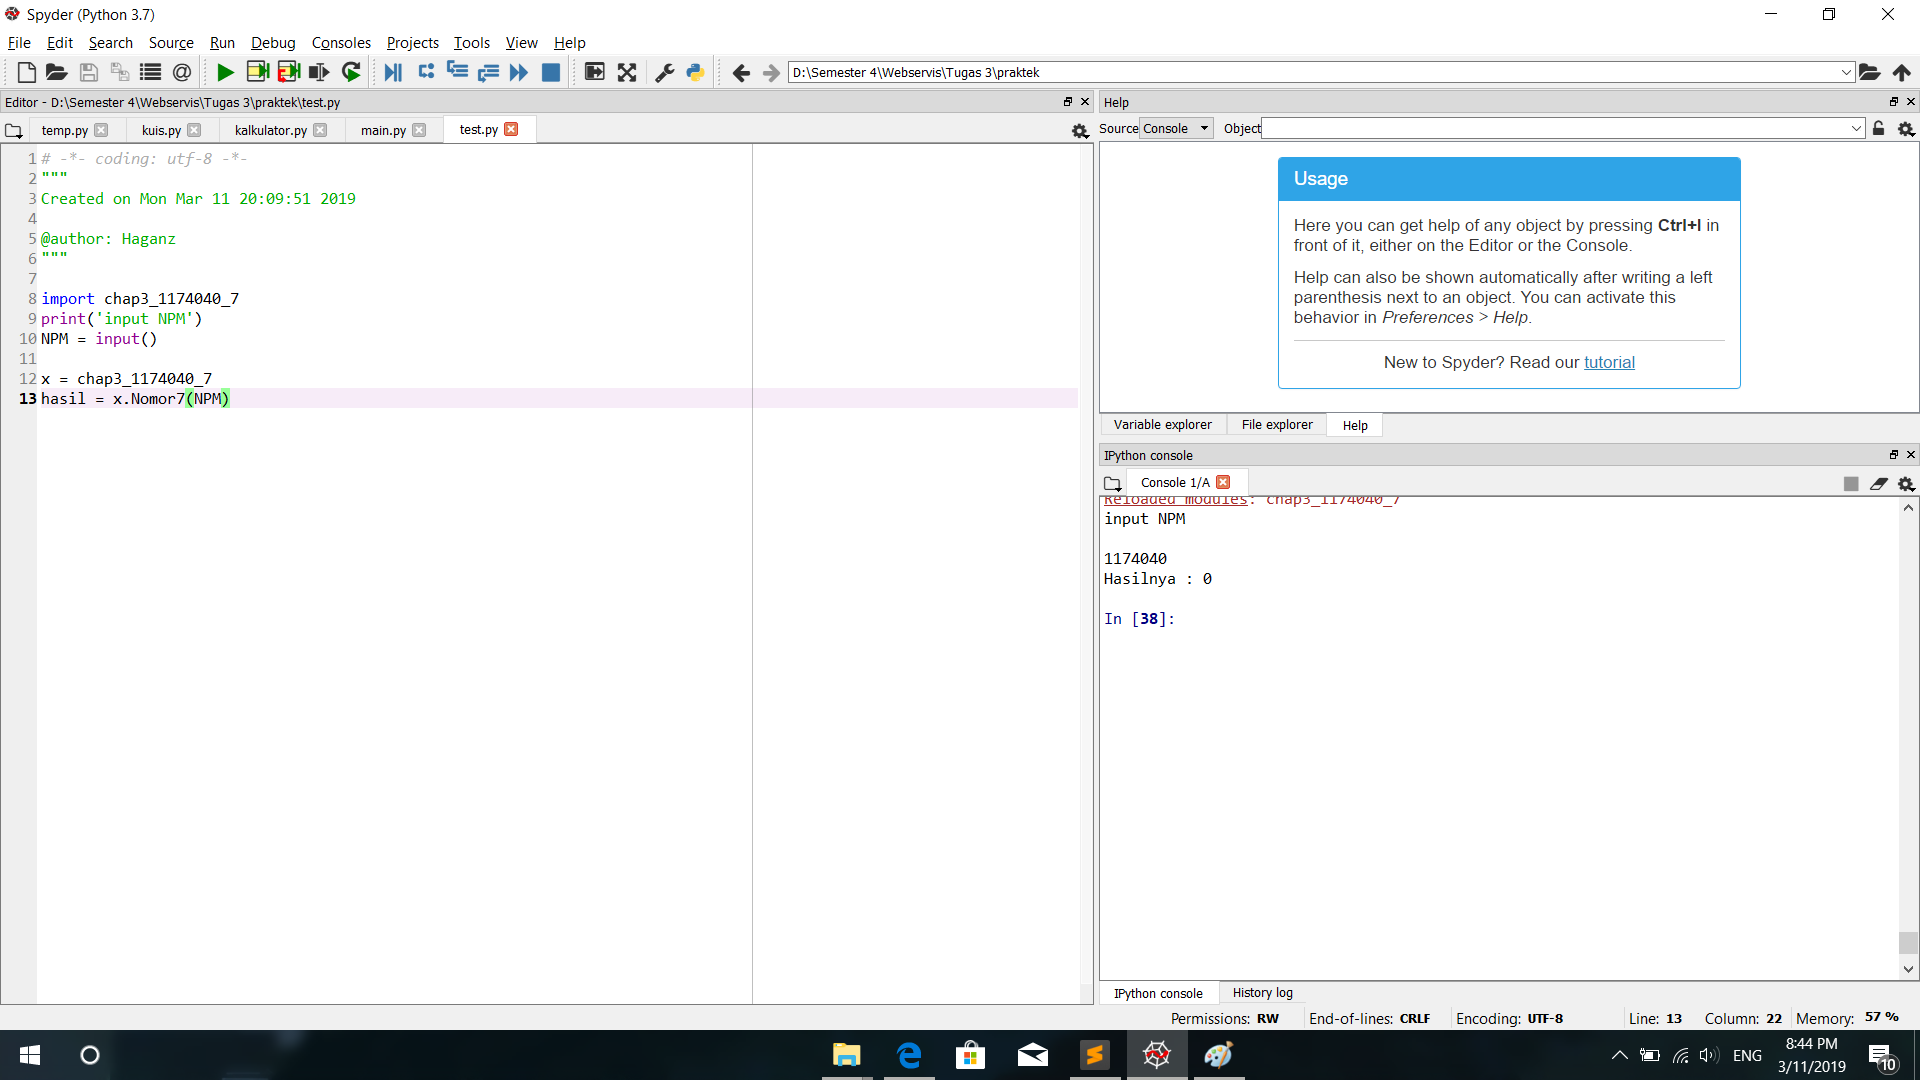
\includegraphics[width=0.5\textwidth]{figures/chapter3/1174040_7.png}}
            \caption{No. 7}
            \label{1174040_no7}
            \end{figure}

            \item \lstinputlisting{src/chapter3/chap3_1174040_8.py}
\begin{figure}[ht]

            \centerline{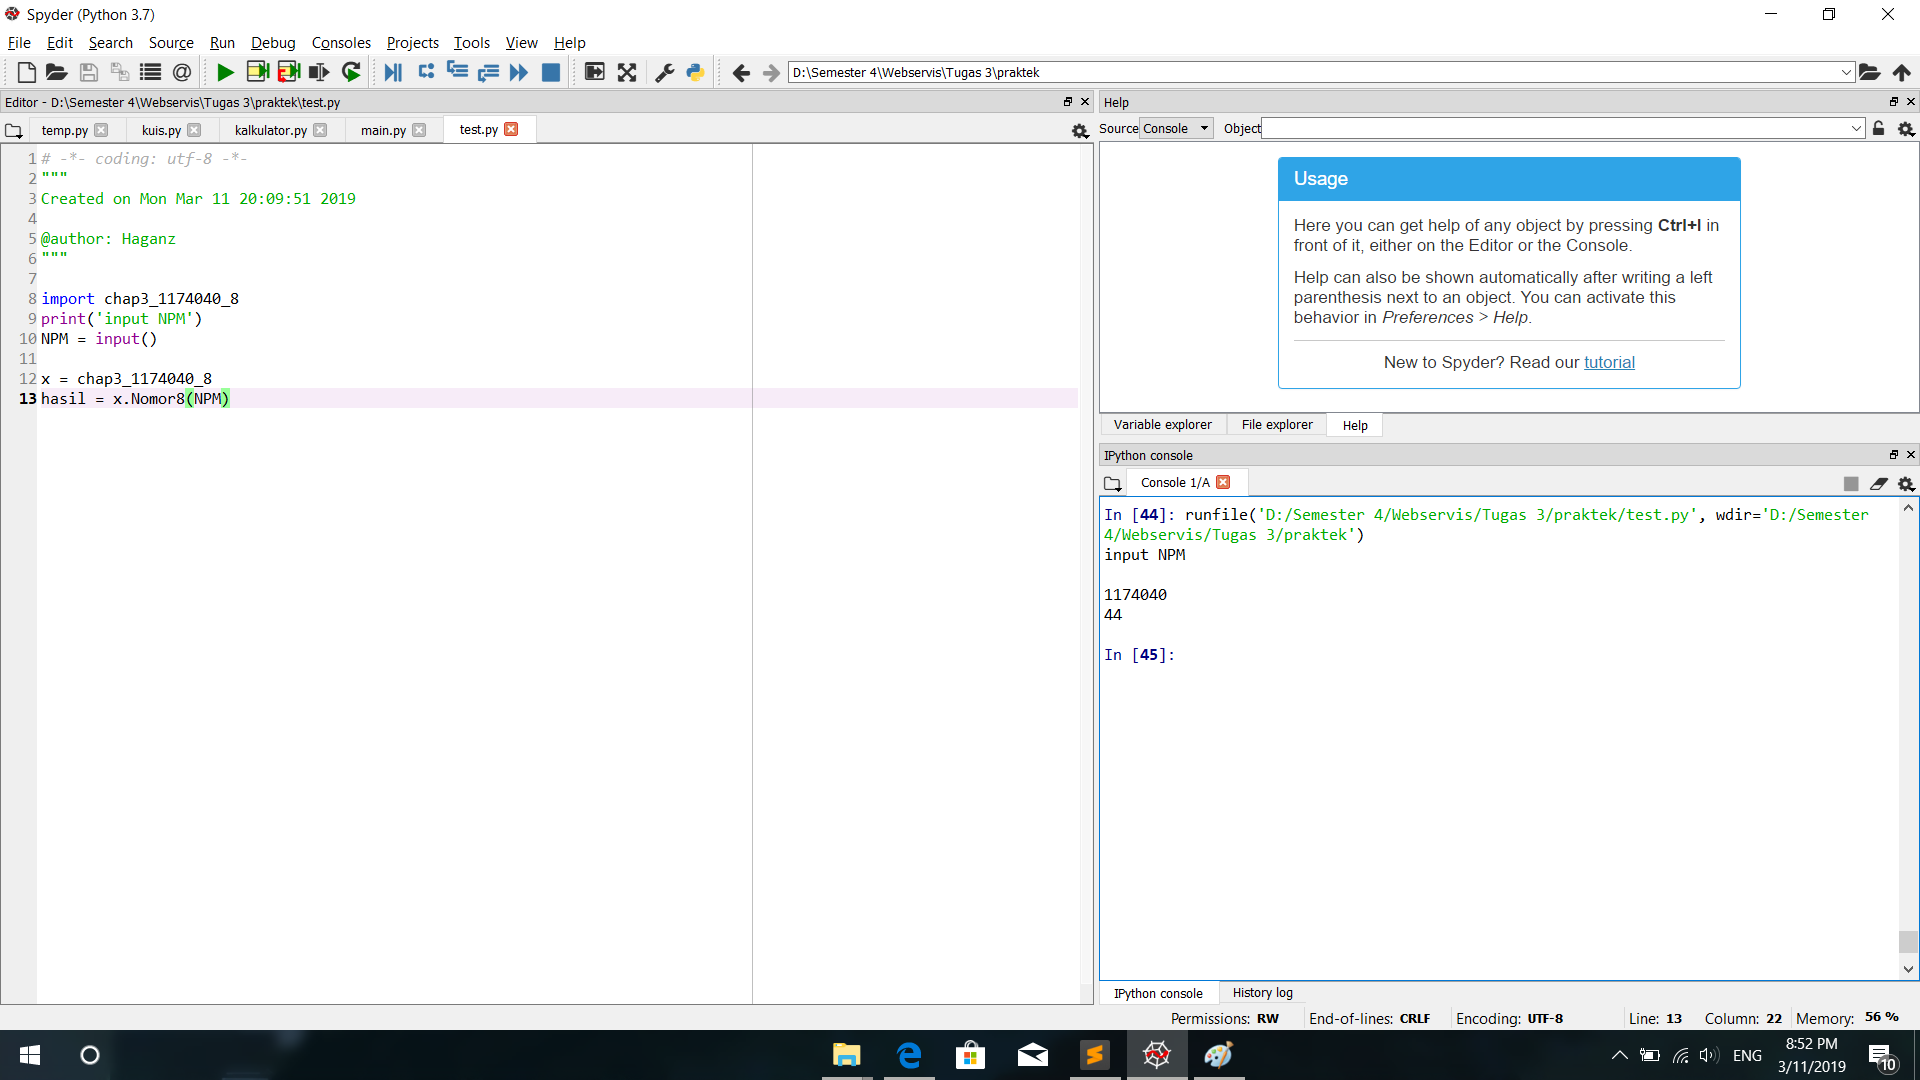
\includegraphics[width=0.5\textwidth]{figures/chapter3/1174040_8.png}}

            \caption{Gambar 8}

            \label{1174040_8}

            \end{figure}

            \item \lstinputlisting{src/chapter3/chap3_1174040_9.py}

\begin{figure}[ht]
            \centerline{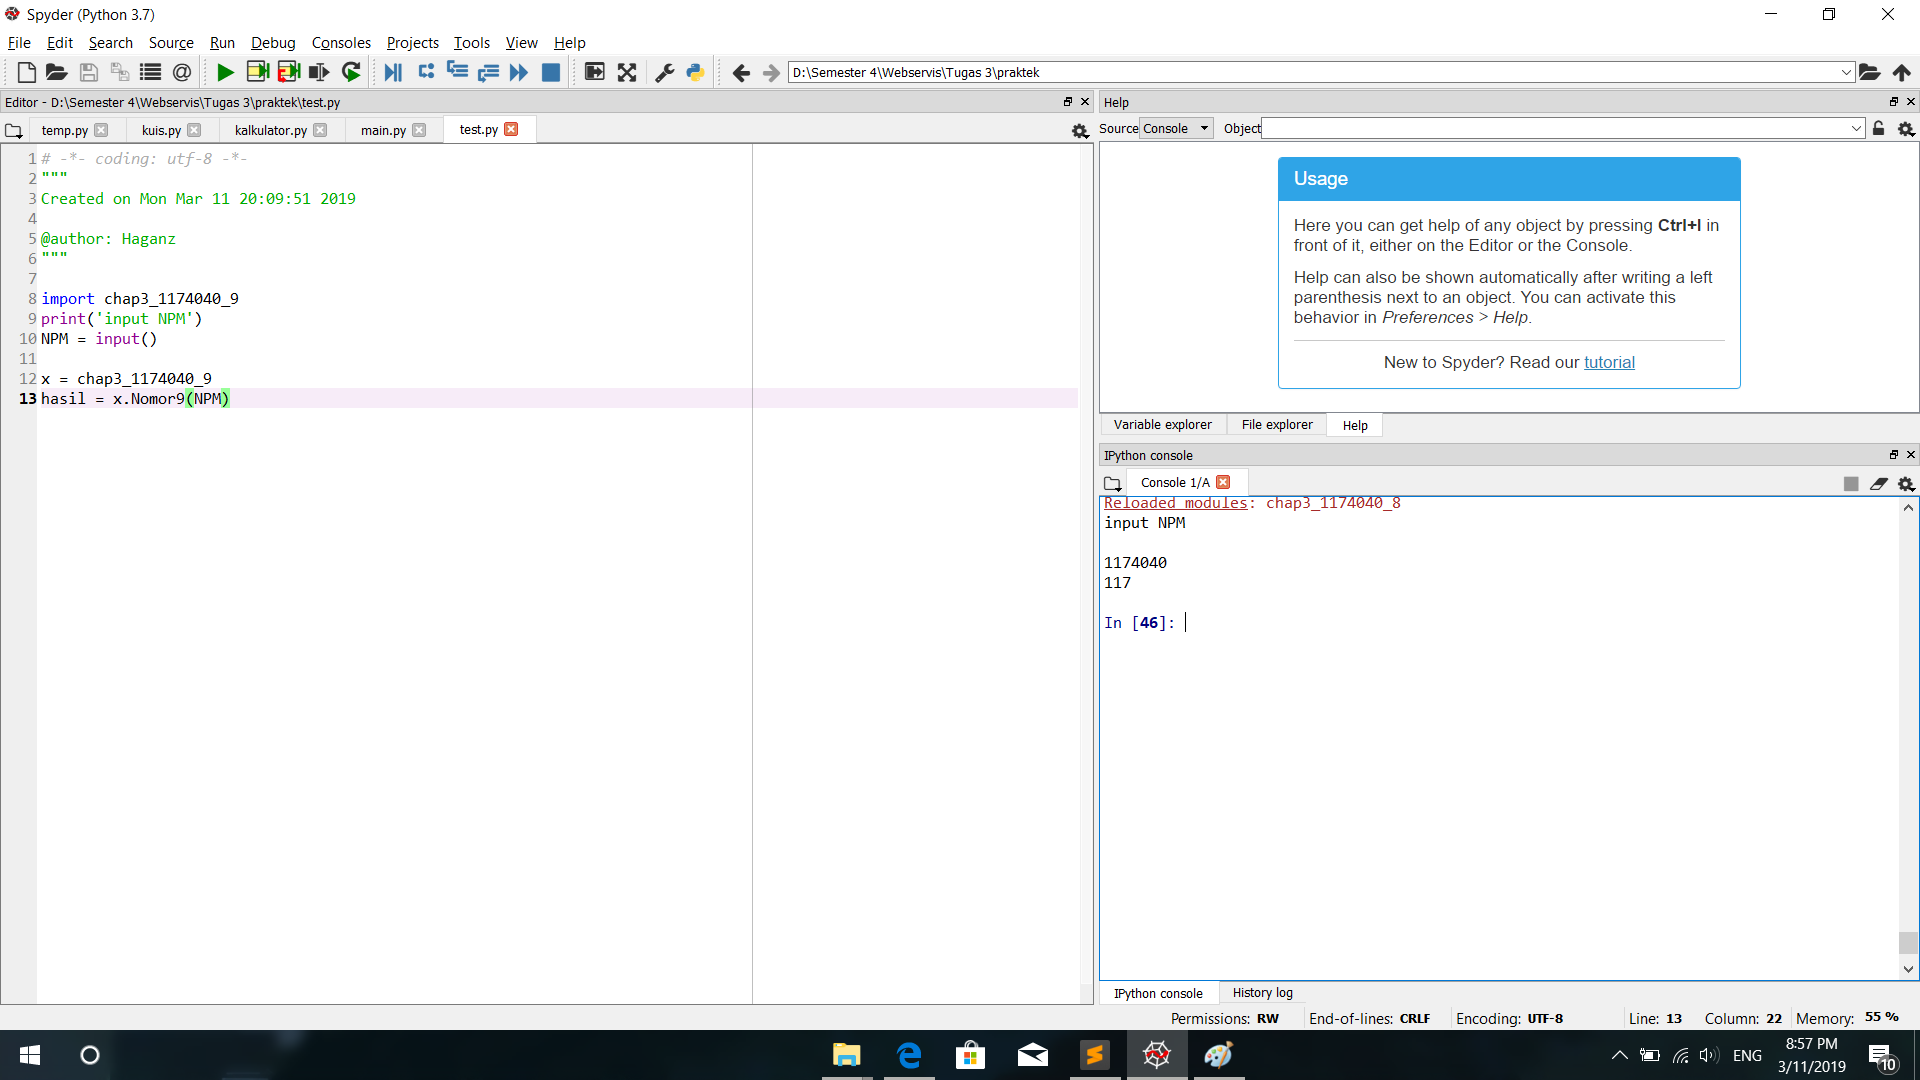
\includegraphics[width=0.5\textwidth]{figures/chapter3/1174040_9.png}}
            \caption{No. 9}
            \label{1174040_no9}
            \end{figure}

            \item \lstinputlisting{src/chapter3/chap3_1174040_10.py}

            \begin{figure}[ht]

            \centerline{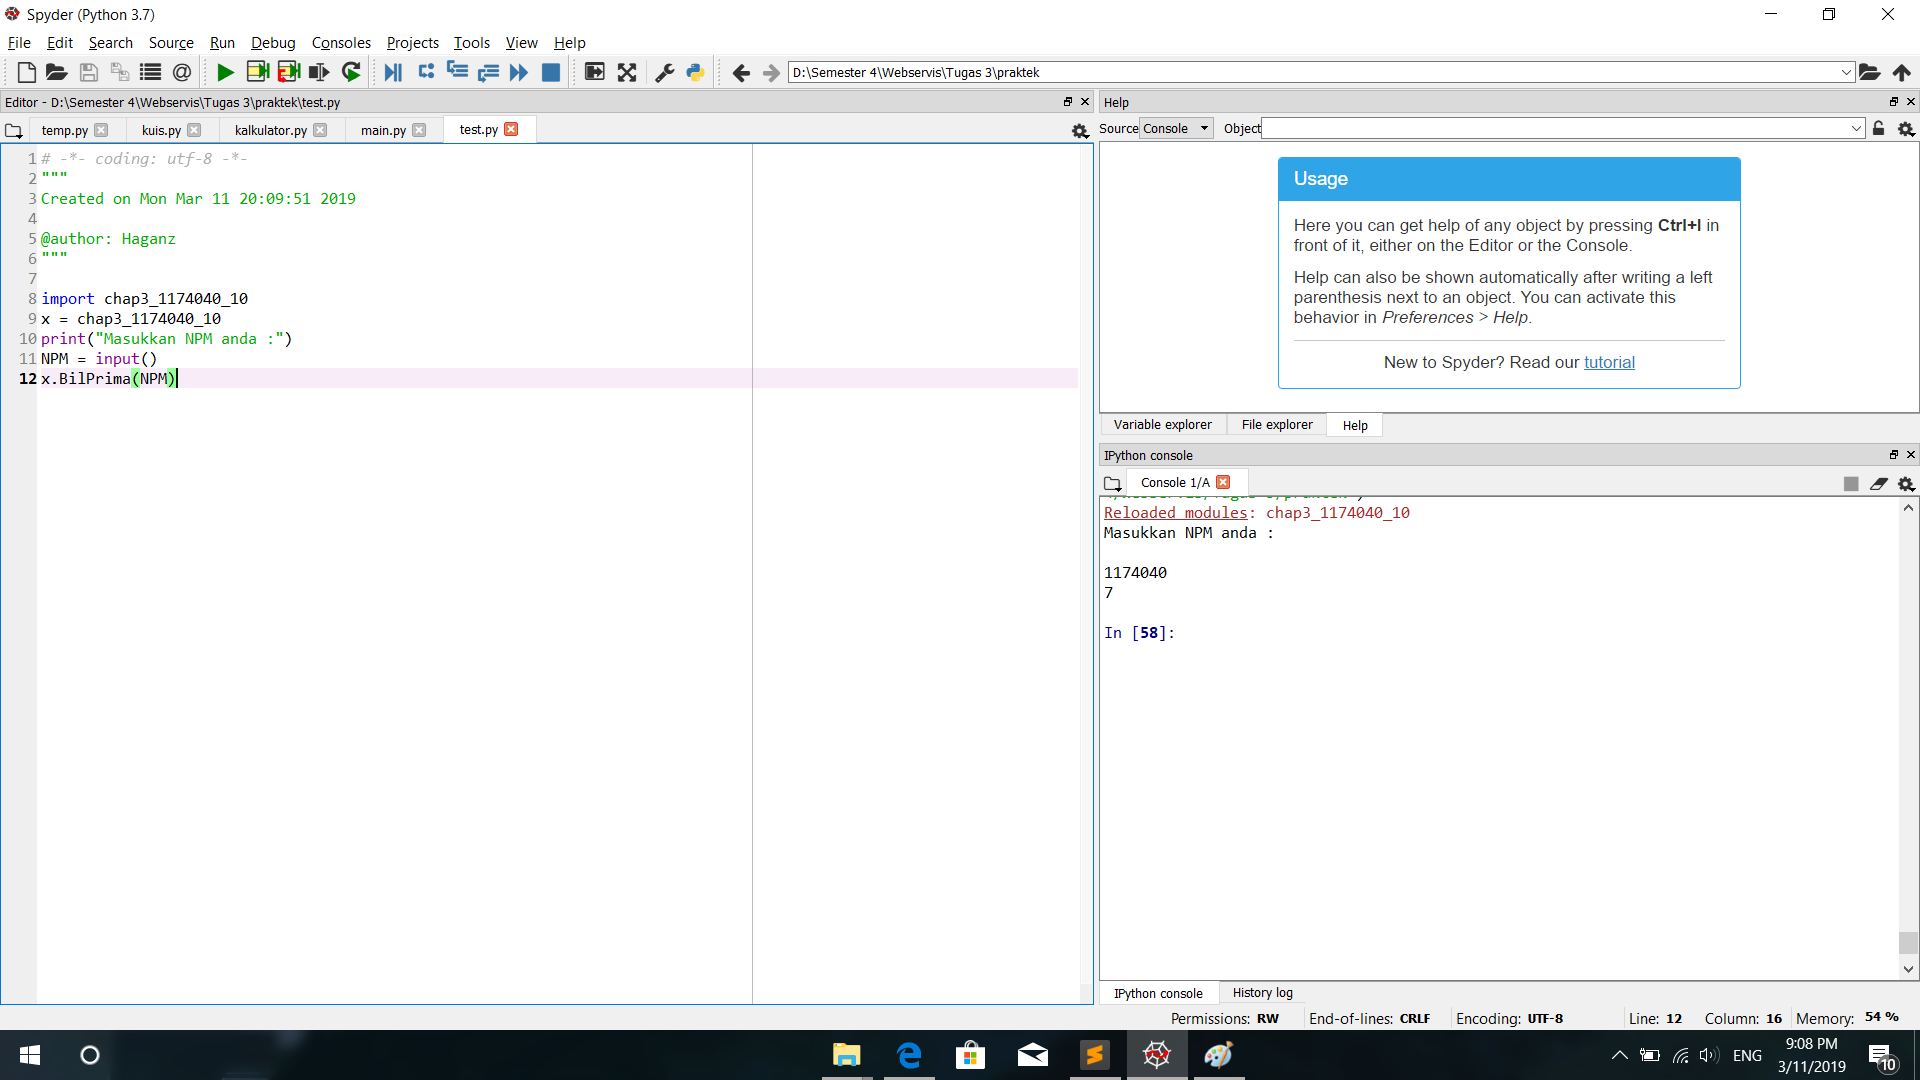
\includegraphics[width=0.5\textwidth]{figures/chapter3/1174040_10.png}}
            \caption{No. 10}
            \label{1174040_no10}
            \end{figure}

            \item Membuat library 3lib.py dan memanggilnya di main.py
            \lstinputlisting[firstline=2, lastline=7]{src/chapter3/chap3_1174040_main.py}
            \begin{figure}[ht]

            \centerline{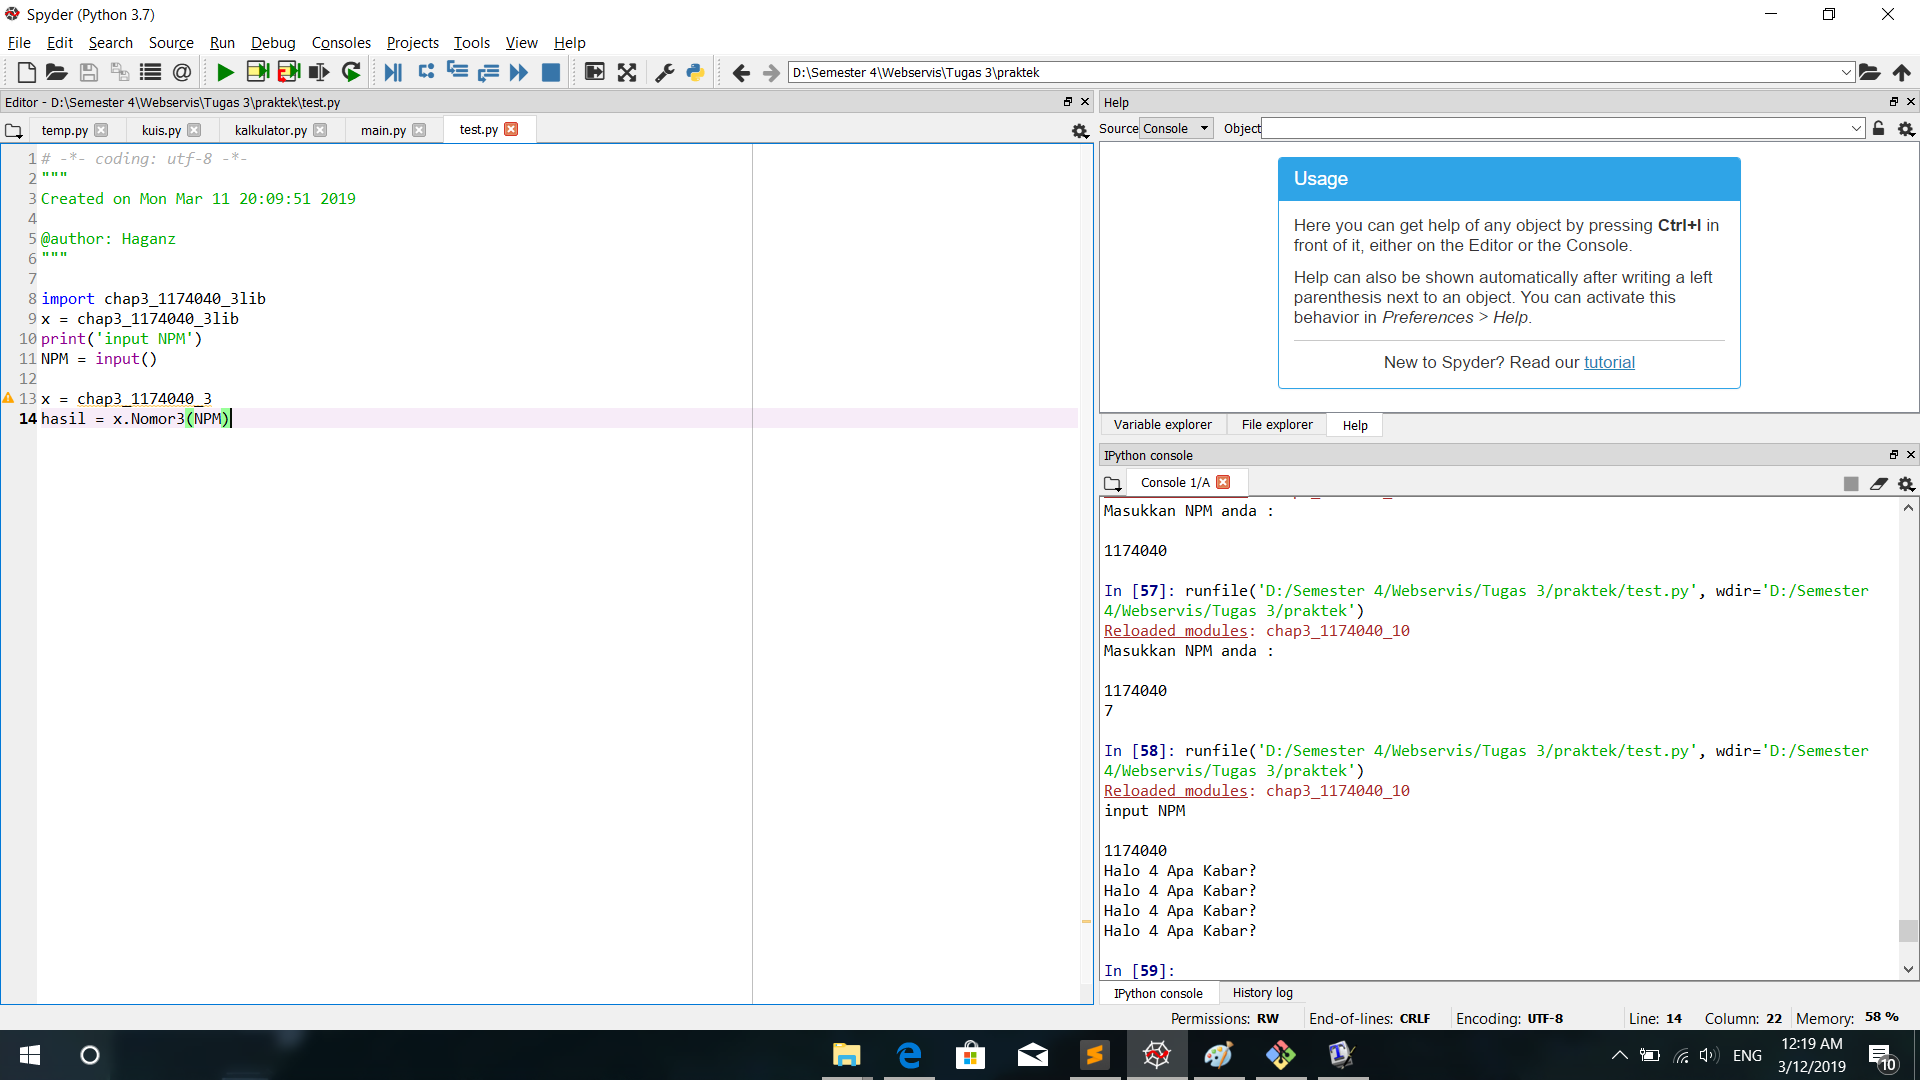
\includegraphics[width=0.5\textwidth]{figures/chapter3/1174040_11.png}}
            \caption{No. 11}
            \label{1174040_no11}
            \end{figure}

            \item Membuat library kelas dengan nama kelas3lib.py yang merupakan modifikasi dari fungsi - fungsi diatas dan berikan contoh pemanggilannya di main.py
            \lstinputlisting[firstline=10, lastline=14]{src/chapter3/chap3_1174040_main.py}
            \begin{figure}[ht]

            \centerline{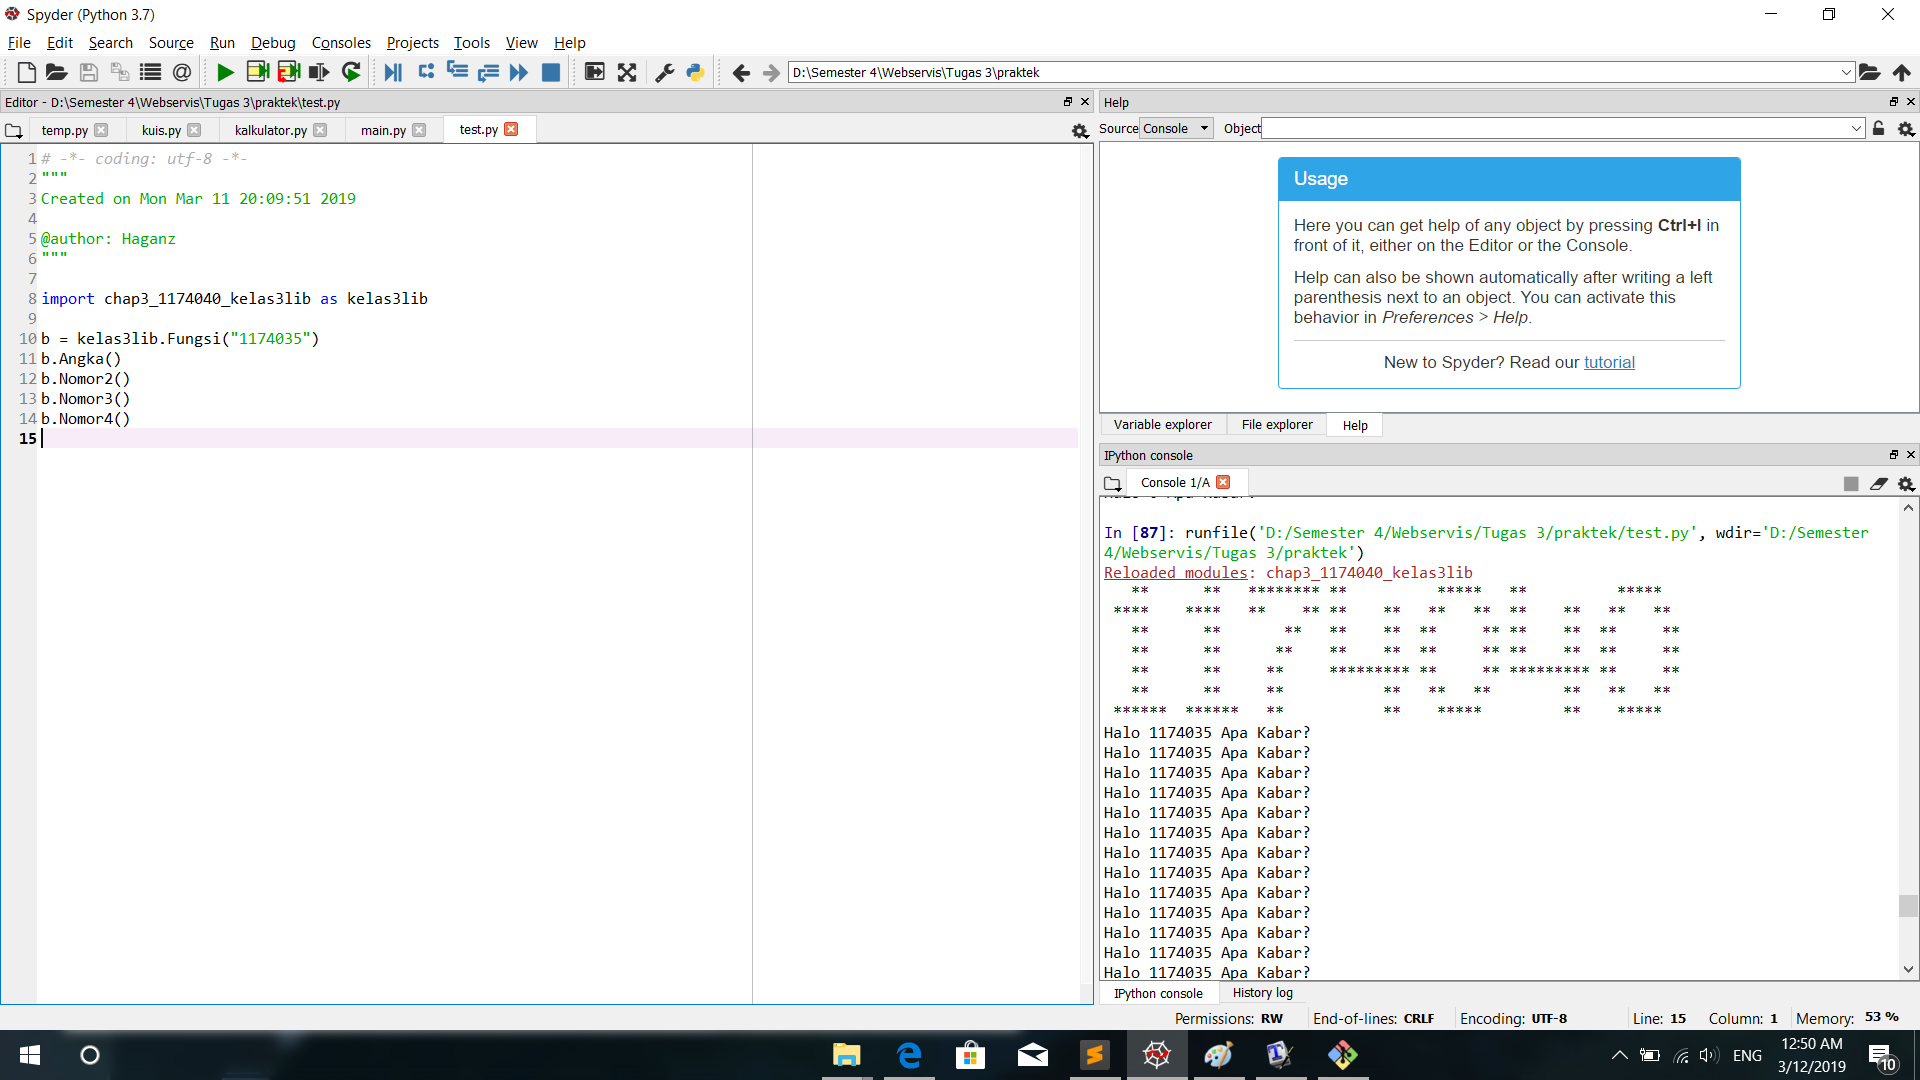
\includegraphics[width=0.5\textwidth]{figures/chapter3/1174040_12.png}}
            \caption{No. 12}
            \label{1174040_no12}
            \end{figure}

        \end{enumerate}
    \subsection{Keterampilan Penanganan Error}
        \begin{enumerate}
            \item Type error karena hasil dari input() adalah string jadi jika masuk kedalam perhitungan dan perbandingan, harus terlebih dahulu diubah menjadi tipe data integer.
            Contoh try dan catch adalah :

            \lstinputlisting{src/chapter3/chap3_1174040_3err.py}
        \end{enumerate}
    \subsection{Cek Plagiarisme}
    \begin{figure}[ht]

            \centerline{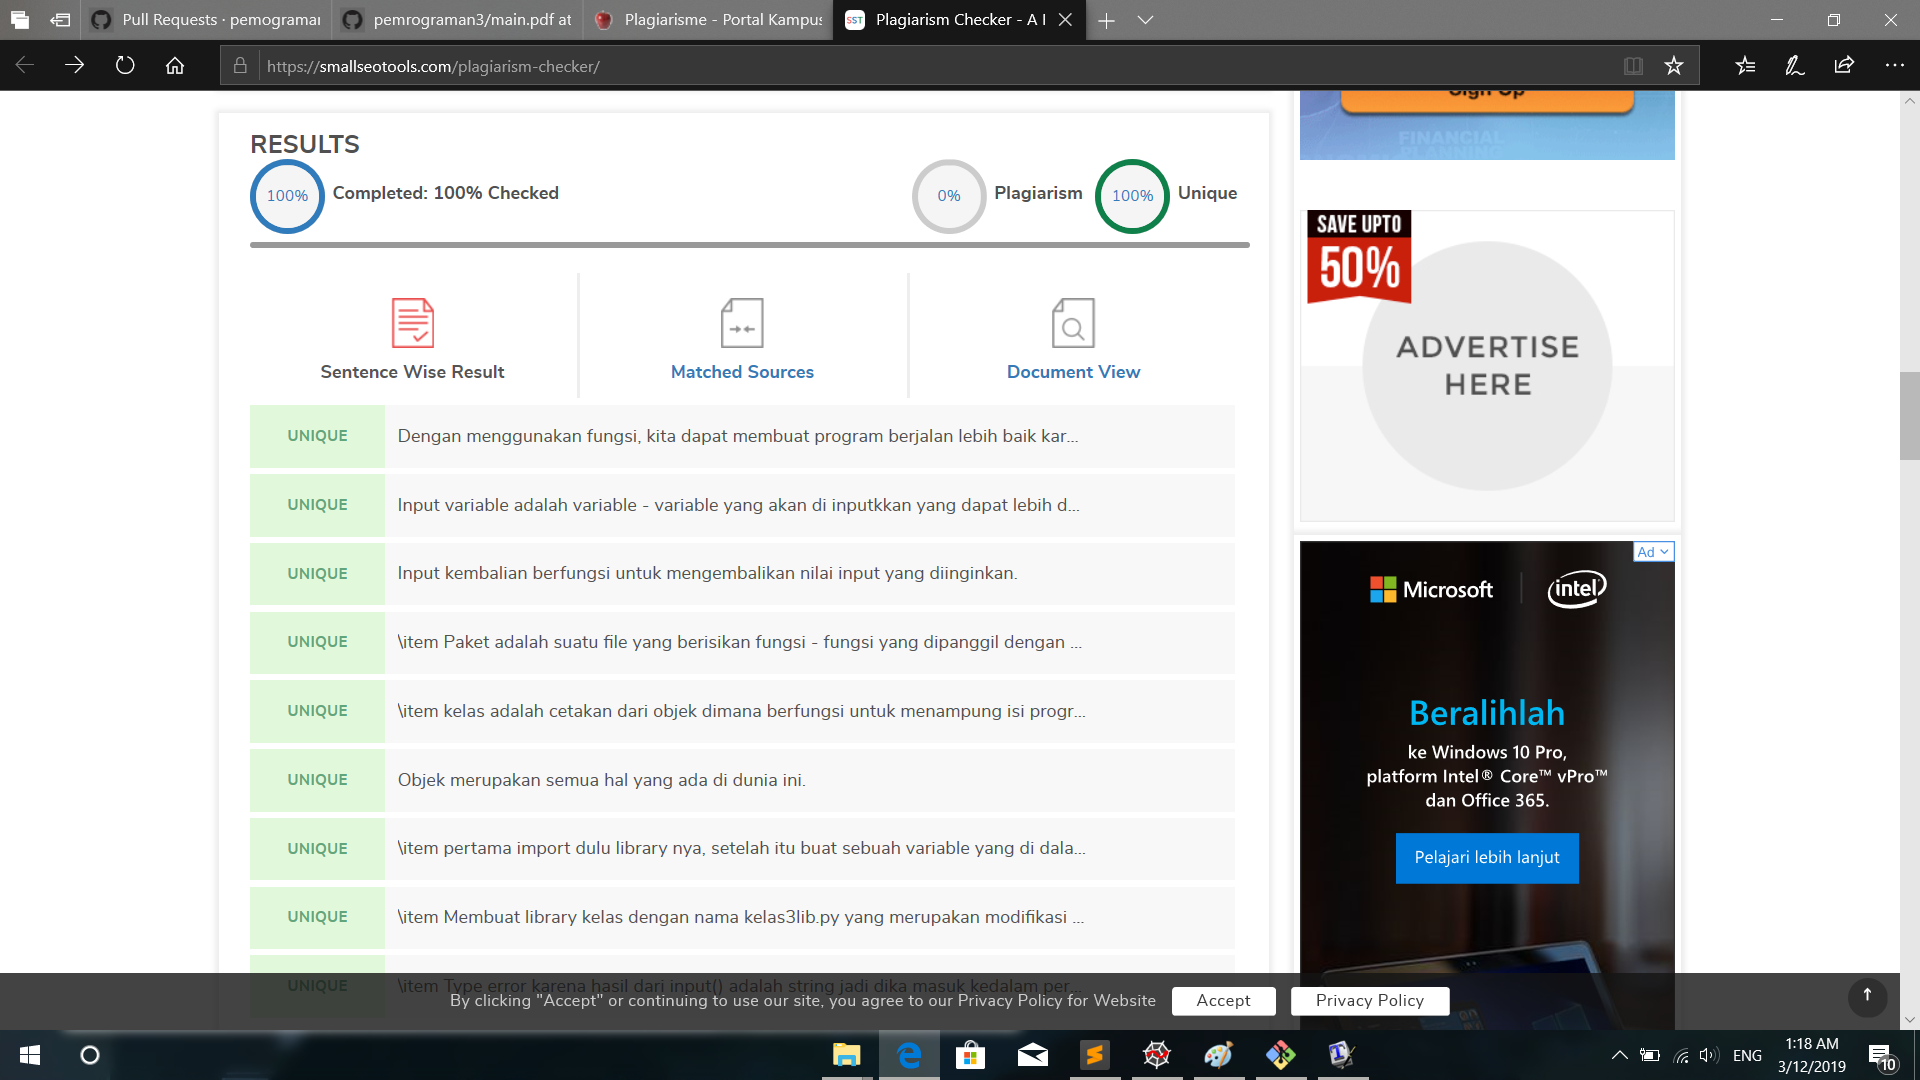
\includegraphics[width=0.5\textwidth]{figures/chapter3/1174040_plagiat.png}}
            \caption{Cek Plagiarisme}
            \label{1174040_cekplagiat}
            \end{figure}

\section{IrvanRizkiansyah/1174043}
	\subsection{Pemahaman Teori}
		\begin{enumerate}
			\item	\begin{itemize}
						\item Fungsi adalah bagian dari program yang berupa blok kode yang diberikan nama dan nama tersebut berguna untuk memanggil fungsi tersebut.
					
						\item Inputan fungsi adalah sebuah fungsi yang telah di sediakan pada library python, yang berguna untuk menerima inputan dari user.
					
						\item Kembalian fungsi adalah sebuah nilai balikan yang diberikan oleh sebuah fungsi yang dibuat.
					\end{itemize}
					
					Contoh Program : 
					\lstinputlisting[language=Python, firstline=2, lastline=8]{src/chapter3/teori_1174043_chap3.py}
					
			\item paket adalah sebuah cara yang dilakukan untuk memanggil file script python, yang nantinya akan digunakan fungsi fungsi yang terdapat pada file script yang dipanggil tersebut. cara pemanggilan paket dengan cara :
				\begin{verbatim}
				import scriptFilePython
				\end{verbatim}
			
			Contoh Program :
			\lstinputlisting[language=Python, firstline=11, lastline=11]{src/chapter3/teori_1174043_chap3.py}
			
			\item	\begin{itemize}
						\item Kelas merupakan sebuah cetakan atau Blueprint yang berguna untuk mencetak objek.
						
						\item Objek merupakan sebuah objek yang dari proses hasil dari cetakan atau blueprint.
						
						\item Atribut merupakan penggambaran data yang bisa memberikan sebuah informasi kelas atau objek dimana atribut tersebut berada.
						
						\item Method merupakan fungsi atau prosedur yang bergabung dengan sebuah objek dan juga atribut.
					\end{itemize}
					
					Contoh Program :
					\lstinputlisting[language=Python, firstline=14, lastline=17]{src/chapter3/teori_1174043_chap3.py}
					
			\item cara pemanggilan library kelas dari instansiasi, adalah dengan cara mengubah library kelas yang dipanggil menjadi sebuah objek.
			
			Contoh Program : 
			\lstinputlisting[language=Python, firstline=22, lastline=24]{src/chapter3/teori_1174043_chap3.py}
			
			\item Jadi pemakaian paket dengan perintah from kalkulator import penambahan berguna untuk menghemat memori pemakaian pada program, karena hanya memanggil fungsi yang diperlukan saja pada library yang terpanggil. cara memanggilnya dengan cara :
				\begin{verbatim}
				from scripFilePython import namaFungsi, namaFungsi2
				\end{verbatim}
				
			Contoh Program :
			\lstinputlisting[language=Python, firstline=27, lastline=27]{src/chapter3/teori_1174043_chap3.py}
			
			\item \lstinputlisting[language=Python, firstline=30, lastline=35]{src/chapter3/teori_1174043_chap3.py}
			
			\item \lstinputlisting[language=Python, firstline=38, lastline=42]{src/chapter3/teori_1174043_chap3.py}
			
		\end{enumerate}
		
	\subsection{Keterampilan Pemrograman}
		\begin{enumerate}
			\item Jawaban soal no 1
				\lstinputlisting{src/chapter3/chap3_1174043_no1.py}
				
				\begin{figure} [ht]
					\centerline{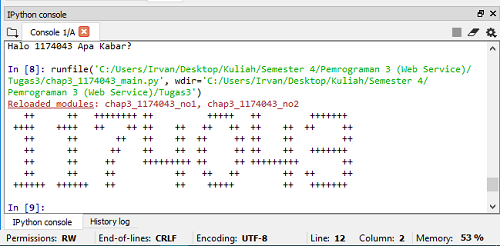
\includegraphics[width=0.6\textwidth]{figures/chapter3/1_1174043.png}}
					\caption{Jawaban No. 1}
					\label{1}
				\end{figure}

				\ref{1_1174043}
				
			\item Jawaban soal no 2
				\lstinputlisting{src/chapter3/chap3_1174043_no2.py}
				
				\begin{figure} [ht]
					\centerline{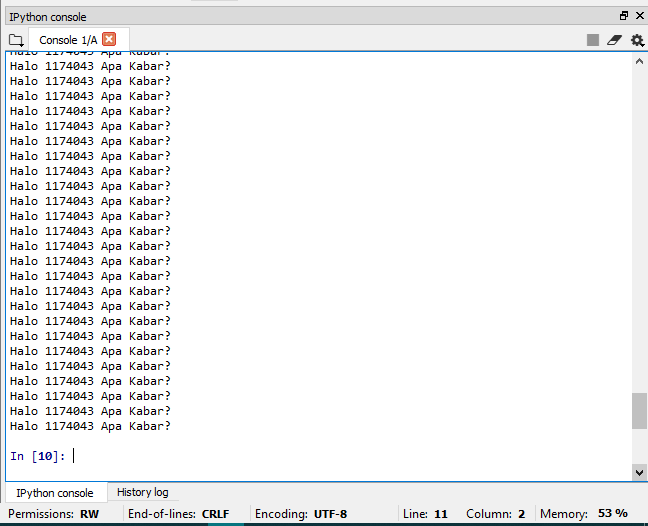
\includegraphics[width=1\textwidth]{figures/chapter3/2_1174043.png}}
					\caption{Jawaban No. 2}
					\label{2}
				\end{figure}

				\ref{2_1174043}
			
			\item Jawaban soal no 3
				\lstinputlisting{src/chapter3/chap3_1174043_no3.py}
				
				\begin{figure} [ht]
					\centerline{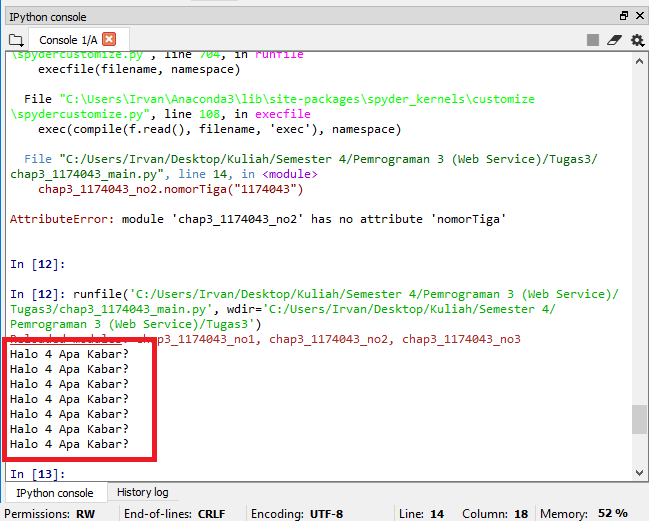
\includegraphics[width=1\textwidth]{figures/chapter3/3_1174043.png}}
					\caption{Jawaban No. 3}
					\label{3}
				\end{figure}

				\ref{3_1174043}
				
			\item Jawaban soal no 4
				\lstinputlisting{src/chapter3/chap3_1174043_no4.py}
				
				\begin{figure} [ht]
					\centerline{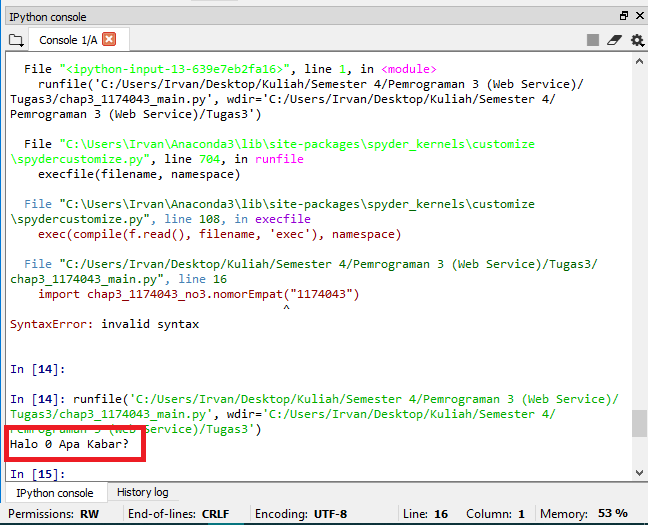
\includegraphics[width=1\textwidth]{figures/chapter3/4_1174043.png}}
					\caption{Jawaban No. 4}
					\label{4}
				\end{figure}

				\ref{4_1174043}
				
			\item Jawaban soal no 5
				\lstinputlisting{src/chapter3/chap3_1174043_no5.py}
				
				\begin{figure} [ht]
					\centerline{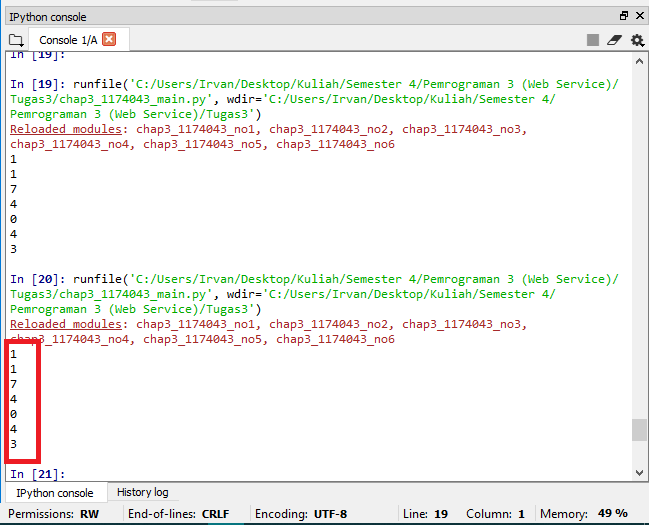
\includegraphics[width=1\textwidth]{figures/chapter3/5_1174043.png}}
					\caption{Jawaban No. 5}
					\label{5}
				\end{figure}

				\ref{5_1174043}
				
			\item Jawaban soal no 6
				\lstinputlisting{src/chapter3/chap3_1174043_no6.py}
				
				\begin{figure} [ht]
					\centerline{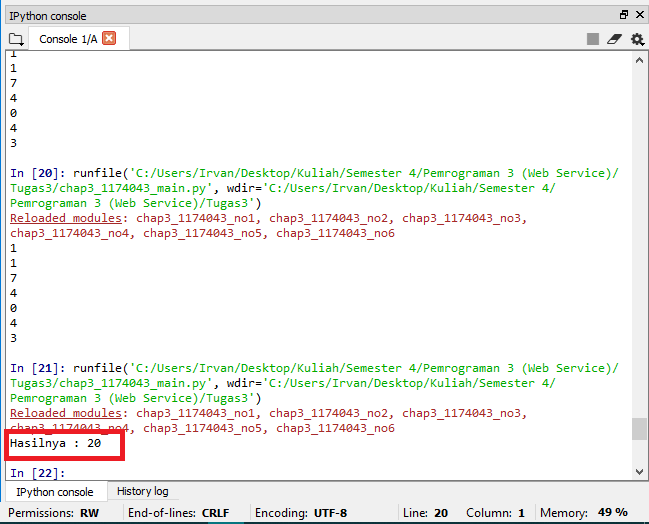
\includegraphics[width=1\textwidth]{figures/chapter3/6_1174043.png}}
					\caption{Jawaban No. 6}
					\label{6}
				\end{figure}

				\ref{6_1174043}
				
			\item Jawaban soal no 7
				\lstinputlisting{src/chapter3/chap3_1174043_no7.py}
				
				\begin{figure} [ht]
					\centerline{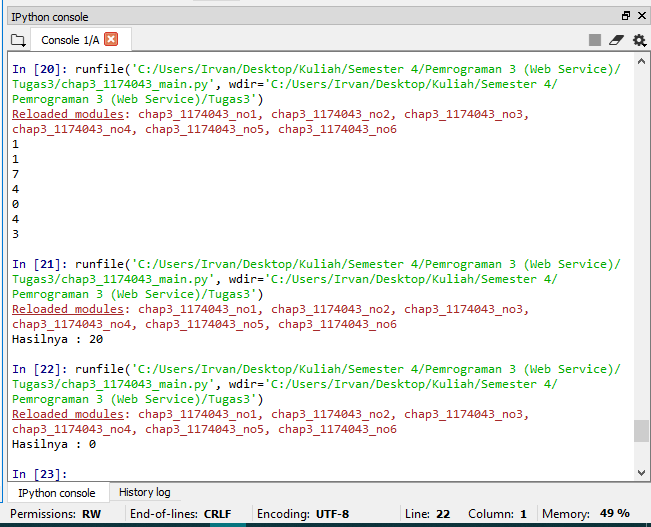
\includegraphics[width=1\textwidth]{figures/chapter3/7_1174043.png}}
					\caption{Jawaban No. 7}
					\label{7}
				\end{figure}

				\ref{7_1174043}
				
			\item Jawaban soal no 8
				\lstinputlisting{src/chapter3/chap3_1174043_no8.py}
				
				\begin{figure} [ht]
					\centerline{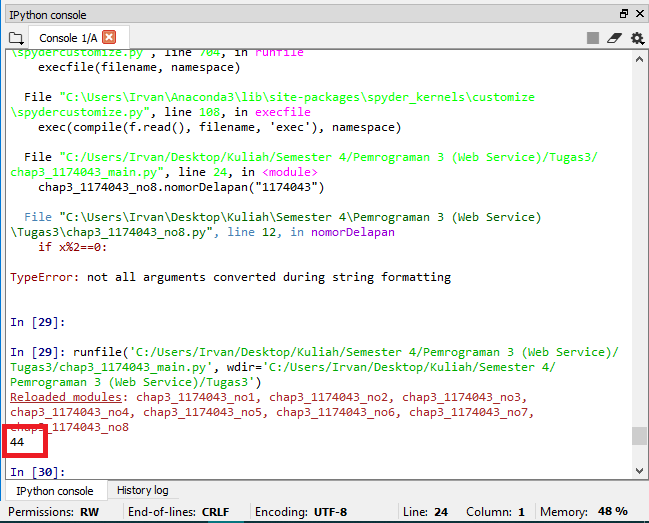
\includegraphics[width=1\textwidth]{figures/chapter3/8_1174043.png}}
					\caption{Jawaban No. 8}
					\label{8}
				\end{figure}

				\ref{8_1174043}
				
			\item Jawaban soal no 9
				\lstinputlisting{src/chapter3/chap3_1174043_no9.py}
				
				\begin{figure} [ht]
					\centerline{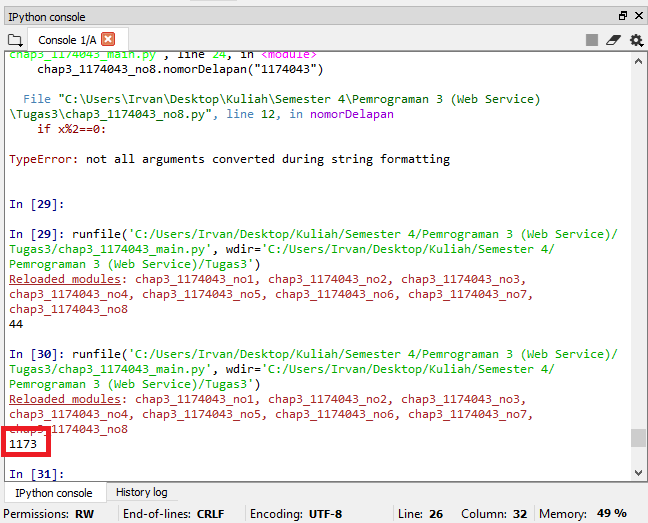
\includegraphics[width=1\textwidth]{figures/chapter3/9_1174043.png}}
					\caption{Jawaban No. 9}
					\label{9}
				\end{figure}

				\ref{9_1174043}
				
			\item Jawaban soal no 10
				\lstinputlisting{src/chapter3/chap3_1174043_no10.py}
				
				\begin{figure} [ht]
					\centerline{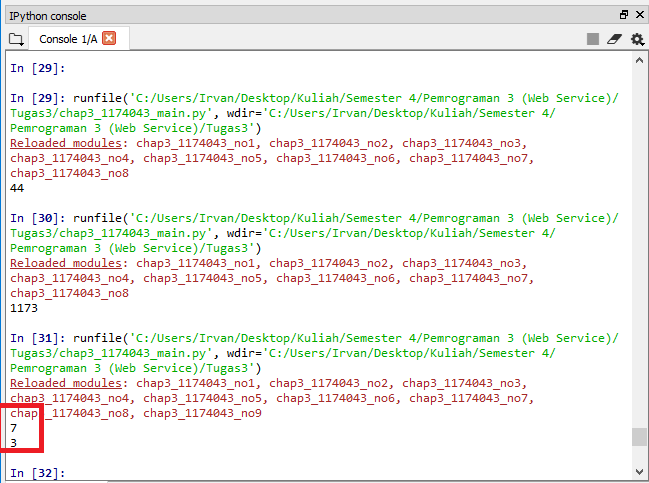
\includegraphics[width=1\textwidth]{figures/chapter3/10_1174043.png}}
					\caption{Jawaban No. 10}
					\label{10}
				\end{figure}

				\ref{10_1174043}
				
			\item Jawaban soal no 11
			
				File 3lib.py
				\lstinputlisting{src/chapter3/chap3_1174043_3lib.py}
				
				File main.py
				\lstinputlisting{src/chapter3/chap3_1174043_main.py}
				
				\begin{figure} [ht]
					\centerline{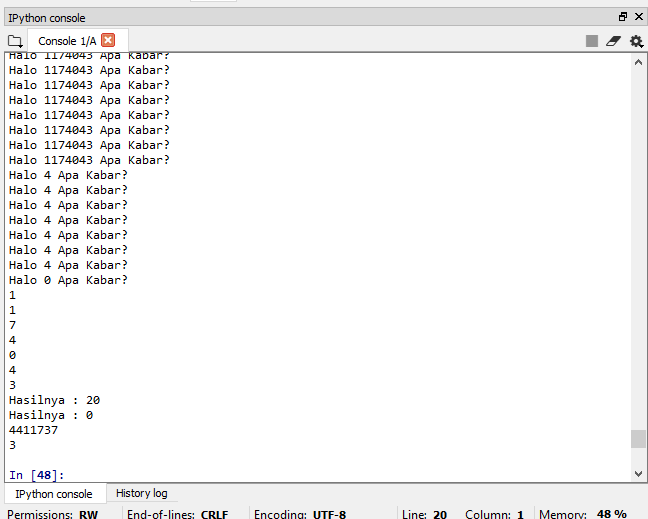
\includegraphics[width=1\textwidth]{figures/chapter3/11_1174043.png}}
					\caption{Jawaban No. 11}
					\label{11}
				\end{figure}

				\ref{11_1174043}
				
			\item Jawaban soal no 12
			\lstinputlisting{src/chapter3/chap3_1174043_kelas3lib.py}
		
		\end{enumerate}
		
		\subsection{Keterampilan Penanganan Error}
			\begin{enumerate}
				\item \lstinputlisting{src/chapter3/chap3_1174043_3err.py}
			
			\end{enumerate}
			
		\subsection{Plagiarisme}
			\begin{figure} [ht]
					\centerline{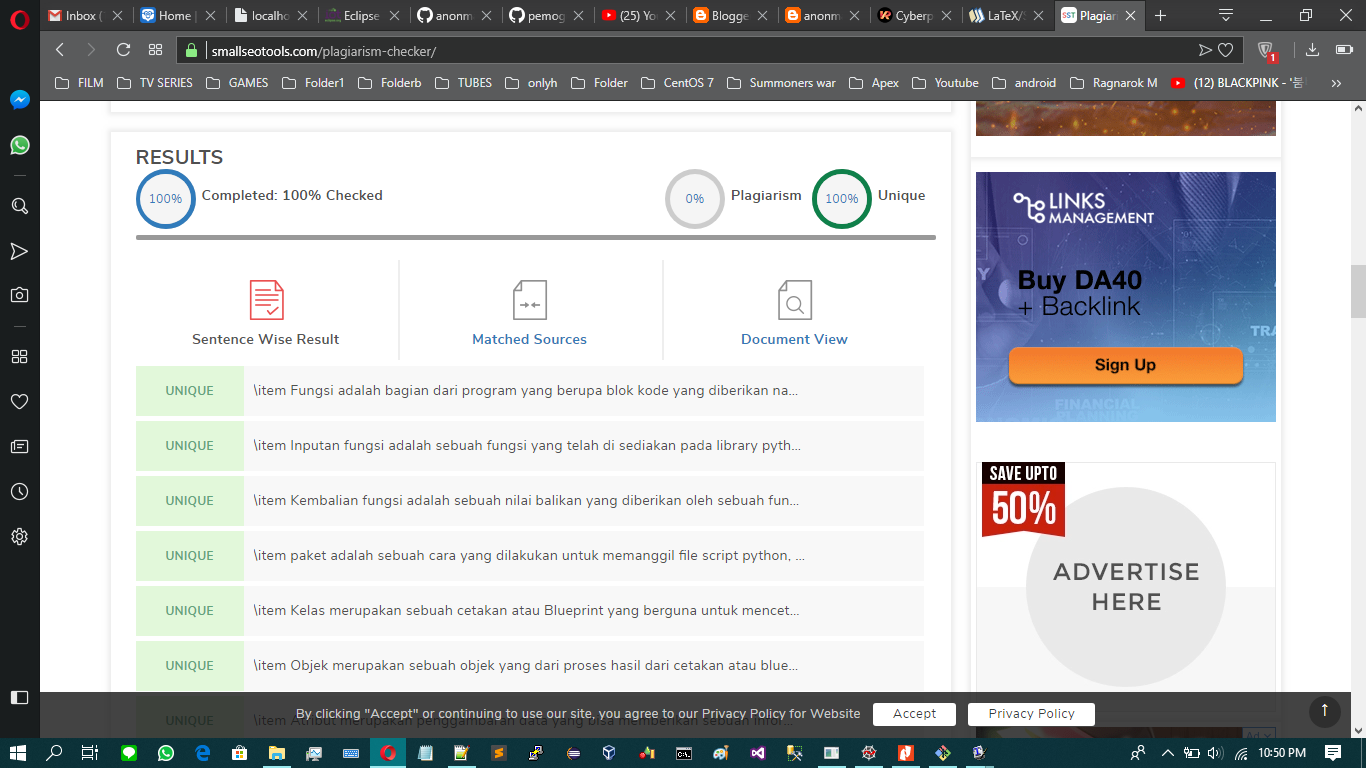
\includegraphics[width=1\textwidth]{figures/chapter3/plagiarisme_1174043.png}}
					\caption{Hasil Cek Plagiarisme}
					\label{plagiarisme}
				\end{figure}

			\ref{plagiarisme_1174043}

\subsection{Luthfi Muhammad Nabil/1174035}
\subsubsection{Pemahaman Teori}
\begin{enumerate}
	\item Fungsi adalah sintaks yang terdiri dari nama fungsi, parameter input variabel, dan variabel kembali. Pada python, nama fungsi diawali dengan def dan pada sintaks paling akhir (setelah parameter) adalah titik dua. Aturan penamaan dari fungsi sama dengan penamaan sebuah variabel yang salah satunya yaitu case sensitive. Untuk penulisan parameter tidak harus memasukan inputan dan batas untuk penulisan variabel pada parameter tidak memiliki batas atau bisa lebih dari satu dengan pemisah tanda koma. Nilai yang dapat dikembalikan oleh fungsi dapat berupa variabel yang mau dikembalikan. Berikut contoh dari koding fungsi : 
	\lstinputlisting[firstline=1, lastline=4]{src/chapter3/chap3_1174035_teori.py}
	\item Paket merupakan sebuah file yang berisikan fungsi - fungsi yang dapat dipakai. Untuk pemanggilan fungsi diperlukan keyword import untuk memanggil paket tersebut. berikut contoh pemakaian dari paket : 
	\lstinputlisting[firstline=6, lastline=8]{src/chapter3/chap3_1174035_teori.py}
	\item Class merupakan cetak biru dari sebuah objek yang dibuat. Objek merupakan instansi dari sebuah class. Atribut merupakan variabel atau yang menampung nilai pada sebuah objek. Fungsi adalah sebuah pembungkus kumpulan instruksi pada sebuah program. Berikut contohnya : 
	\lstinputlisting[firstline=10, lastline=24]{src/chapter3/chap3_1174035_teori.py}
	\item Pemanggilan sebuah kelas diawali dari sebuah paket dipanggil terlebih dahulu, lalu kelas akan disimpan ke variabel untuk diinisiasi sebagai objek. Berikut contoh pemanggilan dari kelas : 
	\lstinputlisting[firstline=26, lastline=29]{src/chapter3/chap3_1174035_teori.py}
	\item Pemakaian from kalkulator merupakan sebuah inisiasi untuk memanggil fungsi penambahan dari paket kalkulator yang dipanggil agar fungsi penambahandapat digunakan langsung tanpa menulis nama file dari paket yaitu kalkulator. Berikut Contohnya : 
	\lstinputlisting[firstline=31, lastline=34]{src/chapter3/chap3_1174035_teori.py}
	\item Pemakaian paket fungsi memanggil fungsi dari paket lain dan memanggil paket tersebut dengan tambahan nama asal paket dari fungsi yang akan dipanggil. Berikut pemakaiannya : 
	\lstinputlisting[firstline=36, lastline=39]{src/chapter3/chap3_1174035_teori.py}
	\item Pemakaian paket kelas sama halnya dengan fungsi hanya saja untuk paket kelas diinisiasikan terlebih dahulu lalu nilai variabel akan dikirim ke constructor dari class tersebut. Pada saat memanggil fungsi tidak perlu menggunakan inputan parameter karena nilai yang dikirim sudah disimpan pada constructor di class yang dipanggil. Berikut Contohnya : 
	\lstinputlisting[firstline=41, lastline=46]{src/chapter3/chap3_1174035_teori.py}
\end{enumerate}
\subsection{Ketrampilan Pemrograman}
\begin{enumerate}
	\item Membuat fungsi dengan inputan variabel NPM, dan melakukan print luaran huruf yang dirangkai dari tanda bintang, paga,r, plus dari NPM kita. Untuk NPM mod 3=0 memakai bintang, NPM mod 3=1 memakai pagar, NPM mod 3 = 2 memakai tanda plus. Kodingnya : 
	\lstinputlisting{src/chapter3/chap3_1174035_1.py}
	\begin{figure}[!htbp]
        \centering
        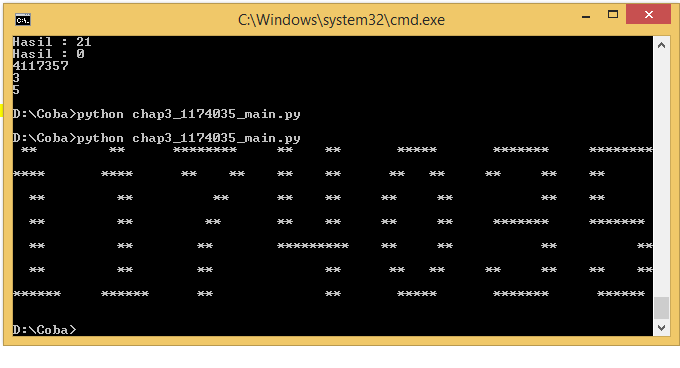
\includegraphics[height=7cm, width=10cm]{figures/chapter3/1174035_1.png}
        \caption{Screenshot No 1}
        \label{1174035_1}
	\end{figure}
	\item Membuat fungsi dengan inputan variabel NPM, dan lakukan perulangan untuk mengeluarkan print output sebanyak dua dijit belakang NPM. Contoh NPM : 1174035 maka akan ada output sebanyak 35 kali dengan tulisan 'Hallo, 1174035 apa kabar?' Kodingnya : 
	\lstinputlisting{src/chapter3/chap3_1174035_2.py}
	\begin{figure}[!htbp]
        \centering
        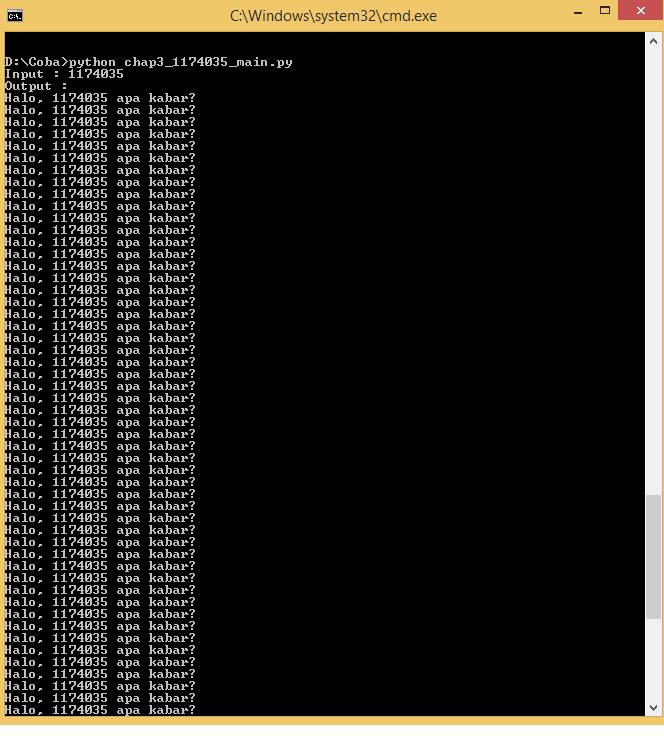
\includegraphics[height=7cm, width=10cm]{figures/chapter3/1174035_2.png}
        \caption{Screenshot No 2}
        \label{1174035_2}
	\end{figure}
	\item Membuat fungsi dengan inputan variabel NPM, dan melakukan print luaran output dengan perulangan berupa tiga karakter belakang dari NPM dijumlahkan. Lalu jumah perulangan tersebut adalah total dari tiga karakter belakang NPM dijumlahkan. Kodingnya : 
	\lstinputlisting{src/chapter3/chap3_1174035_3.py}
	\begin{figure}[!htbp]
        \centering
        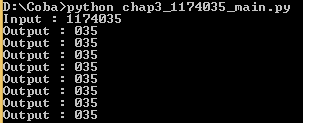
\includegraphics[height=7cm, width=10cm]{figures/chapter3/1174035_3.png}
        \caption{Screenshot No 3}
        \label{1174035_3}
	\end{figure}
	\item Membuat fungsi dengan inputan variabel NPM, dan melakukan print hello world dan digit ketiga dari belakang dari NPM. contoh : NPM : 0, Output : Halo, 0 apa kabar? .Kodingnya : 
	\lstinputlisting{src/chapter3/chap3_1174035_4.py}
	\begin{figure}[!htbp]
        \centering
        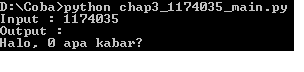
\includegraphics[height=3cm, width=8cm]{figures/chapter3/1174035_4.png}
        \caption{Screenshot No 4}
        \label{1174035_4}
	\end{figure}
	\item Membuat fungsi dengan inputan variabel NPM, dan menampilkan semua angka dari NPM tersebut secara berurutan kebawah. Kodingnya : 
	\lstinputlisting{src/chapter3/chap3_1174035_5.py}
	\begin{figure}[!htbp]
        \centering
        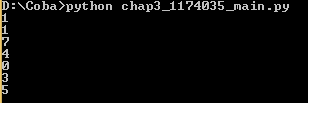
\includegraphics[height=5cm, width=10cm]{figures/chapter3/1174035_5.png}
        \caption{Screenshot No 5}
        \label{1174035_5}
	\end{figure}
	\item Membuat fungsi dengan inputan variabel NPM, didalamnya melakukan penjumlahan dari seluruh dijit NPM tersebut. menggunakan perulangan atau kondisi. Kodingnya : 
	\lstinputlisting{src/chapter3/chap3_1174035_6.py}
	\begin{figure}[!htbp]
        \centering
        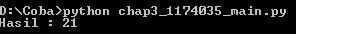
\includegraphics[height=5cm, width=10cm]{figures/chapter3/1174035_6.png}
        \caption{Screenshot No 6}
        \label{1174035_6}
	\end{figure}
	\item Membuat fungsi dengan inputan variabel NPM, didalamnya melakukan perkalian dari seluruh dijit NPM tersebut. menggunakan perulangan atau kondisi. Kodingnya : 
	\lstinputlisting{src/chapter3/chap3_1174035_7.py}
	\begin{figure}[!htbp]
        \centering
        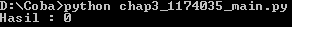
\includegraphics[height=4cm, width=10cm]{figures/chapter3/1174035_7.png}
        \caption{Screenshot No 7}
        \label{1174035_7}
	\end{figure}
	\item Membuat fungsi dengan inputan variabel NPM, lalu lakukan print seluruh angka genap dari setiap angka di NPM. Kodingnya : 
	\lstinputlisting{src/chapter3/chap3_1174035_8.py}
	\begin{figure}[!htbp]
        \centering
        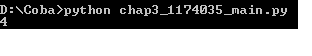
\includegraphics[height=4cm, width=10cm]{figures/chapter3/1174035_8.png}
        \caption{Screenshot No 8}
        \label{1174035_8}
	\end{figure}
	\item Membuat fungsi dengan inputan variabel NPM, lalu lakukan print seluruh angka ganjil dari setiap angka di NPM. Kodingnya : 
	\lstinputlisting{src/chapter3/chap3_1174035_9.py}
	\begin{figure}[!htbp]
        \centering
        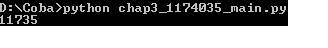
\includegraphics[height=4cm, width=10cm]{figures/chapter3/1174035_9.png}
        \caption{Screenshot No 9}
        \label{1174035_9}
	\end{figure}
	\item Membuat fungsi dengan inputan variabel NPM, lalu lakukan print seluruh angka prima dari setiap angka di NPM. Kodingnya : 
	\lstinputlisting{src/chapter3/chap3_1174035_10.py}
	\begin{figure}[!htbp]
        \centering
        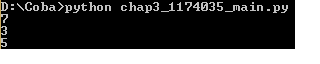
\includegraphics[height=5cm, width=10cm]{figures/chapter3/1174035_10.png}
        \caption{Screenshot No 10}
        \label{1174035_10}
	\end{figure}
	\item Membuat Satu File library bernama 3lib.py yang berisi semua fungsi - fungsi dari setiap nomor pada soal praktek. Kodingnya : 	
	\lstinputlisting{src/chapter3/chap3_1174035_3lib.py}
	\lstinputlisting[firstline=1, lastline=15]{src/chapter3/chap3_1174035_main.py}
	
	\begin{figure}[!htbp]
        \centering
        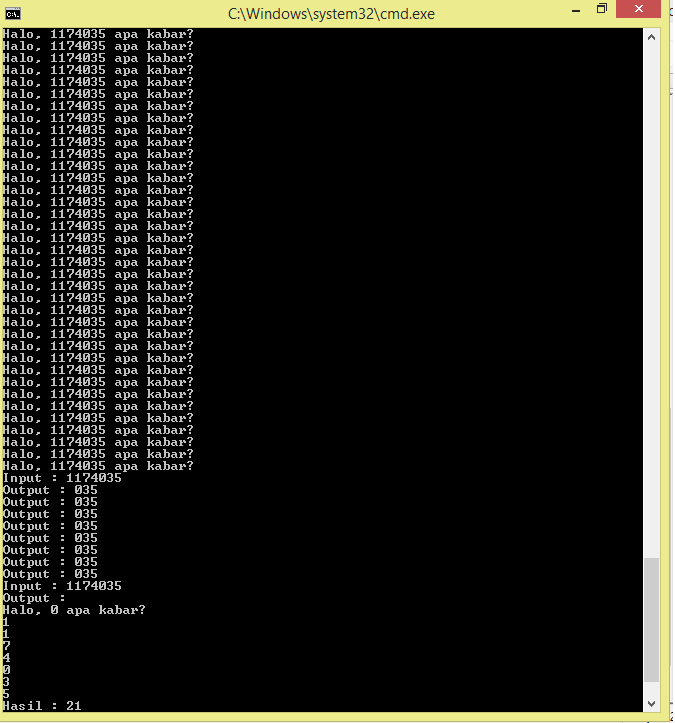
\includegraphics[height=10cm, width=8cm]{figures/chapter3/1174035_3lib.png}
        \caption{Screenshot No 11}
        \label{1174035_3lib}
	\end{figure}
	
	\item Membuat Satu File library bernama kelas3lib.py yang berisi kelas yang isinya semua fungsi - fungsi dari setiap nomor yang telah dimodifikasi untuk menyesuaikan dengan kelas. Kodingnya : 	
	\lstinputlisting{src/chapter3/chap3_1174035_kelas3lib.py}
	\lstinputlisting[firstline=16, lastline=29]{src/chapter3/chap3_1174035_main.py}
	
	\begin{figure}[!htbp]
        \centering
        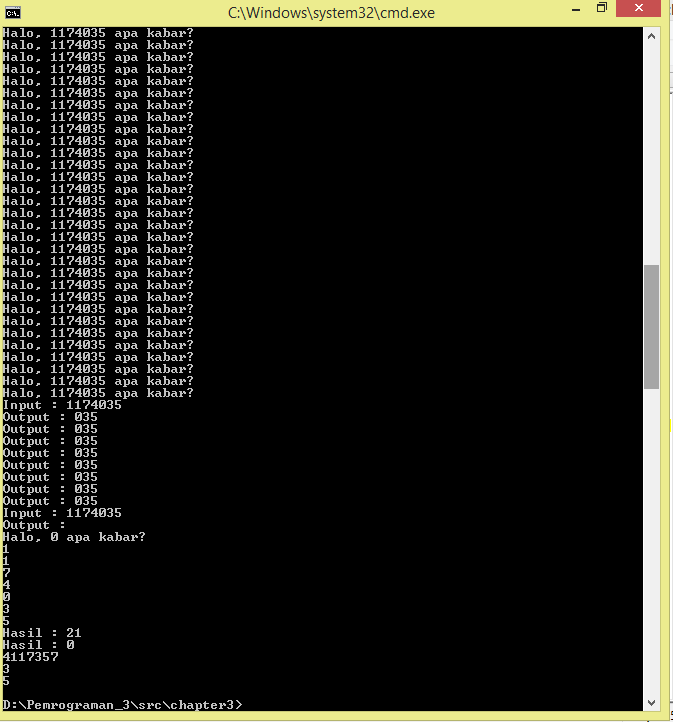
\includegraphics[height=10cm, width=8cm]{figures/chapter3/1174035_kelas3lib.png}
        \caption{Screenshot No 12}
        \label{1174035_kelas3lib}
	\end{figure}
	
	
\end{enumerate}

\subsubsection{Error}
\begin{enumerate}
	\item Tuliskan error yang terjadi saat mengerjakan section ini. Mendapat error yaitu salah konversi. Untuk menghandle error tersebut dapat menggunakan try catch :
	\lstinputlisting{src/chapter3/chap3_1174035_error.py}
	\lstinputlisting[firstline=32, lastline=36]{src/chapter3/chap3_1174035_main.py}
	\begin{figure}[!htbp]
        \centering
        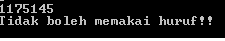
\includegraphics[height=3cm, width=8cm]{figures/chapter3/1174035_error.png}
        \caption{Screenshot No 13}
        \label{1174035_error}
	\end{figure}
	\item Plagiarisme
	\begin{figure}[!htbp]
        \centering
        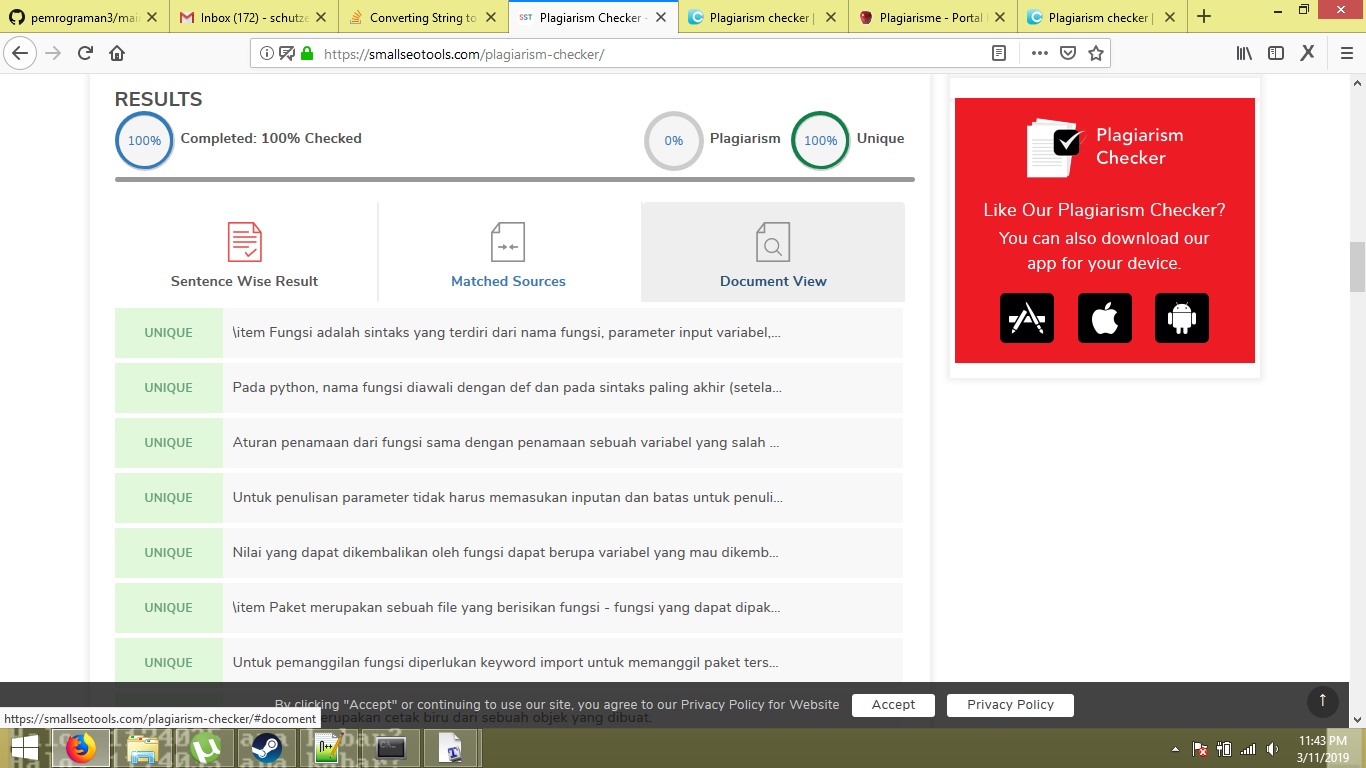
\includegraphics[height=7cm, width=9cm]{figures/chapter3/1174035_plagiarisme.png}
        \caption{Plagiarisme}
        \label{1174035_plagiarisme}
	\end{figure}
\end{enumerate}

\section{Rangga Putra Ramdhani}
\subsubsection{Pemahanan Teori}
\begin{enumerate}
    \item Apa itu fungsi, inputan fungsi dan kembalian fungsi dengan contoh kode program
    lainnya.
    Fungsi adalah bagian dari program yang dapat digunakan ulang.
    Berikut merupakan contoh fungsi dan cara pemanggilannya
    \lstinputlisting[firstline=124, lastline=127]{src/1174056_praktek.py}

    Fungsi dapat membaca parameter, parameter adalah nilai yang disediakan kepada fungsi, dimana nilai ini akan menentukan output yang akan dihasilkan fungsi.
    \lstinputlisting[firstline=129, lastline=132]{src/1174056_praktek.py}

    Statemen return digunakan untuk keluar dari fungsi. Kita juga dapat menspesifikasikan nilai kembalian.
    \lstinputlisting[firstline=134, lastline=141]{src/1174056_praktek.py}

    \item Apa itu paket dan cara pemanggilan paket atau library dengan contoh kode
    program lainnya.
    Untuk memudahkan dalam pemanggilan fungsi yang di butuhkan, agar dapat dipanggil berulang.
    Cara pemanggilannya
    \lstinputlisting[firstline=143, lastline=144]{src/1174056_praktek.py}

    \item Jelaskan Apa itu kelas, apa itu objek, apa itu atribut, apa itu method dan
    contoh kode program lainnya masing-masing.
    kelas merupakan sebuah blueprint yang mepresentasikan objek.
    objek adalah hasil cetakan dadri sebuah kelas.
    method adalah suatu upaya yang digunakan oleh object.
    \lstinputlisting[firstline=146, lastline=168]{src/1174056_praktek.py}

    \item Jelaskan cara pemanggikan library kelas dari instansiasi dan pemakaiannya den-
    gan contoh program lainnya.
    Cara Pemanggilanya 
    \begin{itemize}
        \item pertama import terlebih dahulu filenya.
        \item kemudian buat variabel untuk menampung datanya
        \item setelah itu panggil nama classnya dan panggil methodnya
        \item Gunakan perintah print untuk menampilkan hasilnya

    \end{itemize}
    \lstinputlisting[firstline=170, lastline=175]{src/1174056_praktek.py}

    \item Jelaskan dengan contoh pemakaian paket dengan perintah from kalkulator im-
    port Penambahan disertai dengan contoh kode lainnya.
    Penggunaan paket from namafile import, itu berfungsi untuk memanggil file dan fungsinya
    \lstinputlisting[firstline=143, lastline=144]{src/1174056_praktek.py}

    \item Jelaskan dengan contoh kodenya, pemakaian paket fungsi apabila le library
    ada di dalam folder.
    Pemakaian paket adalah perkumpulan fungsi-fungsi. contoh kodenya adalah sebagai berikut :

    \item Jelaskan dengan contoh kodenya, pemakaian paket kelas apabila le library ada
    di dalam folder.
    \lstinputlisting[firstline=184, lastline=184]{src/1174056_praktek.py}

\end{enumerate}
\subsubsection{Ketrampilan Pemrograman}
\begin{enumerate}
    \item Buatlah fungsi dengan inputan variabel NPM, dan melakukan print luaran huruf
    yang dirangkai dari tanda bintang, pagar atau plus dari NPM kita. Tanda
    bintang untuk NPM mod 3=0, tanda pagar untuk NPM mod 3 =1, tanda plus
    untuk NPM mod3=2.
    \lstinputlisting[firstline=184, lastline=234]{src/1174056_praktek.py}

    \item Buatlah fungsi dengan inputan variabel berupa NPM. kemudian dengan meng-
    gunakan perulangan mengeluarkan print output sebanyak dua dijit belakang
    NPM.
    \lstinputlisting[firstline=237, lastline=243]{src/1174056_praktek.py}

    \item Buatlah fungsi dengan dengan input variabel string bernama NPM dan beri
    luaran output dengan perulangan berupa tiga karakter belakang dari NPM se-
    banyak penjumlahan tiga dijit tersebut.
    \lstinputlisting[firstline=245, lastline=255]{src/1174056_praktek.py}

    \item Buatlah fungsi hello word dengan input variabel string bernama NPM dan
    beri luaran output berupa digit ketiga dari belakang dari variabel NPM meng-
    gunakan akses langsung manipulasi string pada baris ketiga dari variabel NPM.
    \lstinputlisting[firstline=257, lastline=263]{src/1174056_praktek.py}

    \item buat fungsi program dengan input variabel NPM dan melakukan print nomor npm satu persatu kebawah.
    \lstinputlisting[firstline=265, lastline=269]{src/1174056_praktek.py}

    \item Buatlah fungsi dengan inputan variabel NPM, didalamnya melakukan penjum-
    lahan dari seluruh dijit NPM tersebut, wajib menggunakan perulangan dan
    atau kondisi.
    \lstinputlisting[firstline=272, lastline=279]{src/1174056_praktek.py}

    \item Buatlah fungsi dengan inputan variabel NPM, didalamnya melakukan melakukan
    perkalian dari seluruh dijit NPM tersebut, wajib menggunakan perulangan dan
    atau kondisi.
    \lstinputlisting[firstline=281, lastline=288]{src/1174056_praktek.py}

    \item Buatlah fungsi dengan inputan variabel NPM, Lakukan print NPM anda tapi
    hanya dijit genap saja. wajib menggunakan perulangan dan atau kondisi.
    \lstinputlisting[firstline=290, lastline=296]{src/1174056_praktek.py}

    \item Buatlah fungsi dengan inputan variabel NPM, Lakukan print NPM anda tapi
    hanya dijit ganjil saja. wajib menggunakan perulangan dan atau kondisi.
    \lstinputlisting[firstline=298, lastline=304]{src/1174056_praktek.py}

    \item Buatlah fungsi dengan inputan variabel NPM, Lakukan print NPM anda tapi
    hanya dijit yang termasuk bilangan prima saja. wajib menggunakan perulangan
    dan atau kondisi.
    \lstinputlisting[firstline=306, lastline=320]{src/1174056_praktek.py}

    \item Buatlah satu library yang berisi fungsi-fungsi dari nomor diatas dengan nama
    le rangga.py dan berikan contoh cara pemanggilannya pada le main.py.
    \lstinputlisting[firstline=7, lastline=7]{src/mainn.py}

    \item Buatlah satu library class dengan nama le kelas3lib.py yang merupakan mod-
    ikasi dari fungsi-fungsi nomor diatas dan berikan contoh cara pemanggilannya
    pada le mainn.py.
    \lstinputlisting[firstline=8, lastline=9]{src/mainn.py}
    
\end{enumerate}
\subsubsection{Ketrampilan Penanganan Error}
Error yang di dapat dari mengerjakan tugas ini adalah type error, cara menaggulaginya dengan cara mengecheck kembali codingannya
kemudian run kembali aplikasinya
berikut contoh Penggunaan fungsi try dan exception
\lstinputlisting[firstline=177, lastline=182]{src/1174056_praktek.py}


\section{Faisal Najib Abdullah}
\subsection{Pemahanan Teori}
\begin{enumerate}
    \item Apa itu fungsi, inputan fungsi dan kembalian fungsi dengan contoh kode program
    lainnya.
    Fungsi adalah bagian dari program yang dapat digunakan ulang.
    Berikut merupakan contoh fungsi dan cara pemanggilannya
    \lstinputlisting{src/chapter3/1174042_1,1.py}

    Fungsi dapat membaca parameter, parameter adalah nilai yang disediakan kepada fungsi, dimana nilai ini akan menentukan output yang akan dihasilkan fungsi.
    \lstinputlisting{src/chapter3/1174042_1,1,1.py}

    Statemen return digunakan untuk keluar dari fungsi. Kita juga dapat menspesifikasikan nilai kembalian.
    \lstinputlisting{src/chapter3/1174042_1,1,2.py}

    \item Apa itu paket dan cara pemanggilan paket atau library dengan contoh kode
    program lainnya.
    Untuk memudahkan dalam pemanggilan fungsi yang di butuhkan, agar dapat dipanggil berulang.
    Cara pemanggilannya
    \lstinputlisting{src/chapter3/1174042_1,2.py}

    \item Jelaskan Apa itu kelas, apa itu objek, apa itu atribut, apa itu method dan
    contoh kode program lainnya masing-masing.
    kelas merupakan sebuah blueprint yang mepresentasikan objek.
    objek adalah hasil cetakan dadri sebuah kelas.
    method adalah suatu upaya yang digunakan oleh object.
    \lstinputlisting{src/chapter3/1174042_1,3.py}

    \item Jelaskan cara pemanggikan library kelas dari instansiasi dan pemakaiannya den-
    gan contoh program lainnya.
    Cara Pemanggilanya 
    \begin{itemize}
        \item pertama import terlebih dahulu filenya.
        \item kemudian buat variabel untuk menampung datanya
        \item setelah itu panggil nama classnya dan panggil methodnya
        \item Gunakan perintah print untuk menampilkan hasilnya

    \end{itemize}
    \lstinputlisting{src/chapter3/1174042_1,4.py}

    \item Jelaskan dengan contoh pemakaian paket dengan perintah from kalkulator im-
    port Penambahan disertai dengan contoh kode lainnya.
    Penggunaan paket from namafile import, itu berfungsi untuk memanggil file dan fungsinya
    \lstinputlisting{src/chapter3/1174042_1,2.py}

    \item Jelaskan dengan contoh kodenya, pemakaian paket fungsi apabila file library
    ada di dalam folder.
    Pemakaian paket adalah perkumpulan fungsi-fungsi. contoh kodenya adalah sebagai berikut :
	\lstinputlisting{src/chapter3/1174042_1,6.py}

    \item Jelaskan dengan contoh kodenya, pemakaian paket kelas apabila file library ada
    di dalam folder.
    \lstinputlisting{src/chapter3/1174042_1,6.py}

	\end{enumerate}

\subsection{Ketrampilan Pemrograman}
\begin{enumerate}
    \item Buatlah fungsi dengan inputan variabel NPM, dan melakukan print luaran huruf
    yang dirangkai dari tanda bintang, pagar atau plus dari NPM kita. Tanda
    bintang untuk NPM mod 3=0, tanda pagar untuk NPM mod 3 =1, tanda plus
    untuk NPM mod3=2.
    \lstinputlisting{src/chapter3/1174042_2,1.py}

    \item Buatlah fungsi dengan inputan variabel berupa NPM. kemudian dengan meng-
    gunakan perulangan mengeluarkan print output sebanyak dua dijit belakang
    NPM.
    \lstinputlisting{src/chapter3/1174042_2,2.py}

    \item Buatlah fungsi dengan dengan input variabel string bernama NPM dan beri
    luaran output dengan perulangan berupa tiga karakter belakang dari NPM se-
    banyak penjumlahan tiga dijit tersebut.
    \lstinputlisting{src/chapter3/1174042_2,3.py}

    \item Buatlah fungsi hello word dengan input variabel string bernama NPM dan
    beri luaran output berupa digit ketiga dari belakang dari variabel NPM meng-
    gunakan akses langsung manipulasi string pada baris ketiga dari variabel NPM.
    \lstinputlisting{src/chapter3/1174042_2,4.py}

    \item buat fungsi program dengan input variabel NPM dan melakukan print nomor npm satu persatu kebawah.
    \lstinputlisting{src/chapter3/1174042_2,5.py}

    \item Buatlah fungsi dengan inputan variabel NPM, didalamnya melakukan penjum-
    lahan dari seluruh dijit NPM tersebut, wajib menggunakan perulangan dan
    atau kondisi.
    \lstinputlisting{src/chapter3/1174042_2,6.py}

    \item Buatlah fungsi dengan inputan variabel NPM, didalamnya melakukan melakukan
    perkalian dari seluruh dijit NPM tersebut, wajib menggunakan perulangan dan
    atau kondisi.
    \lstinputlisting{src/chapter3/1174042_2,7.py}

    \item Buatlah fungsi dengan inputan variabel NPM, Lakukan print NPM anda tapi
    hanya dijit genap saja. wajib menggunakan perulangan dan atau kondisi.
    \lstinputlisting{src/chapter3/1174042_2,8.py}

    \item Buatlah fungsi dengan inputan variabel NPM, Lakukan print NPM anda tapi
    hanya dijit ganjil saja. wajib menggunakan perulangan dan atau kondisi.
    \lstinputlisting{src/chapter3/1174042_2,9.py}

    \item Buatlah fungsi dengan inputan variabel NPM, Lakukan print NPM anda tapi
    hanya dijit yang termasuk bilangan prima saja. wajib menggunakan perulangan
    dan atau kondisi.
    \lstinputlisting{src/chapter3/1174042_2,10.py}

    \item Buatlah satu library yang berisi fungsi-fungsi dari nomor diatas dengan nama
    file 3lib.py dan berikan contoh cara pemanggilannya pada file main.py.
    \lstinputlisting{src/chapter3/1174042_main.py}

    \item Buatlah satu library class dengan nama file kelas3lib.py yang merupakan mod-
    ifikasi dari fungsi-fungsi nomor diatas dan berikan contoh cara pemanggilannya
    pada file main.py.
    \lstinputlisting{src/chapter3/1174042_main.py}
    
\end{enumerate}
\subsection{Ketrampilan Penanganan Error}
Error yang di dapat dari mengerjakan tugas ini adalah type error, cara menaggulaginya dengan cara mengecheck kembali codingannya
kemudian run kembali aplikasinya
berikut contoh Penggunaan fungsi try dan exception
\lstinputlisting{src/chapter3/1174042_2err.py}

\section{Yusniar Nur Syarif Sidiq/1164089}
\subsection{Teori}
\begin{enumerate}
\item Fungsi merupakan sebuah bagian dari program yang dapat digunakan ulang dan memiliki inputan variabel serta nilai yang akan di kembalikannya. Contohnya adalah source code berikut ini,
	 \lstinputlisting{src/chapter2/1164089/1164089_1.py}
Dalam dalam source code tersebut akan mengeluarkan output Hallo 1164089 ketika kita running di dalam spyder.

\item Library dalam python disini merupakan kumpulan dari fungsi dan cara pemanggilannya adalah dengan melakukan import file librarynya. Sebagai contoh, buatlah Matematika.py dan 1164089\_2.py, simpan dalam satu folder. Untuk Matematika.py isikan fungsi sebagai berikut
	 \lstinputlisting{src/chapter2/1164089/Matematika.py}
Untuk memanggil fungsi tersebut adalah dengan melakukan import  Matematika.py pada 1164089\_2.py adalah sebagai berikut,
	 \lstinputlisting{src/chapter2/1164089/1164089_2.py}

\item Class merupakan salah satu cara untuk membuat sebuah kode yang mempunyai objek serta atribut tertentu sehingga akan lebih mudah dalam mengorganisasi berbagai fungsi dan statenya. Objek disini merupakan instansiasi atau perwujudan dari sebuah class. Untuk membuat class yang memiliki objek serta atribut dapat dilihat pada source code berikut ini, dimana kita akan membaut file bernama mtk.py
	\lstinputlisting{src/chapter2/1164089/mtk.py}
Self tersebut berfungsi untuk menunjukkan variabel lokal dari class tersebut. Untuk memanggil class tersebut kita akan membuat file bernama 1164089\_3.py dan kita akan melakukan import mtk.py pada file tersebut, untuk source codenya dapat dilihat seperti berikut,
	\lstinputlisting{src/chapter2/1164089/1164089_3.py}

\item Cara memanggilnya yaitu
	\begin{itemize}
		\item Pertama import terlebih dahulu filenya
		\item Buat variabel yang berfungsi menampung data
		\item Panggil nama classnya dan methodnya
		\item Gunakan perintah print untuk menampilkannya
	\end{itemize}
Sebagai contoh perhatikan source code ini,
	\lstinputlisting{src/chapter2/1164089/1164089_4.py}

\item Dimana kita akan melakukan membuka library Matematika.py dan akan melakukan import dari fungsi di dalamnya yaitu matematika, sehingga akan lebih simple dalam penulisan source codenya adalah sebagai berikut,
	\lstinputlisting{src/chapter2/1164089/1164089_5.py}

\item

\item 
\end{enumerate}

\subsection{Keterampilan Pemrograman}
\begin{enumerate}

\item Soal No 1 \lstinputlisting{src/chapter2/1164089/1164089_21.py}

\item Soal No 2 \lstinputlisting{src/chapter2/1164089/1164089_22.py}

\item Soal No 3 \lstinputlisting{src/chapter2/1164089/1164089_23.py}

\item Soal No 4 \lstinputlisting{src/chapter2/1164089/1164089_24.py}

\item Soal No 5 \lstinputlisting{src/chapter2/1164089/1164089_25.py}

\item Soal No 6 \lstinputlisting{src/chapter2/1164089/1164089_26.py}

\item Soal No 7 \lstinputlisting{src/chapter2/1164089/1164089_27.py}

\item Soal No 8 \lstinputlisting{src/chapter2/1164089/1164089_28.py}

\item Soal No 9 \lstinputlisting{src/chapter2/1164089/1164089_29.py}

\item Soal No 10 \lstinputlisting{src/chapter2/1164089/1164089_30.py}

\item Soal No 11 \lstinputlisting{src/chapter2/1164089/1164089_31.py}

\item Soal No 12 \lstinputlisting{src/chapter2/1164089/1164089_32.py}
\end{enumerate}

\subsection{Penanganan Erorr}
\begin{enumerate}

\item Erorr yang saya temui di antaranya adalah Systax Erorr, dimana suatu keadaan script python mengalami kesalahan dalam penulisannya dan solusi dari permasalahan ini adalah dengan memperbaiki script penulisan yang salah. Untuk contoh fungsi trx except dapat dilihat pada source code berikut ini,

	\lstinputlisting{src/chapter2/1164089/1164089_33.py}

\end{enumerate}

\section{Fathi Rabbani/1164074/3C}
\subsection{Teori}
\begin{enumerate}
\item Fungsi, Inputan dan Return
	\begin{itemize}
	\item Fungsi adalah sebuah blok code yang digunakan untuk melempar parameter kedalam blok code yang berbeda.
		\lstinputlisting[firstline=9, lastline=11]{src/chapter3/1164074/praktek.py}
	\item Inputan fungsi adalah sebuah fungsi yang memiliki parameter berupa inputan atau data yang bias diinputkan.
		\lstinputlisting[firstline=13, lastline=15]{src/chapter3/1164074/praktek.py}
	\item Pengembalian fungsi atau sering juga disebut sebagai return merupakan sebuah pengembalian nilai dari pengeksekusian data pada parameter yang terdapat difungsi.
		\lstinputlisting[firstline=17, lastline=24]{src/chapter3/1164074/praktek.py}
	\end{itemize}

\item Paket atau Library Fungsi
	\subitem paket merupakan sebuah penggunaan library dengan maksud mempermudah dalam eksekusi dan pemanggilan fungsi
		\lstinputlisting[firstline=171, lastline=173]{src/chapter3/1164074/praktek.py}
	berikut ini adalah fungsi yang digunakan untuk memanggil paket atau library
		\lstinputlisting[firstline=175, lastline=178]{src/chapter3/1164074/praktek.py}
\item Kelas, Objek, Atribut dan Method
	\begin{itemize}
	\item kelas merupakan sebuah blueprint dari objek
	\item objek merupakan sebuah data hasil eksekusi dari kelas
	\item atribut merupakan nilai data yang terdapat didalam objek
	\item method merupakan operasi atau eksekusi yang dilakukan dengan data dari objek
		\lstinputlisting[firstline=1, lastline=7]{src/chapter3/1164074/praktek.py}
	\end{itemize}
\item Library Kelas
	\begin{itemize}
	\item Penggunaan kelas dan datanya
		\lstinputlisting[firstline=1, lastline=7]{src/chapter3/1164074/praktek.py}
	\item Pemanggilan library kelas
		\lstinputlisting[firstline=181, lastline=186]{src/chapter3/1164074/praktek.py}
	\end{itemize}
\item Pemanggilan Library Kalkulator
	\begin{itemize}
	\item data Kalkulator
		\lstinputlisting[firstline=189, lastline=191]{src/chapter3/1164074/praktek.py}
	\item data pemanggilan
		\lstinputlisting[firstline=193, lastline=198]{src/chapter3/1164074/praktek.py}
	\end{itemize}
\item Penggunaan Paket Fungsi
	\begin{itemize}
	\item data Fungsi Kalkulator
		\lstinputlisting[firstline=189, lastline=191]{src/chapter3/1164074/praktek.py}
	\item data Pemanggil Fungsi
		\lstinputlisting[firstline=200, lastline=203]{src/chapter3/1164074/praktek.py}
	\end{itemize}
\item Penggunaan Paket Kelas
	\begin{itemize}
	\item data Kelas fthr dari file praktek
		\lstinputlisting[firstline=1, lastline=7]{src/chapter3/1164074/praktek.py}
	\item data pemanggil
		\lstinputlisting[firstline=183, lastline=188]{src/chapter3/1164074/praktek.py}
	\end{itemize}
\end{enumerate}

\subsection{Praktek Pemrograman}
	\begin{enumerate}
	\item\lstinputlisting[firstline=27, lastline=74]{src/chapter3/1164074/praktek.py}
	\item\lstinputlisting[firstline=77, lastline=82]{src/chapter3/1164074/praktek.py}
	\item\lstinputlisting[firstline=85, lastline=96]{src/chapter3/1164074/praktek.py}
	\item\lstinputlisting[firstline=99, lastline=103]{src/chapter3/1164074/praktek.py}
	\item\lstinputlisting[firstline=106, lastline=110]{src/chapter3/1164074/praktek.py}
	\item\lstinputlisting[firstline=113, lastline=119]{src/chapter3/1164074/praktek.py}
	\item\lstinputlisting[firstline=122, lastline=128]{src/chapter3/1164074/praktek.py}
	\item\lstinputlisting[firstline=131, lastline=138]{src/chapter3/1164074/praktek.py}
	\item\lstinputlisting[firstline=141, lastline=147]{src/chapter3/1164074/praktek.py}
	\item\lstinputlisting[firstline=150, lastline=158]{src/chapter3/1164074/praktek.py}
	\item
		\begin{itemize}
		\item data 3lib.py
			\lstinputlisting[firstline=17, lastline=191]{src/chapter3/1164074/3lib.py}
		\item data main.py
			\lstinputlisting[firstline=1, lastline=5]{src/chapter3/1164074/main.py}
		\end{itemize}
	\end{enumerate}

\subsection{Handling Error}
\par Error yang di dapat dari mengerjakan tugas ini adalah type error, cara menaggulaginya dengan cara mengecheck kembali codingannya, kemudian run kembali aplikasinya berikut adalah contoh Penggunaan fungsi try dan exception :
\lstinputlisting[firstline=161, lastline=168]{src/chapter3/1164074/praktek.py}



\section{Dika Sukma Pradana 1174050}
\subsection{Pemahanan Teori}
\begin{enumerate}
    \item Apa itu fungsi, inputan fungsi dan kembalian fungsi dengan contoh kode program
    lainnya.
    Fungsi adalah bagian dari program yang dapat digunakan ulang.
    Berikut merupakan contoh fungsi dan cara pemanggilannya
    \lstinputlisting[firstline=124, lastline=127]{src/chapter3/1174050_praktek.py}

    Fungsi dapat membaca parameter, parameter adalah nilai yang disediakan kepada fungsi, dimana nilai ini akan menentukan output yang akan dihasilkan fungsi.
    \lstinputlisting[firstline=129, lastline=132]{src/chapter3/1174050_praktek.py}

    Statemen return digunakan untuk keluar dari fungsi. Kita juga dapat menspesifikasikan nilai kembalian.
    \lstinputlisting[firstline=134, lastline=141]{src/chapter3/1174050_praktek.py}

    \item Apa itu paket dan cara pemanggilan paket atau library dengan contoh kode
    program lainnya.
    Untuk memudahkan dalam pemanggilan fungsi yang di butuhkan, agar dapat dipanggil berulang.
    Cara pemanggilannya
    \lstinputlisting[firstline=143, lastline=144]{src/chapter3/1174050_praktek.py}

    \item Jelaskan Apa itu kelas, apa itu objek, apa itu atribut, apa itu method dan
    contoh kode program lainnya masing-masing.
    kelas merupakan sebuah blueprint yang mepresentasikan objek.
    objek adalah hasil cetakan dadri sebuah kelas.
    method adalah suatu upaya yang digunakan oleh object.
    \lstinputlisting[firstline=146, lastline=168]{src/chapter3/1174050_praktek.py}

    \item Jelaskan cara pemanggikan library kelas dari instansiasi dan pemakaiannya den-
    gan contoh program lainnya.
    Cara Pemanggilanya 
    \begin{itemize}
        \item pertama import terlebih dahulu filenya.
        \item kemudian buat variabel untuk menampung datanya
        \item setelah itu panggil nama classnya dan panggil methodnya
        \item Gunakan perintah print untuk menampilkan hasilnya

    \end{itemize}
    \lstinputlisting[firstline=170, lastline=175]{src/chapter3/1174050_praktek.py}

    \item Jelaskan dengan contoh pemakaian paket dengan perintah from kalkulator im-
    port Penambahan disertai dengan contoh kode lainnya.
    Penggunaan paket from namafile import, itu berfungsi untuk memanggil file dan fungsinya
    \lstinputlisting[firstline=143, lastline=144]{src/chapter3/1174050_praktek.py}

    \item Jelaskan dengan contoh kodenya, pemakaian paket fungsi apabila file library
    ada di dalam folder.
    Pemakaian paket adalah perkumpulan fungsi-fungsi. contoh kodenya adalah sebagai berikut :

    \item Jelaskan dengan contoh kodenya, pemakaian paket kelas apabila file library ada
    di dalam folder.
    \lstinputlisting[firstline=184, lastline=184]{src/chapter3/1174050_praktek.py}

\end{enumerate}
\subsection{Ketrampilan Pemrograman}
\begin{enumerate}
    \item Buatlah fungsi dengan inputan variabel NPM, dan melakukan print luaran huruf
    yang dirangkai dari tanda bintang, pagar atau plus dari NPM kita. Tanda
    bintang untuk NPM mod 3=0, tanda pagar untuk NPM mod 3 =1, tanda plus
    untuk NPM mod3=2.
    \lstinputlisting[firstline=184, lastline=234]{src/chapter3/1174050_praktek.py}

    \item Buatlah fungsi dengan inputan variabel berupa NPM. kemudian dengan meng-
    gunakan perulangan mengeluarkan print output sebanyak dua dijit belakang
    NPM.
    \lstinputlisting[firstline=237, lastline=243]{src/chapter3/1174050_praktek.py}

    \item Buatlah fungsi dengan dengan input variabel string bernama NPM dan beri
    luaran output dengan perulangan berupa tiga karakter belakang dari NPM se-
    banyak penjumlahan tiga dijit tersebut.
    \lstinputlisting[firstline=245, lastline=255]{src/chapter3/1174050_praktek.py}

    \item Buatlah fungsi hello word dengan input variabel string bernama NPM dan
    beri luaran output berupa digit ketiga dari belakang dari variabel NPM meng-
    gunakan akses langsung manipulasi string pada baris ketiga dari variabel NPM.
    \lstinputlisting[firstline=257, lastline=263]{src/chapter3/1174050_praktek.py}

    \item buat fungsi program dengan input variabel NPM dan melakukan print nomor npm satu persatu kebawah.
    \lstinputlisting[firstline=265, lastline=269]{src/chapter3/1174050_praktek.py}

    \item Buatlah fungsi dengan inputan variabel NPM, didalamnya melakukan penjum-
    lahan dari seluruh dijit NPM tersebut, wajib menggunakan perulangan dan
    atau kondisi.
    \lstinputlisting[firstline=272, lastline=279]{src/chapter3/1174050_praktek.py}

    \item Buatlah fungsi dengan inputan variabel NPM, didalamnya melakukan melakukan
    perkalian dari seluruh dijit NPM tersebut, wajib menggunakan perulangan dan
    atau kondisi.
    \lstinputlisting[firstline=281, lastline=288]{src/chapter3/1174050_praktek.py}

    \item Buatlah fungsi dengan inputan variabel NPM, Lakukan print NPM anda tapi
    hanya dijit genap saja. wajib menggunakan perulangan dan atau kondisi.
    \lstinputlisting[firstline=290, lastline=296]{src/chapter3/1174050_praktek.py}

    \item Buatlah fungsi dengan inputan variabel NPM, Lakukan print NPM anda tapi
    hanya dijit ganjil saja. wajib menggunakan perulangan dan atau kondisi.
    \lstinputlisting[firstline=298, lastline=304]{src/chapter3/1174050_praktek.py}

    \item Buatlah fungsi dengan inputan variabel NPM, Lakukan print NPM anda tapi
    hanya dijit yang termasuk bilangan prima saja. wajib menggunakan perulangan
    dan atau kondisi.
    \lstinputlisting[firstline=306, lastline=320]{src/chapter3/1174050_praktek.py}

    \item Buatlah satu library yang berisi fungsi-fungsi dari nomor diatas dengan nama
    file fungsi\_d1ka\_1174050.py dan berikan contoh cara pemanggilannya pada file 1174050\_maiiinn.py.
    \lstinputlisting[firstline=7, lastline=7]{src/chapter3/1174050_maiiinn.py}

    \item Buatlah satu library class dengan nama file kelas3lib\_1174050.py yang merupakan mod-
    ifikasi dari fungsi-fungsi nomor diatas dan berikan contoh cara pemanggilannya      
    pada file 1174050\_maiiinn.py.
    \lstinputlisting[firstline=1, lastline=9]{src/chapter3/1174050_errord1ka.py}
    
\end{enumerate}
\subsection{Ketrampilan Penanganan Error}
Error yang di dapat dari mengerjakan tugas ini adalah type error, cara menaggulaginya dengan cara mengecheck kembali codingannya
kemudian run kembali aplikasinya
berikut contoh Penggunaan fungsi try dan exception
\lstinputlisting[firstline=1, lastline=9]{src/chapter3/1174050_errord1ka.py}


\section{Mhd Zulfikar Akram Nasution/1164081}
\subsection{Teori}
\begin{enumerate}
\item Fungsi merupakan sebuah bagian dari program yang dapat digunakan ulang dan memiliki inputan variable serta nilai yang akan di kembalikan. Contohnya adalah source code berikut ini,
	 \lstinputlisting{src/chapter3/1164081/1164081_1.py}
Dalam dalam source code tersebut akan mengeluarkan output Namaste 1164081 ketika kita running di dalam spyder.

\item Library dalam pythoni merupakan kumpulan dari fungsi, cara pemanggilannya adalah dengan melakukan import file librarynya. Sebagai contoh, buatlah Matematika.py dan 1164081\_2.py, simpan dalam satu folder. Untuk Matematika.py isikan fungsi sebagai berikut
	 \lstinputlisting{src/chapter3/1164081/Matematika.py}
Untuk memanggil fungsi tersebut adalah dengan melakukan import  Matematika.py pada 1164081\_2.py adalah sebagai berikut,
	 \lstinputlisting{src/chapter3/1164081/1164081_2.py}

\item Class merupakan salah satu cara untuk membuat sebuah kode yang mempunyai objek dan atribut tertentu sehingga akan lebih mudah dalam mengorganisasikan berbagai fungsi dan statenya. Objek disini merupakan instansiasi atau perwujudan dari sebuah class. Untuk membuat class yang memiliki objek dan atribut dapat dilihat pada source code berikut ini, dimana kita akan membaut file bernama contoh.py
	\lstinputlisting{src/chapter3/1164081/contoh.py}
Self tersebut berfungsi untuk menunjukkan variabel lokal dari class tersebut. Untuk memanggil class tersebut kita akan membuat file bernama 1164081\_3.py dan kita akan melakukan import contoh.py pada file tersebut, untuk source codenya dapat dilihat seperti berikut,
	\lstinputlisting{src/chapter3/1164081/1164081_3.py}

\item Cara memanggilnya yaitu
	\begin{itemize}
		\item Pertama import terlebih dahulu filenya
		\item Kemudian buat variabel yang berfungsi untuk menampung data
		\item Lalu panggil nama class dan methodnya
		\item Setelah memanggil class dan methodnya, gunakan perintah print untuk menampilkannya
	\end{itemize}
Sebagai contoh perhatikan source code ini,
	\lstinputlisting{src/chapter3/1164081/1164081_4.py}

\item  Penggunaan paket from namafile import, itu berfungsi untuk memanggil file dan fungsinya. Contoh penulisan source codenya adalah sebagai berikut,
	\lstinputlisting{src/chapter3/1164081/1164081_5.py}

\item  

\item 
\end{enumerate}

\subsection{Keterampilan Pemrograman}
\begin{enumerate}

\item Soal No 1 \lstinputlisting{src/chapter3/1164081/1164081_21.py}

\item Soal No 2 \lstinputlisting{src/chapter3/1164081/1164081_22.py}

\item Soal No 3 \lstinputlisting{src/chapter3/1164081/1164081_23.py}

\item Soal No 4 \lstinputlisting{src/chapter3/1164081/1164081_24.py}

\item Soal No 5 \lstinputlisting{src/chapter3/1164081/1164081_25.py}

\item Soal No 6 \lstinputlisting{src/chapter3/1164081/1164081_26.py}

\item Soal No 7 \lstinputlisting{src/chapter3/1164081/1164081_27.py}

\item Soal No 8 \lstinputlisting{src/chapter3/1164081/1164081_28.py}

\item Soal No 9 \lstinputlisting{src/chapter3/1164081/1164081_29.py}

\item Soal No 10 \lstinputlisting{src/chapter3/1164081/1164081_30.py}

\item Soal No 11 \lstinputlisting{src/chapter3/1164081/1164081_31.py}

\item Soal No 12 \lstinputlisting{src/chapter3/1164081/1164081_32.py}
\end{enumerate}

\subsection{Penanganan Erorr}
\begin{enumerate}

\item Erorr yang saya temui di antaranya adalah Systax Erorr, dimana suatu keadaan script python mengalami kesalahan dalam penulisannya dan solusi dari permasalahan ini adalah dengan memperbaiki script penulisan yang salah. Untuk contoh fungsi trx except dapat dilihat pada source code berikut ini,

	\lstinputlisting{src/chapter3/1164081/1164081_33.py}

\end{enumerate}



\chapter{Judul Bagian Keempat}
\section{Hagan Rowlenstino/1174040}
	\subsection{Pemahaman Teori}
	\begin{enumerate}
	\item format file csv dapat menyimpan data dalam jumlah yang sangat besar juga diperuntukkan untuk export dan import untuk spreadsheet ataupun database. Singkatan CSV pertamakali di pakai pada tahun 1983, dimana value yang dipisahkan dengan koma lebih mudah untuk diketik daripada data yang sejajar dengan kolom yang tetap. contohnya seperti gambar dibawah ini.

	\begin{figure}[ht]
            \centerline{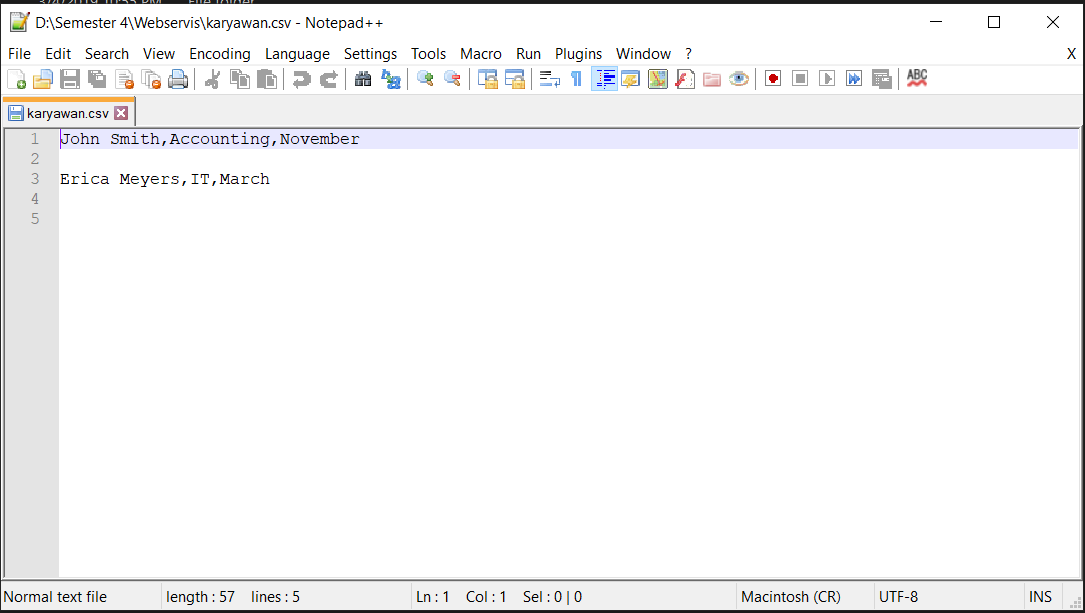
\includegraphics[width=0.5\textwidth]{figures/chapter4/1174040_csv.png}}
            \caption{Contoh CSV}
            \label{1174040_csv}
            \end{figure}

	\item Ms.Excel , NotePad, notepad++, sublime, dan texteditor lainnya

	\item caranya adalah :
		\begin{itemize}
			\item untuk write :
			\begin{enumerate}
				\item Download template csv
				\item Buka browser lalu menuju ke Google Sheet
				\item Tekan tombol merah di pojok kanan bawah
				\item Lalu pilih upload file untuk mengupload template yang sudah di download sebelumya
				\item Edit sesuai yang diinginkan
				\item Setelah selesai, lalukan eksport ke CSV dengan cara klik file lalu download as setelah itu pilih CSV
			\end{enumerate}
			\item untuk read :
			\begin{enumerate}
				\item buka Ms.Excel
				\item pilih Data lalu Get External Data dan pilih From Text
				\item lalu pilih file csv nya
				\item pilih Delimeted lalu Next
				\item checklist di box Tab dan Comma
				\item lalu klik finish
			\end{enumerate}
		\end{itemize}	
	\item Library CSV berisikan fungsi -fungsi dan kelas yang akan dipakai dalam pengerjaan file CSV

	\item Pandas diciptakan pada tahun 2008 oleh Wes McKinney dan diperbaharuin pada tahun 2010 oleh Sien Chang. yang fungsinya untuk melakukan analisa data seperti import dan export data.

	\item Fungsi - funsi library csv adalah :
		\begin{itemize}
			
			\item \begin{verbatim}csv.reader(csvfile, dialect='excel', **fmtparams)\end{verbatim} : digunakan untuk membaca line di csv
			\item \begin{verbatim}csv.writer(csvfile, dialect='excel', **fmtparams)\end{verbatim} : untuk menulis line di csv
			\item \begin{verbatim}csv.register_dialect(name[, dialect[, **fmtparams]]) \end{verbatim}: untuk asosiasikan dialect dengan name, dimana name harus string
			\item \begin{verbatim}csv.unregister_dialect(name)\end{verbatim} : menghapus dialect yang terasosiasi dengan name
			\item \begin{verbatim}csv.get_dialect(name)\end{verbatim} : mengnembalikan hasil dialect yang terasosisasi dengan name
			\item \begin{verbatim}csv.list_dialects() \end{verbatim}: menampilkan semua dialect yang ada
			\item \begin{verbatim}csv.field_size_limit([new_limit])\end{verbatim} : menamplikan field maksimal ayng di berikan oleh pembubat parse.

		\end{itemize}

	\item Pandas mengngunakan sistem dataframe yang memeprbolehkan kita untuk memasukkan sebuah file ke dalam tabel vitual seperti spreadsheet.kita dapat mengolah dengan fungsi - fungsi  seperti join, distinct, group by, agregasi dan funsi lain seperti dalam SQL tetapi dibuat pada tabel yang dimuat di file ke ram
	\end{enumerate}

\section{IrvanRizkiansyah/1174043}
	\subsection{Pemahaman Teori}
		\begin{enumerate}
			\item \begin{itemize}
					\item Fungsi : File csv berfungsi untuk pencarian data akan menjadi lebih mudah dan cepat, dan juga mempermudah penginputan data ke dalam database secara sederhana.
					\item Sejarah : File csv muncul pertama kali sekitar 10 tahun sebelum Personal Computer (PC) pertama  didunia yaitu sejak sekitar tahun 1972, akan tetapi sebutan file csv digunakan pertama kali pada tahun 1983.
					\item Contoh : 
						\begin{figure} [ht]
							\centerline{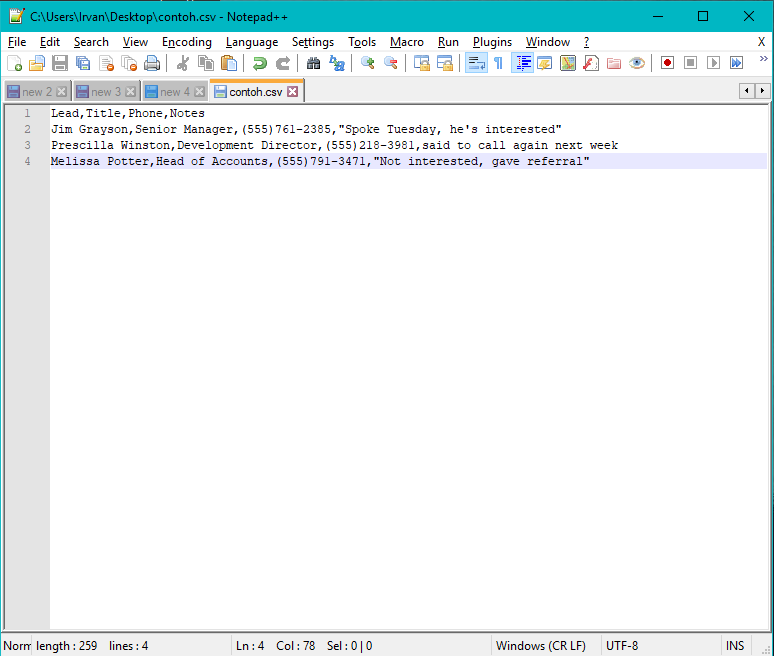
\includegraphics[width=0.6\textwidth]{figures/chapter4/Contoh_CSV.png}}
							\caption{Contoh CSV}
							\label{Contoh CSV}
						\end{figure}

					\ref{Contoh_CSV}
				\end{itemize}
			
			\item Ada banyak aplikasi yang dapat membuat file berformat CSV, diantaranya adalah :
				\begin{itemize}
					\item Notepad
					\item Notepad++
					\item Microsoft Excel
					\item Corel Quatro Pro
					\item Apache Open Office, dan masih banyak yang lainnya.
				\end{itemize}
			
			\item Cara menulis file csv menggunakan Excel :
				\begin{enumerate}
					\item Buka aplikasi Microsoft Excel kemudian buat dokumen baru
					\item Tulis judul kolom untuk setiap informasi yang ingin di rekam atau catat, kemudian tulis informasi - informasi dalam kolom dengan sesuai.
					\item Jika sudah selesai maka save dengan cara pilih menubar File lalu pilih Save As
					\item Lalu isikan nama file tersebut dan rubah dengan memilih format file yang tersedia tersebut menjadi .csv
					\item File csv sudah berhasil terbuat menggunakan Microsoft Excel
				\end{enumerate}
			\item Cara membaca file csv menggunakan Excel :
				\begin{enumerate}
					\item Buka aplikasi Microsoft Excel kemudian pilih menu Open
					\item Cari tempat file csv yang ingin dibuka, kemudian pilih Open
					\item File csv sudah berhasil dibaca menggunakan Microsoft Excel
				\end{enumerate}
			
			\item Pada file csv, tanda baca koma diartikan sebagai pembatas suatu kolom. List-directed input output didefinisikan dalam FORTRAN 77. List-directed input menggunakan tanda baca koma atau spasi sebagi pembatas, sehinnga karakter yang tidak dikutip tidak dapat mengandung tanda baca koma ataupun spasi. Hal tersebut yang diadopsi oleh file csv. format csv didukung dengan library untuk banyak bahasa pemrograman, kebanyakan yang menspesifikasikan pembatas field, pemisah desimal, pengkodean karakter, dan yang lainnya.
			
			\item Pada tahun 2008, pengembangan pandas dimulai oleh AQR Capital Management. Pada akhir tahun 2009 pandas menjadi Open Sourced, dimana disupport oleh banyak komunitas atau individu di dunia untuk mengembangkan pandas. Sejak tahun 2015, pandas menjadi NumFOCUS proyek sponsor, ini juga membantu suksesnya pengembangan dari pandas itu sendiri. pandas merupakan struktur data dan data analysis tools untuk bahasa pemrograman Python, dan merupakan BSD-licensed library yang menjadikannya memiliki performa yang tinggi.
			
			\item 
				\begin {itemize} 
					\item Tanda baca koma : Menjadi pemisah antar kolom
					\item Tanda baca kutip dua : Menjadi cara untuk memasukan sebuah kalimat atau untuk memasukan karakter spasi sebagai data pada kolom informasi
					\item Inputan pada baris pertama akan menjadi Header, dimana akan menjadi nama sebuah kolom, dan masih banyak yang lainnya
				\end{itemize}
			
			\item Pada pandas sedikit berbeda, dimana inputan data berbentuk seperti peng-inputan pada variabel pada umumnya, hanya saja menggunakan tanda kutip satu untuk menandakan sebuah informasi pada kolom kemudian tanda kurung kotak yang didalamnya berisi informasi data dari kolom tersebut. dan lain sebagainya.
			
		\end{enumerate}

\subsection{Luthfi Muhammad Nabil/1174035}
\subsubsection{Fungsi, Sejarah, dan Contoh file CSV}
\begin{itemize}
	\item Fungsi \linebreak File CSV (Comma Separated Values) adalah tipe file khusus yang menyimpan informasi dengan metode dipisahkan dengan koma. File CSV berfungsi untuk menjadi perantara untuk beberapa aplikasi yang memiliki basis data saat mengirim data. CSV dapat dibuka di berbagai text editor
	yang ada. Dengan bentuk filenya yang dinamis memungkinkan file CSV dapat dimanipulasi dan dapat menyimpan informasi dengan skala besar.
	\item Sejarah \linebreak CSV sudah digunakan sejak tahun 1972 yang dapat dikompilasi pada bahasa pemrograman IBM Fortran. Saat itu, data yang dipisahkan oleh koma jika isinya memiliki spasi maka harus diberi tanda petik di awal dan akhir isi dari data tersebut. Nama CSV baru mulai digunakan pada tahun 1983. Pada panduan dari Osborne Executive Computer mendokumentasikan kutipan yang membolehkan isi karakter memiliki koma.  Pada tahun 2005 dengan RFC4180, CSV didefinisikan sebagai MIME Content Type. lalu pada tahun 2013, defisiensi dari RFC4180 dipecahkan oleh rekomendasi dari W3C. Pada tahun 2014, IETF mempublikasi RFC7111 yang mendeskripsikan pecahan Uniform Resource Identifier(URI) ke dokumen CSV. RFC7111 menjelaskan bagaimana baris, kolom dapat dipilih dalam dokumen CSV menggunakan indeks posisi. Pada Tahun 2015, W3C mempublikasikan draft rekomendasi untuk CSV-metadata standards yang dimulai dengan rekomendasi pada bulan Desember dengan tahun yang sama. 
	\item Contoh File CSV \begin{itemize}
							\item 
							CSV pada Excel \ref{1174035_CSVExcel}
							\begin{figure}[!htbp]
								\centering
								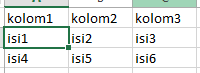
\includegraphics[height=4cm, width=7cm]{figures/chapter4/1174035_CSVExcel.jpg}
								\caption{Contoh CSV Pada Excel}
								\label{1174035_CSVExcel}
							\end{figure}
							\item \begin{figure}[!htbp]
								\centering
								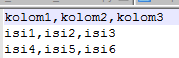
\includegraphics[height=4cm, width=7cm]{figures/chapter4/1174035_CSVText.jpg}
								\caption{Contoh CSV Pada Text}
								\label{1174035_CSVText}
							\end{figure}
							CSV pada Text Editor \ref{1174035_CSVText}
							
						  \end{itemize}
\end{itemize}
\subsubsection{Aplikasi Yang dapat membuat file CSV}
Berikut file yang dapat membuat file CSV
\begin{itemize}
	\item Spreadsheet \linebreak Spreadsheet merupakan aplikasi yang dapat membuat CSV hanya dengan memasukan data sesuai baris dan kolom yang diinginkan. Contoh spreadsheet seperti Google Spreadsheet, Microsoft Excel, dan aplikasi lainnya. 
	\item Bahasa Pemrograman \linebreak Bahasa pemrograman merupakan media yang dapat untuk membuat aplikasi yang dapat membuat file CSV khusus untuk bahasa pemrograman yang support dengan pembuatan file CSV. Seperti Python, C Sharp, dan lain sebagainya.
	\item Text Editor \linebreak Text editor juga dapat membuat file CSV, untuk membuat dengan Text Editor cukup dengan membuat file sesuai format CSV dan save file tersebut dengan ekstensi .CSV.
\end{itemize}
\subsubsection{Menulis dan Membaca file CSV}
Berikut cara menulis dan membaca file CSV : 
\begin{itemize}
	\item Menulis : \begin{enumerate}
						\item Buka file CSV dengan spreadsheet
						\item Klik Cell yang mau diisi
						\item Masukan data yang mau diisi pada cell tersebut
						\item Lalu save file dengan format .CSV
					\end{enumerate}
	\item Membaca : \begin{enumerate}
						\item Buka file CSV dengan spreadsheet						
					\end{enumerate}
\end{itemize}
\subsubsection{Sejarah Library CSV Python}
Library CSV pada python merupakan library yang paling umum untuk import export data pada spreadsheet dan basis data dengan format sesuai dengan standarisasi RFC4180. Seiring dengan lahirnya bahasa pemrograman python, library mulai dibuat dan dikembangkan sampai akhirnya pada tahun 2003, pembuatnya Kevin Altis dan lainnya telah merilis versi final untuk library Python CSV. 
\subsubsection{Sejarah Library Pandas Python}
Pandas (Python Data Analysis Library) adalah library open source yang digunakan untuk melakukan data manajemen dan data analysis. Pandas diciptakan pada tahun 2008 oleh Wes McKinney dan diperbaharui oleh Sien Chang pada tahun 2010. Inspirasi dari pembuatan pandas muncul pada komunitas yang membutuhkan library khusus untuk analisis data. 
\subsubsection{Fungsi - fungsi yang terdapat di library CSV}
\begin{itemize}
	\item \begin{verbatim} csv.reader(csvfile, dialect='excel', **fmtparams) \end{verbatim} Untuk mengembalikan	object reader yang akan mengambil setiap line pada csv yang diambil. Data setiap baris diambil saat next() dipanggil. Berikut contohnya : \lstinputlisting[firstline=1, lastline=6]{src/chapter4/chap4_1174035_teori.py}
	\item \begin{verbatim} csv.writer(csvfile, dialect='excel', **fmtparams) \end{verbatim} Mengembalikan file pembuat object untuk dapat mengkonversi data pada python ke file CSV yang akan dibuat. Berikut contoh penggunaan csv.writer : \lstinputlisting[firstline=8, lastline=14]{src/chapter4/chap4_1174035_teori.py}
	\item \begin{verbatim} csv.register_dialect(name[, dialect[, **fmtparams]]) \end{verbatim} Mengasosiasikan dialek dengan nama, nama yang dimasukkan harus berupa karakter.
	\item \begin{verbatim} csv.unregister_dialect(name) \end{verbatim}
	Menghapus asosiasi dialek dengan nama pada registry dialek.
	\item \begin{verbatim} csv.get_dialect(name) \end{verbatim}
	Mengambil dialek yang telah diasosiasikan dengan nama. 
	\item \begin{verbatim}  csv.list_dialects() \end{verbatim} Mengembalikan dialek yang telah diregistrasi.
	\item \begin{verbatim} csv.field_size_limit([new_limit]) \end{verbatim} Mengembalikan maksimal kolom data yang diperbolehkan oleh pembaca.
\end{itemize}
\subsubsection{Fungsi - fungsi yang terdapat di library Pandas}
\begin{itemize}
	\item \begin{verbatim} pandas.read_csv(filepath_or_buffer[, sep, …]) \end{verbatim} Untuk membaca file CSV dan menyimpannya ke DataFrame
	\item \begin{verbatim} pandas.read_excel(io[, sheet_name, header, names, …])  \end{verbatim} Membaca file excel dan menyimpannya ke DataFrame
	\item \begin{verbatim} to_csv([path, index, sep, na_rep, …]) \end{verbatim}
	Untuk membuat file CSV dari data yang ada	
\end{itemize}

\section{Faisal Najib Abdullah}
\subsection{Pemahaman Teori}
\begin{enumerate}
    \item Apa itu fungsi file csv, jelaskan sejarah dan contoh ?
    \par
    File CSV Nilai Berbatas Koma adalah tipe file khusus yang dapat Anda buat atau edit di Excel. File CSV menyimpan informasi yang dipisahkan oleh koma, bukan menyimpan informasi dalam kolom. Saat teks dan angka disimpan dalam file CSV, mudah untuk memindahkannya dari satu program ke program lain.
    \par 
	File CSV dibuat oleh program yang menangani sejumlah data yang besar. CSV merupakan cara yang nyaman untuk mengekspor data dari spreadsheet dan basis data serta mengimpor atau menggunakannya dalam program lain. Misalnya, Anda dapat mengekspor hasil program penambangan data ke file CSV dan kemudian mengimpornya ke dalam spreadsheet untuk menganalisis data, menghasilkan grafik untuk presentasi, atau menyiapkan laporan untuk publikasi.
    \par
	Contohnya, Anda dapat mengekspor kontak dari Google ke dalam file CSV, kemudian mengimpornya ke Outlook.
    
    \item Aplikasi-aplikasi apa saja yang bisa menciptakan file csv?
    Pada Windows
    \begin{itemize}
        \item Microsoft Excel 2013
        \item Microsoft Works
        \item CCorel Quattro Pro
        \item Apache OpenOffice
        \item LibreOffice
        \item Microsoft Notepad
        \item Intuit Quicken 2015
        \item GenScriber
    \end{itemize}
    Pada Mac OS
    \begin{itemize}
        \item Microsoft Excel 2011
        \item Planamesa NeoOffice
        \item Apache OpenOffice
        \item LibreOffice
        \item GenScriber
    \end{itemize}
    Pada Linux
    \begin{itemize}
        \item Apache OpenOffice
        \item LibreOffice
        \item GenScriber
    \end{itemize}
    
    \item Jelaskan bagaimana cara menulis dan membaca file csv di excel atau spreadsheet?
	\begin{itemize}
        \item Cara menulis file csv harus berupa baris dan kolom atau bisa juga di sebut berupa tabel.
        \item Untuk membacanya file csv dipisahkannya menggunakan koma atau titik koma.
    \end{itemize}
    
    \item Jelaskan sejarah library csv?
	Library csv menyediakan fungsionalitas untuk membaca dan menulis ke file CSV. Dirancang untuk bekerja di luar kotak dengan file CSV yang dihasilkan Excel, memudahkan untuk bekerja dengan berbagai format CSV. Library csv berisi objek dan kode lain untuk membaca, menulis, dan memproses data ke file CSV.
    
    \item Jelaskan sejarah library pandas?
	panda adalah pustaka Python open-source yang menyediakan alat analisis data kinerja tinggi dan struktur data yang mudah digunakan. panda tersedia untuk semua instalasi Python, tetapi itu adalah bagian penting dari distribusi Anaconda dan bekerja sangat baik di notebook Jupyter untuk berbagi data, kode, hasil analisis, visualisasi, dan teks naratif.

    \item Jelaskan fungsi-fungsi yang terdapat di library csv?
	Terdapat 2 fungsi yang bisa digunakan oleh library csv
    Pertama,fungsi membaca file csv.
    fungsi ini bisa menggunakan list dan dictionary
    Dengan list :
    \lstinputlisting[firstline=11, lastline=21]{src/chapter4/1174042_csv.py}
    Dengan dictionary :
    \lstinputlisting[firstline=24, lastline=33]{src/chapter4/1174042_csv.py}
    Kedua,fungsi menulis file csv.
    \lstinputlisting[firstline=36, lastline=40]{src/chapter4/1174042_csv.py}
    
    \item Jelaskan fungsi-fungsi yang terdapat di library pandas
	Hampir sama dengan library csv,tp library pandas penulisannya lebih sederhana dan terlihat lebih rapih dari pada library csv.
    \lstinputlisting[firstline=43, lastline=44]{src/chapter4/1174042_csv.py}
    

\end{enumerate}

\section{Fathi Rabbani / 1164074}
\subsection{Teori}
\begin{enumerate}
\item Sejarah dan Penjelasan CSV
\subitem Penggunaan dari format file CSV itu sendiri untuk memudahkan pembuatan data dengan menggunakan tanda koma sebagai pembatas dari datanya agar mudah untuk dibaca pada kolom.
\subitem CSV sendiri dibuat untuk dapat menangani pembuatan sejumlah data yang berukuran besar, mempermudah program dalam membaca datanya kedalam kolom - kolom. seperti contoh dalam membacanya menggunakan aplikasi Excel sehingga mempermudah dalam proses import dan eksport datanya. csv sendiri sudah ada pada tahun 1972 dengan pengembangnya adalah IBM namun penggunaannya masuk pada tahun 1983 yang berbarengan dengan adanya SuperCalc spreadsheet.

\item Aplikasi CSV
\begin{itemize}
\item Microsoft Excel
\item Open Office Calc
\item Google Docs
\item Libre Office
\item Apache Open Office
\end{itemize}

\item Menulis dan Membaca csv di Excel atau Spreadsheet
\subitem Menulis, cara menuliskan csv adalah dengan menggunakan tanda baca koma pada bagian data yang ingin dipisah contohnya \lstinputlisting[firstline=8, lastline=29]{src/chapter4/coba.csv}
\subitem Membaca, file csv dapat dibaca pada program aplikasi Excel dengan menampilkan hasil data dari setiap data yang dipisah dengan tanda baca koma menjadi kolom - kolom hasilnya ada pada \ref{fig1}

\item Library CSV
\subitem CSV atau comma separated value adalah salah satu tipe file yang digunakan secara luas di dunia programming. Tidak hanya itu CSV pun sering digunakan dalam pengolahan informasi yang dihasilkan spreadsheet untuk diproses lebih lanjut melalui mesin analitik. CSV pun dianggap sebagai file yang agnostik karena dapat digunakan oleh berbagai database untuk proses backup data.

\item Library Pandas
\subitem pandas merupakan library pada pemrograman python yang berguna untuk mengolah dan meyediakan struktur data serta analisa data yang mudah untuk dibaca dan dipahami seperti pada struktur data tabel. pandas dapat melakukan proses perbandingan data, penggabungan dataset, penanganan dataset yang hilang dll. pandas dapat juga digunakan sebagai pemrosesan data Statistik dengan pembacaan datanya menggunakan struktur Spreadsheet.

\item Fungsi pada Library CSV
\begin{itemize}
\item Menulis data CSV
\lstinputlisting[firstline=8, lastline=29]{src/chapter4/coba.csv}
\item Hasil dari menullis data CSV
\lstinputlisting[firstline=31, lastline=37]{src/chapter4/coba.csv}
\item Membaca data CSV
\lstinputlisting[firstline=40, lastline=52]{src/chapter4/coba.csv}
\item Hasil pembacaan data CSV
\lstinputlisting[firstline=54, lastline=60]{src/chapter4/coba.csv}
\end{itemize}

\item Fungsi pada Library Pandas
\begin{itemize}
\item Kode
\lstinputlisting[firstline=62, lastline=67]{src/chapter4/coba.csv}
\item Hasil
\lstinputlisting[firstline=69, lastline=73]{src/chapter4/coba.csv}
\end{itemize}
\end{enumerate}

\begin{figure}[!htbp]
	\centering
	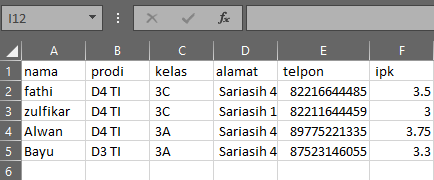
\includegraphics[width=1\textwidth]{figures/chapter4/1164074/1}
	\caption{hasil csv pada Excel}
	\label{fig1}
\end{figure}

\subsection{Praktek}
\begin{enumerate}
\item Fungsi Library CSV List
\lstinputlisting[firstline=1, lastline=8]{src/chapter4/1164074/c4_1164074_csv.py}
\item Fungsi Library CSV Dictionary
\lstinputlisting[firstline=10, lastline=16]{src/chapter4/1164074/c4_1164074_csv.py}
\item Fungsi Library pandas List
\lstinputlisting[firstline=1, lastline=4]{src/chapter4/1164074/c4_1164074_pandas.py}
\item Fungsi Library pandas Dictionary
\lstinputlisting[firstline=5, lastline=7]{src/chapter4/1164074/c4_1164074_pandas.py}
\item Fungsi Library pandas Date to DataFrame
\lstinputlisting[firstline=9, lastline=11]{src/chapter4/1164074/c4_1164074_pandas.py}
\item Fungsi Library pandas Index Colomn
\lstinputlisting[firstline=13, lastline=15]{src/chapter4/1164074/c4_1164074_pandas.py}
\item Fungsi Library pandas Change Att Colomn
\lstinputlisting[firstline=17, lastline=19]{src/chapter4/1164074/c4_1164074_pandas.py}
\item Fungsi Library CSV main.py
\lstinputlisting[firstline=1, lastline=7]{src/chapter4/1164074/main.py}
\item Fungsi Library pandas main2.py
\lstinputlisting[firstline=1, lastline=7]{src/chapter4/1164074/main2.py}
\end{enumerate}

\subsection{Error}
\begin{itemize}
\item Error Code
\subitem
ValueError: Date column tanggal already in dict
\item Keterangan Error
\subitem
data sudah berupa dictoinary sehingga tidak memerlukan pemecahan lagi dengan code berikut 
\lstinputlisting[firstline=5, lastline=6]{src/chapter4/1164074/1164074_Error.py}
\item Solusi
\subitem
\lstinputlisting[firstline=12, lastline=13]{src/chapter4/1164074/1164074_Error.py}
\end{itemize}

\section {Kevin Natanael Nainggolan 1174059}
	\begin {enumerate}
		\item Apa itu fungsi csv, jelaskan sejarah dan contohnya 
			\lstinputlisting [firstline=10, lastline=14]{src/teoric4.py}
		\item Aplikasi-aplikasi apa saja yang bisa menciptakan file csv? 
			\lstinputlisting [firstline=18, lastline=22]{src/teoric4.py}
		\item Jelaskan bagaimana cara menulis dan membaca file csv di excel atau spreadsheet
			\lstinputlisting [firstline=26, lastline=39]{src/teoric4.py}
		\item Jelaskan sejarah library csv
			\lstinputlisting [firstline=43, lastline=50]{src/teoric4.py}
		\item Jelaskan sejarah library pandas
			\lstinputlisting [firstline=54, lastline=60]{src/teoric4.py}
		\item Jelaskan fungsi-fungsi yang terdapat di library csv
			\lstinputlisting [firstline=64, lastline=68]{src/teoric4.py}
		\item Jelaskan fungsi-fungsi yang terdapat di library pandas
			\lstinputlisting [firstline=72, lastline=75]{src/teoric4.py}
	\end {enumerate}




\section{Yusniar Nur Syarif Sidiq/1164089}
\subsection{Pemahaman Teori}

\begin{enumerate}

\item Apa itu fungsi file csv, jelaskan sejarah dan contoh.
	\subitem File csv merupakan jenis file khusus yang dapat kita buat dan edit di dalam Excel. File csv akan menyimpan informasi data yang dipisahkan dengan koma atau tanda titik koma, dimana artinya file csv tidak menyimpan data dalam bentuk kolom. Saat pertama kali rilis, excel menggunakan format file dalam bentuk biner yaitu BIFF sebagai format file utama. Namun setelah Microsoft merilis Ofice System 2007, Excel telah menggantikan format utamanya menjadi XML. Meskipun mendukung format XML baru, Excel masih mendukung format BIFF, tidak hanya itu excel juga telah mendukung format CSV, DBF, SYLK, DIF, dan format-format lainnya. Fungsi dari file csv itu sendiri adalah mempermudah dalam pencarian data dan pengimputan data ke dalam database sederhana. File csv mulai digunakan pada tahun 1983 akan tetapi format file csv sudah ada dari tahun 1972. Contoh file dengan format csv dapat dilihat pada figure \ref{YNCSV1}

	\begin{figure}[ht]
		\centering{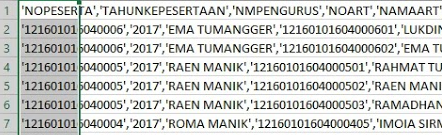
\includegraphics[scale=0.5]{figures/chapter4/YN/Chapter4/YNCSV1.png}}
		\caption{Contoh File CSV}
		\label{YNCSV1}
	\end{figure}

\item Aplikasi - aplikasi apa saja yang bisa menciptakan file csv.
	\subitem Untuk membuat file dengan format CSV, kita dapat menggunakan software bawaan Microfsoft Ofice yaitu Excel. Bukan hanya Microsoft Excel, kita juga dapat membuat file CSV dengan bantuan text editor. Jika kita ingin membuat file csv secara online dapat menggunakan Google Spreadshare. Apabila OS PC kita menggunakan Linux dapat menggunakan LibreOfficecalc.

\item Jelaskan bagaimana cara menulis dan membaca file csv di excel atau spreadsheet.
	\subitem Cara membuat file CSV dengan Excel
			\begin{itemize}
				\item Buka software Microsoft Excel
				\item Pilih new document
				\item Buatlah judul kolom yang ingin kita rekam
				\item Isikan informasi - informasi pada setiap kolom
				\item Simpan dengan menggunakan metode save as
				\item Cari dan pilih format csv
				\item Pilih button save untuk melakukan penyimpanan
			\end{itemize}
	\subitem Cara membaca file CSV dengan Excel
			\begin{itemize}
				\item Buka software Microsoft Excel
				\item Lakukan perintah open file
				\item Cari file csv yang sudah kita buat sebelumnya
				\item Pilih button open untuk membaca file csv pada Microsoft Excel
			\end{itemize}
	\subitem Cara membaca file csv dari Excel
		\lstinputlisting[firstline=1, lastline=9]{src/chapter4/1164089.py}
	\subitem Cara membuat file csv
		\lstinputlisting[firstline=12, lastline=16]{src/chapter4/1164089.py}

\item Jelaskan sejarah library csv. 
	\subitem Pada tahun 1972 adalah terbentuknya format file csv namun bukan hanya itu saja, pada saat itupun terbentuk juga yang namanya library pandas.Seiring dengan lahirnya bahasa pemrograman python, library mulai dibuat dan dikembangkan oleh Kevin Altis. Dengan kata lain CSV dibentuk pada tahun 1972 dan sudah satu paket baik dalam librarynya maupun format filenya. 

\item Jelaskan sejarah library pandas.
	\subitem Developer yang bernama Wes McKinney telah mengajarkan pandas pada tahun 2008 ketika ia berada di AQR Capital Management, karena kebutuhan akan alat kinerja tinggi yang fleksibel untuk melakukan analisis kuantitatif pada data keuangan. Sebelum meninggalkan AQR, dia dapat meyakinkan manajemen untuk mengizinkan membuka sumber library. Pegawai AQR lainnya yaitu Chang She, telah bergabung dengan upaya ini pada 2012 sebagai kontributor utama kedua ke library. Pada tahun 2015, pandas telah menandatangani sebagai proyek NumFocus yang disponsori secara fiskal. Pada saat itulah Library Pandas mulai berjalan dan digunakan.

\item Jelaskan fungsi-fungsi yang terdapat di library csv.
	\subitem Ada dua fungsi pada library csv, yaitu csv.reade dan csv.writer. Dimana fungsi tersebut memiliki tugas yang berbeda-beda. Untuk csv.reader bertugas sebagai membaca file csv sedangkan csv.writer bertugas membuat file csv.

\item Jelaskan fungsi-fungsi yang terdapat di library pandas.
	\subitem Untuk library pandas sama saja dengan library csv namun bedanya hanya cara penulisan source codenya saja. Untuk membaca file csv pada library pandas membutuhkan perintah pandas.read\_csv sedangkan untuk membuat file csv membutuhkan perintah pandas.write\_csv.

\end{enumerate}

\subsection{Keterampilan Pemrograman}
\begin{enumerate}
	\item Membaca file csv pada lib csv dengan mode list

		\lstinputlisting[firstline=1, lastline=9]{src/chapter4/1164089/1164089_csv.py}

	\item Membaca file csv pada lib csv dengan mode dictionary

		\lstinputlisting[firstline=11, lastline=16]{src/chapter4/1164089/1164089_csv.py}

	\item Membaca file csv pada lib pandas dengan mode list
		
		\lstinputlisting[firstline=1, lastline=7]{src/chapter4/1164089/1164089_pandas.py}

	\item Membaca file csv pada lib pandas dengan mode dictionary

		\lstinputlisting[firstline=9, lastline=13]{src/chapter4/1164089/1164089_pandas.py}

	\item Mengubah format tanggal menjadi standar DataFrame

		\lstinputlisting[firstline=15, lastline=18	]{src/chapter4/1164089/1164089_pandas.py}
	
	\item Mengubah index kolom

		\lstinputlisting[firstline=21, lastline=25]{src/chapter4/1164089/1164089_pandas.py}

	\item Mengubah atribut atau nama kolom

		\lstinputlisting[firstline=26, lastline=30]{src/chapter4/1164089/1164089_pandas.py}

	\item Membuat program NPM\_main.py dan isikan bagaimana cara membaca file csv dan membuat file csv

		\lstinputlisting[firstline=1, lastline=6]{src/chapter4/1164089/1164089_main.py}
	
	\item Membuat program NPM\_main2.py dan isikan bagaimana cara membaca file csv dan membuat file csv dengan lib pandas

		\lstinputlisting[firstline=1, lastline=6]{src/chapter4/1164089/1164089_main2.py}
	

\end{enumerate}

\subsection{Penaganan Error}

\begin{enumerate}

	\item Tuiskan peringatan error yang di dapat dari mengerjakan praktek ketiga ini, dan jelaskan cara penanganan error tersebut. Buatlah fungsi try except untuk mengulangi error tersebut.

	\subitem Dimana error yang saya dapat merupakan atribute error yaitu dimana kondisi penulisan source code atribute salah atau tidak ditemukan, untuk lebih jelasnya dapat dilihat pada figure \ref{YNC4-3}

	\begin{figure}[ht]
		\centering{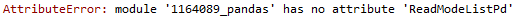
\includegraphics[scale=0.5]{figures/chapter4/YN/Chapter4/YNC4-3.png}}
		\caption{Atribute Error}
		\label{YNC4-3}
	\end{figure}

Cara penganannya yaitu ubah atribute yang terdapat pada file python sama dengan yang kita buat di file sebelumnya. Coontohnya dapat dilihat pada figure \ref{YNC4-4}

	\begin{figure}[ht]
		\centering{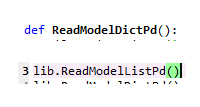
\includegraphics[scale=0.5]{figures/chapter4/YN/Chapter4/YNC4-4.png}}
		\caption{Atribute Error}
		\label{YNC4-4}
	\end{figure}

Dimana penulisannya harus sama persis dikarenakan Python bersifat case sensitif.

	\subitem Untuk penulisan Try Ecept dapat dilihat pada source code dibawah ini,

	\lstinputlisting[firstline=42, lastline=47]{src/chapter4/1164089/1164089_pandas.py}


\end{enumerate}

\section{Alit Fajar Kurniawan  1174057}
	\subsection{Pemahaman Teori}
		\begin{enumerate}
			\item 
			\begin{itemize}
					\item Fungsi : File csv berfungsi melakukan pencarian data agar menjadi lebih mudah dan cepat, dan juga mempermudah penginputan 
					data ke dalam database secara lebih sederhana.
					\item Sejarah : Pada 10 tahun yang lalu File csv muncul pertama kali sebelum Personal Computer pertama  di dunia sejak 
					sekitar tahun 1972, akan tetapi sebutan file csv digunakan pertama kali pada tahun 1983.
					\item Contohnya : Anda dapat mengekspor kontak dari Google ke dalam file CSV, kemudian mengimpornya ke Outlook.
			\end{itemize}
			
			\item Ada banyak aplikasi yang dapat membuat file berformat CSV, diantaranya adalah :
				    Pada Windows
					\begin{itemize}
						\item Microsoft Excel 2013
						\item Microsoft Works
						\item CCorel Quattro Pro
						\item Apache OpenOffice
						\item LibreOffice
						\item Microsoft Notepad
						\item Intuit Quicken 2015
						\item GenScriber
					\end{itemize}
					Pada Linux
					\begin{itemize}
						\item Apache OpenOffice
						\item LibreOffice
						\item GenScriber
					\end{itemize}
					Pada Mac OS
					\begin{itemize}
						\item Microsoft Excel 2011
						\item Planamesa NeoOffice
						\item Apache OpenOffice
						\item LibreOffice
						\item GenScriber
					\end{itemize}
					
			\item Jelaskan bagaimana cara menulis dan membaca file csv di excel atau spreadsheet?
				\begin{itemize}
					\item Untuk menulis file csv harus berupa baris dan kolom atau bisa juga di sebut berupa tabel.
					\item Untuk membacanya file csv dipisahkannya menggunakan koma atau titik koma.
			\end{itemize}
			
			\item sejarah library csv : Library csv menyediakan fungsionalitas untuk membaca dan menulis ke file CSV. Dirancang untuk bekerja di luar kotak dengan file CSV 
			yang dihasilkan Excel, memudahkan untuk bekerja dengan berbagai format CSV. Library csv berisi objek dan kode lain untuk membaca, menulis, 
			dan memproses data ke file CSV.
			
			\item Sejarah library pandas : Tahun 2008, pengembangan pandas dimulai oleh AQR Capital Management. Pada akhir tahun 2009 pandas menjadi Open Sourced, 
			dimana disupport oleh banyak komunitas atau individu di dunia untuk mengembangkan pandas. Sejak tahun 2015, 
			pandas menjadi NumFOCUS proyek sponsor, ini juga membantu suksesnya pengembangan dari pandas itu sendiri. 
			pandas merupakan struktur data dan data analysis tools untuk bahasa pemrograman Python, 
			dan merupakan BSD-licensed library yang menjadikannya memiliki performa yang tinggi.
			
			\item Jelaskan fungsi-fungsi yang terdapat di library csv?
			Terdapat 2 fungsi yang bisa digunakan oleh library csv
			Pertama,fungsi membaca file csv.
			fungsi ini bisa menggunakan list dan dictionary
			Dengan list :
			\lstinputlisting[firstline=11, lastline=21]{src/chapter4/1174057csvpandas.py}
			Dengan dictionary :
			\lstinputlisting[firstline=24, lastline=33]{src/chapter4/1174057csvpandas.py}
			Kedua,fungsi menulis file csv.
			\lstinputlisting[firstline=36, lastline=40]{src/chapter4/1174057csvpandas.py}
			
			\item Jelaskan fungsi-fungsi yang terdapat di library pandas
			Hampir sama dengan library csv,tp library pandas penulisannya lebih sederhana dan terlihat lebih rapih dari pada library csv.
			\lstinputlisting[firstline=43, lastline=44]{src/chapter4/1174057csvpandas.py}
    
		\end{enumerate}
		
	\subsection{Keterampilan Pemograman}
		\begin{enumerate}
			\item Buatlah  fungsi  (file  terpisah/library  dengan  nama  NPMcsv.py)  untuk  membuka file csv dengan lib csv mode list.
			\lstinputlisting[caption = Fungsi untuk membuka file CSV dengan lib CSV mode list., firstline=10, lastline=15]{src/Chapter4/1174057/1174057csv.py}
	
			\item Buatlah  fungsi  (file  terpisah/library  dengan  nama  NPMcsv.py)  untuk  membuka file csv dengan lib csv mode dictionary.
			\lstinputlisting[caption =  Fungsi untuk membuka file CSV dengan lib CSV mode dictionary., firstline=17, lastline=22]{src/Chapter4/1174057/1174057csv.py}
			
			\item Buatlah fungsi (file terpisah/library dengan nama NPMpandas.py) untuk membuka file csv dengan lib pandas mode list.	
			\lstinputlisting[caption =  Fungsi untuk membuka file CSV dengan lib Pandas mode list., firstline=10, lastline=13]{src/Chapter4/1174057/1174057pandas.py}
			
			\item Buatlah fungsi (file terpisah/library dengan nama NPMpandas.py) untuk membuka file csv dengan lib pandas mode dictionary.			
			\lstinputlisting[caption =  Fungsi untuk membuka file CSV dengan lib Pandas mode dictionary., firstline=15, lastline=19]{src/Chapter4/1174057/1174057pandas.py}
			
			\item  Buat fungsi baru di NPMpandas.py untuk mengubah format tanggal menjadi standar dataframe.			
			\lstinputlisting[caption =  Fungsi untuk mengubah format tanggal menjadi standar dataframe., firstline=21, lastline=24]{src/Chapter4/1174057/1174057pandas.py}
			
			\item Buat fungsi baru di NPMpandas.py untuk mengubah index kolom.			
			\lstinputlisting[caption =  Fungsi untuk mengubah index kolom., firstline=26, lastline=30]{src/Chapter4/1174057/1174057pandas.py}
			
			\item Buat fungsi baru di NPMpandas.py untuk mengubah atribut atau nama kolom.			
			\lstinputlisting[caption =  Fungsi untuk mengubah atribut atau nama kolom., firstline=32, lastline=36]{src/Chapter4/1174057/1174057pandas.py}
			
			\item Buat program main.py yang menggunakan library NPMcsv.py yang membuat dan membaca file csv.			
			\lstinputlisting[caption =  Membuat dan mebaca file CSV menggunakan library 1174006pandas., firstline=8, lastline=13]{src/Chapter4/1174057/main.py}
			
			\item Buat program main2.py yang menggunakan library NPMpandas.py yang membuat dan membaca file csv.			
			\lstinputlisting[caption = Membuat dan mmebaca file CSV menggunakan library 1174006pandas., firstline=8, lastline=13]{src/Chapter4/1174057/main2.py}
			
		\end{enumerate}
	
	\subsection{Ketrampilan Penanganan Error}
			Error yang di dapatkan dari mengerjakan tugas ini adalah type error, mengatasinya dengan cara mengecheck kembali codingannya
			kemudian run kembali aplikasinya
			berikut contoh Penggunaan fungsi try dan exception

			\lstinputlisting{src/chapter4/1174057/1174057_error.py}
\section {Kevin Natanael Nainggolan 1174059}
	\begin{enumerate}
		\item Apa itu fungsi csv, jelaskan sejarah dan contohnya 
			\lstinputlisting [firstline=10, lastline=14]{src/teoric4.py}
		\item Aplikasi-aplikasi apa saja yang bisa menciptakan file csv? 
			\lstinputlisting [firstline=18, lastline=22]{src/teoric4.py}
		\item Jelaskan bagaimana cara menulis dan membaca file csv di excel atau spreadsheet
			\lstinputlisting [firstline=26, lastline=39]{src/teoric4.py}
		\item Jelaskan sejarah library csv
			\lstinputlisting [firstline=43, lastline=50]{src/teoric4.py}
		\item Jelaskan sejarah library pandas
			\lstinputlisting [firstline=54, lastline=60]{src/teoric4.py}
		\item Jelaskan fungsi-fungsi yang terdapat di library csv
			\lstinputlisting [firstline=64, lastline=68]{src/teoric4.py}
		\item Jelaskan fungsi-fungsi yang terdapat di library pandas
			\lstinputlisting [firstline=72, lastline=75]{src/teoric4.py}
	\end {enumerate}	
	\begin{enumerate}
			\item\lstinputlisting{src/chapter4/1174057/1174057_error.py}	
	\end{enumerate}
			
\section{Muhammad Iqbal Panggabean 1174063}
\subsection{Praktek}
\begin{enumerate}
	\item Buatlah  fungsi  (file  terpisah/library  dengan  nama  NPMcsv.py)  untuk  membuka file csv dengan lib csv mode list.
	
	\lstinputlisting[caption = Fungsi untuk membuka file CSV dengan lib CSV mode list., firstline=10, lastline=15]{src/chapter4/1174063/1174063csv.py}
	
	\item Buatlah  fungsi  (file  terpisah/library  dengan  nama  NPMcsv.py)  untuk  membuka file csv dengan lib csv mode dictionary.
	
	\lstinputlisting[caption =  Fungsi untuk membuka file CSV dengan lib CSV mode dictionary., firstline=17, lastline=22]{src/chapter4/1174063/1174063csv.py}
	
	\item Buatlah fungsi (file terpisah/library dengan nama NPMpandas.py) untuk membuka file csv dengan lib pandas mode list.
	
	\lstinputlisting[caption =  Fungsi untuk membuka file CSV dengan lib Pandas mode list., firstline=10, lastline=13]{src/chapter4/1174063/1174063pandas.py}
	
	\item Buatlah fungsi (file terpisah/library dengan nama NPMpandas.py) untuk membuka file csv dengan lib pandas mode dictionary.
	
	\lstinputlisting[caption =  Fungsi untuk membuka file CSV dengan lib Pandas mode dictionary., firstline=10, lastline=13]{src/chapter4/1174063/1174063pandas.py}
	
	\item  Buat fungsi baru di NPMpandas.py untuk mengubah format tanggal menjadi standar dataframe.
	
	\lstinputlisting[caption =  Fungsi untuk mengubah format tanggal menjadi standar dataframe., firstline=15, lastline=19]{src/chapter4/1174063/1174063pandas.py}
	
	\item Buat fungsi baru di NPMpandas.py untuk mengubah index kolom.
	
	\lstinputlisting[caption =  Fungsi untuk mengubah index kolom., firstline=21, lastline=24]{src/chapter4/1174063/1174063pandas.py}
	
	\item Buat fungsi baru di NPMpandas.py untuk mengubah atribut atau nama kolom.
	
	\lstinputlisting[caption =  Fungsi untuk mengubah atribut atau nama kolom., firstline=26, lastline=30]{src/chapter4/1174063/1174063pandas.py}
	
	\item Buat program main.py yang menggunakan library NPMcsv.py yang membuat dan membaca file csv.
	
	\lstinputlisting[caption =  Membuat dan mebaca file CSV menggunakan library 1174006pandas., firstline=8, lastline=13]{src/chapter4/1174063/1174063main.py}
	
	\item Buat program main2.py yang menggunakan library NPMpandas.py yang membuat dan membaca file csv.
	
	\lstinputlisting[caption = Membuat dan mmebaca file CSV menggunakan library 1174006pandas., firstline=8, lastline=13]{src/chapter4/1174063/1174063main2.py}
\end{enumerate}

\subsection{Ketrampilan Penanganan Error}
Error yang di dapat dari mengerjakan tugas ini adalah type error, cara menaggulaginya dengan cara mengecheck kembali codingannya
kemudian run kembali aplikasinya
berikut contoh Penggunaan fungsi try dan exception
\lstinputlisting{src/chapter4/1174063/1174063_2err.py}



\chapter{Judul Bagian Kelima}
\section{Alit Fajar Kurniawan}
{\Large \textbf{Pemahaman Teori}}
\subsection{No. 1}
Apa itu fungsi device manager di windows dan folder /dev di linux?

	\hfill \break
	Device manager adalah perangkat lunak untuk menampilkan seluruh perangkat keras yang diinisialisasi atau sudah terhubung dengan sistem operasi Windows. Perangkat keras tersebut bisa berupa harddisk, kartu VGA, sound, keyboard, perangkat USB dan lain-lainnya. fungsi lain dari device manager yaitu, Menunjukkan status mengenai suatu perangkat keras,
	Mengelola driver perangkat keras, Menonaktifkan dan mengaktifkan perangkat keras, Menunjukkan informasi detail mengenai suatu perangkat keras, Mengidentifikasi konflik antar perangkat keras, dan Memberitahukan terjadinya masalah pada perangkat keras.

	\hfill \break
	Folder /dev merupakan representasi dari drive yang terhubung ke sistem operasi Linux dan oleh sistem dianggap sebagai file-file direktori. Biasanya sering ditampilkan direktori seperti /dev/sda1 yang mewakili Drive SATA pertama dalam sistem.

\subsection{No. 2}
Jelaskan langkah-langkah instalasi driver dari arduino!

	\hfill \break
	Berikut ini adalah langkah-langkah instalasi driver dari Arduino UNO di Windows:

	\begin{enumerate}
		\item Pertama pastikan Arduino IDE telah terinstall.
		\item Lalu hubungkan port USB Arduino Uno ke port USB PC.
		\item Kemudian PC anda akan mendeteksi perangkat baru yang terpasang dan akan muncul pop seperti ini.
		\item Karena Arduino Uno baru pertama kali terpasang, maka akan muncul pop up error seperti ini.
		\item Buka ''Start'' lalu cari Device Manager, kemudian klik ''Device Manager''.
		\item Setelah Device Manager terbuka, silahkan cari ''Unknown Device'' yang berada di Other Device.
		\item Kemudian klik kanan pada ''Unknown Device'', lalu pilih ''Update Driver Software''.
		\item Setelah itu muncul window baru, lalu pilih ''Browse my computer for driver software''.
		\item Lalu cari folder yang terinstall Arduino IDE dengan mengklik browse. Kemudian klik ''Next''.
		\item Windows akan mencari dan menginstall driver yang berada pada folder tersebut.
		\item Setelah itu akan muncul window, lalu klik ''Install''.
		\item Jika berhasil terinstal maka akan muncul window seperti ini.
	\end{enumerate}

\subsection{No. 3}
	\begin{itemize}
		\item Membaca Baudrate dari Komputer
			\begin{enumerate}
				\item Pertama buka ''Start''. Cari ''Device Manager'', lalu klik.
				\item Kemudian pilih ''Ports (COM \& LPT)''.
				\item Klik dua kali pada COM yang terhubung.
				\item Pilih tab ''Port Settings'', lalu lihat di ''Bit per second''.
			\end{enumerate}
		\item Membaca Port dari Komputer
			\begin{enumerate}
				\item Pertama buka ''Start''. Cari ''Device Manager'', lalu klik.
				\item Kemudian pilih ''Ports (COM \& LPT)''.
				\item Port dari Arduino telah terbaca oleh PC.
			\end{enumerate}
	\end{itemize}
	
\subsection{No. 4}
	Jelaskan sejarah library pyserial!

	\hfill \break
	PySerial adalah paket Python yang menfasilitasi komunikasi serial antara PC dengan perangkat keras eksternal. PySerial menyediakan antarmuka untuk berkomunikasi melalui protokol komunikasi serial. Komunikasi serial adalah salah satu protokol komunikasi komputer tertua. Protokol komunikasi serial mendahului spesifikasi USB yang digunakan oleh komputer dan perangkat keras lain seperti mouse, keyboard, dan webcam. USB adalah singkatan dari Universal Serial Bus. USB dan dibangun di atas dan memperluas antarmuka komunikasi serial asli.

\subsection{No. 5}
	Jelaskan fungsi-fungsi apa saja yang dipakai dari library pyserial!

	\hfill \break
	Fungsi-fungsi yang dipakai dari library PySerial, yaitu:
	\begin{enumerate}
		\item Serial - fungsi ini untuk membuka port serial.
		\item write(data) - fungsi ini menulis data lewat port serial.
		\item readline - fungsi ini membaca sebuah string dari port serial.
		\item read(size) - fungsi ini untuk membaca jumlah byte dari port serial.
		\item close - fungsi ini untuk menutup port serial.
	\end{enumerate}

\subsection{No. 6}
	Jelaskan kenapa butuh perulangan dan tidak butuh perulangan dalam membaca serial!

	\hfill \break
	Pada saat membaca serial di Arduino diperlukan perulangan agar bisa membaca data secara berulang kali sehingga data yang muncul banyak. Sedangkan apabila tidak membutuhkan perulangan maka Arduino hanya akan membaca data sekali saja.

\subsection{No. 7}
	Jelaskan bagaimana cara membuat fungsi yang mengunakan pyserial!

	\lstinputlisting[caption = Fungsi yang menggunakan pyserial., firstline=1, lastline=13]{src/chapter5/teori/1174057.py}

	\subsection{Cek Plagiat}
	\begin{figure}[H]
		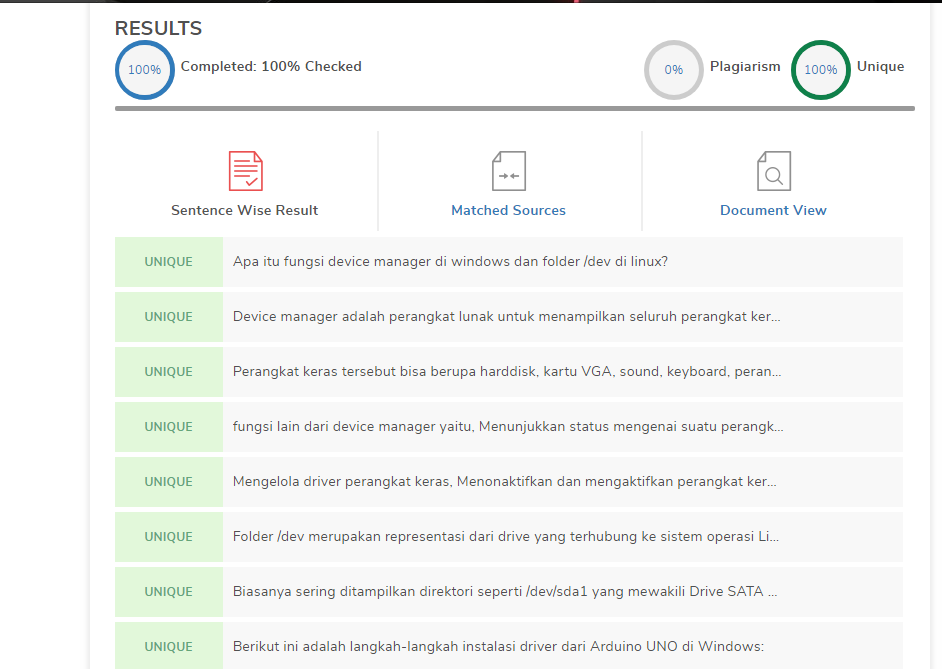
\includegraphics[width=10cm]{figures/chapter5/1174057/teori/plagiarisme.png}
		\centering
		\caption{Hasil cek plagiat}
	\end{figure}
	
	
\section{Muhammad Iqbal Panggabean}
{\Large \textbf{Pemahaman Teori}}
\subsection{Pertanyaan No.. 1}
Apa itu fungsi device manager di windows dan folder /dev di linux?

\hfill \break
Fungsi device manager antara lain :
\begin{enumerate}
	\item Mengidentifikasi konflik antar perangkat keras.
	\item Menunjukkan informasi detil suatu hardware.
	\item Disable dan Enable hardware.
	\item Mengelola driver hardware.
	\item Menunjukkan status suatu hardware.
\end{enumerate}

\hfill \break
Folder /dev berisi file device, baik device blok maupun device karakter. Di dalamnya setodaknya ada file biner yang beernama MAKEDEV untuk membuat device secara manual.

\subsection{Pertanyaan No. 2}
Jelaskan langkah-langkah instalasi driver dari arduino!

\hfill \break
Berikut ini adalah langkah-langkah instalasi driver dari Arduino UNO di Windows:

\begin{enumerate}
	\item Hubungkan sistem minimun Arduino Uno ke komputer dengan kabel USB type B (kabel Printer).
	\item Lalu pada bagian kanan didesktop PC anda, akan muncul popup “Installing device driver software”.
	\item SIstem operasi Windows tidak menyediakan driver untuk Arduino Uno.
	\item Buka Device Manager, caranya pada bagian Search Program and Files lalu ketikkan “device manager” (tanpa tanda petik). Kemudian bagian Control Panel akan muncul halaman Device Manager, selanjutnya klik untuk menjalankan.
	\item Cari yang bernama Unknown device yang berada pada bagian Other device, biasanya ada tanda seru berwarna kuning, itu disebabkan karena penginstallan tidak berjalan dengan sempurna.
	\item Klik kanan pada “Unknown device” kemudian pilih Update Driver Software.
	\item Pilih Browse my computer for driver software.
	\item Arahkan lokasi folder ke folder ..arduino-1.0.5 drivers. Pastikan check-box lalu centang include subfolders. Klik Next untuk melanjutkan instalasi driver.
	\item Kemudian lanjutkan dengan mengklik Install pada tampilan Windows Security.
	\item Jika instalasi driver berhasil maka akan muncul Windows has successfully updated your driver software.
	\item Perhatikan dan ingat nama COM Arduino Uno, karena nama COM ini yang akan digunakan untuk meng-upload program nantinya.
\end{enumerate}

\subsection{Pertanyaan No. 3}
Jelaskan bagaimana cara membaca baudrate dan port dari komputer yang sudah terinstall driver!

\hfill \break
\textbf{Membaca Port dari Komputer}

\begin{enumerate}
	\item Hubungkan modul TX-RX serial dengan komputer melalui serial port menggunakan DB9 cable extension.
	\item Buka Hyper Terminal dengan menekan start kemudian All progams lalu Accessories kemudian Communications lalu Hyper Terminal.
	\item Ketik nama untuk Connection Description, misal coba, kemudian tekan OK.
	\item Pada Connect to, pilihlah COM port yang dipakai di Connect using, kemudian tekan OK.
	\item Masukkan nilai-nilai port settingnya, sesuai dengan DCE-nya. Kemudian tekan OK.
\end{enumerate}



\subsection{Pertanyaan No. 4}
Jelaskan sejarah library pyserial!

\hfill \break
PySerial adalah library/modul Python siap-pakai dan gratis yang dibuat untuk memudahkan kita dalam membuat program komunikasi data serial RS232 dalam bahasa Python.
Jika modul USB-2REL dapat kita kontrol dengan mudah menggunakan Python dan PyUSB (lihat pembahasannya di sini dan di sini), maka modul SER-2REL juga dapat kita kontrol dengan mudah menggunakan Python dengan bantuan modul PySerial.

\subsection{Pertanyaan No. 5}
Jelaskan fungsi-fungsi apa saja yang dipakai dari library pyserial!

\hfill \break
Fungsi-fungsi yang dipakai dari library PySerial, yaitu:
\begin{enumerate}
	\item Serial - fungsi ini untuk membuka port serial.
	\item write(data) - fungsi ini menulis data lewat port 
	\item serial.close() - fungsi ini untuk menutup port serial.
	\item readline() - fungsi ini membaca sebuah string dari port serial.
	\item read(size) - fungsi ini untuk membaca jumlah byte dari port serial.
\end{enumerate}

\subsection{Pertanyaan No. 6}
Jelaskan kenapa butuh perulangan dan tidak butuh perulangan dalam membaca serial!

\hfill \break
Pada saat membaca serial di Arduino diperlukan perulangan agar bisa membaca data secara berulang kali sehingga data yang muncul banyak. Sedangkan apabila tidak membutuhkan perulangan maka Arduino hanya akan membaca data sekali saja.

\subsection{Pertanyaan No. 7}
Jelaskan bagaimana cara membuat fungsi yang mengunakan pyserial!

\hfill \break
Fungsi yang berada pada Python, dibuat dengan nama kata kunci def kemudian diikuti dengan nama fungsinya pada pyhton.
Seperti halnya dengan blok kode yang lain, kita juga harus memberikan identasi untuk menuliskan isi fungsi.

\subsection{Cek Plagiat}
\begin{figure}[H]
	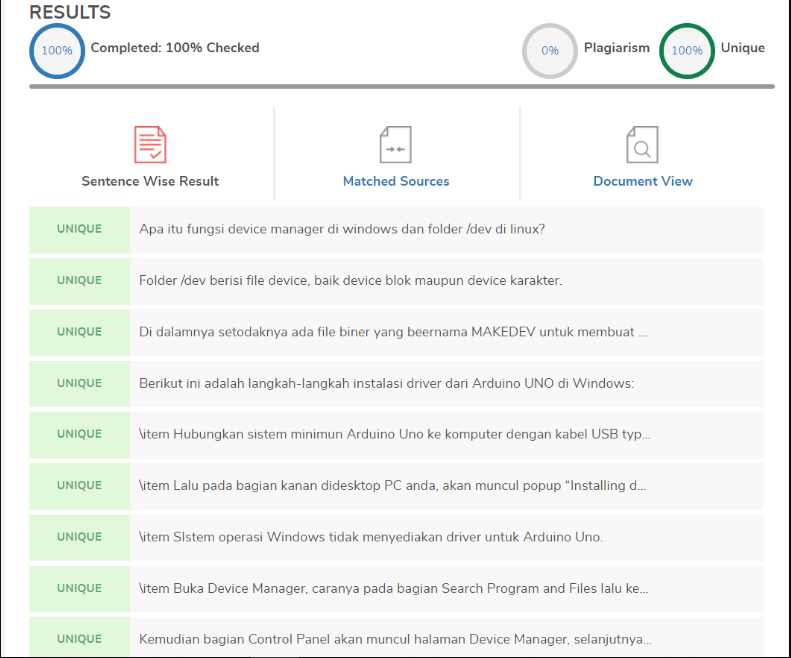
\includegraphics[width=10cm]{figures/chapter5/1174063/plagiatgabe}
	\centering
	\caption{Hasil cek plagiat.}
\end{figure}

\section{Fathi Rabbani / 1164074}
\subsection{Teori}
\begin{enumerate}
\item Fungsi Device manager pada Windows dan folder /dev pada Linux
\subitem Device Manager dalam komputer Windows merupakan perluasan dari Microsoft Management Console. Device Manager menampilkan seluruh hardware yang bisa di-inisialisasi (dikenali) oleh Windows. Tampilannya sudah ter-organisir (dikelompokkan) sedemikian rupa sehingga akan memudahkan pengelolaan setiap hardware yang ada. berikut ini adalah kegunaan dari Device Manager :
\begin{itemize}
\item Menunjukkan status suatu hardware
\item Menunjukkan informasi detil suatu hardware
\item Mengelola driver hardware
\item Disable dan Enable hardware
\item Meng-identifikasi konflik antar hardware, dll.
\end{itemize}

\subitem folder /dev pada linux merupakan direktori yang berfungsi untuk menyimpan konfigurasi device atau hardware dari sistem, seperti harddisk (hda, sda), terminal (tty) etc.

\item Instalasi Driver Arduino
\subitem Berikut ini adalah tahapan dalam melakukan proses instalasi Driver Arduino pada OS Windows :
\begin{enumerate}
\item Download terlebih dahulu Arduino IDE yang akan digunakan (yang terbaru 1.8.9) lalu install.
\item Hubungkan perangkat Arduino Uno ke komputer dengan kabel USB type B 
\item Lalu pada bagian kanan didesktop PC anda, akan muncul popup “Installing device driver software”
\item Jika pada desktop tidak muncul popup maka buka Windows Device Manager (Start>Control Panel>Hardware) dan cari “Unknown Device” lalu klik kanan dan Pilih “Update Driver”.
\item Pada screen selanjutnya pilih “Browse my computer for driver software” lalu klik Next.
\item Lalu klik tombol “Browse” dan pilih lokasi pengistalan Arduino IDE yang telah diinstall, dan klik OK.
\item Anda akan menerima pemberitahuan bahwa drivernya akan diinstall, lalu klik tombol “Install” dan Driver Arduino anda akan terupdate dengan sendirinya.
\end{enumerate}

\item Membaca baudrate dari Komputer
\subitem setelah melakukan Instalasi IDE dan Driver Arduino pada Komputer maka anda dapat melakukan check baud ratenya pada IDE yang akan menampilkan datanya melalui Toolbar Menu>Serial Monitor.

\item Sejarah PySerial
\subitem PySerial merupakan sebuah library data yang digunakan untuk melakukan komunikasi ke port serial yang diutamakan adalah sistem mikrokontroller. PySerial pertama kali diluncurkan pada tahun 2002 hingga sekarang.

\item Fungsi dari library PySerial
\begin{enumerate}
\item serial - membuka port serial
\item write() - untuk menulis data
\item readline - membaca sebuah string
\item read() - membaca data 
\item close - menutup port serial
\end{enumerate}

\item Kenapa Butuh Loop dan Tidak dalam membaca Serial
\subitem Karena perulangan digunakan untuk membaca seluruh data pada serial yang ada setiap baris. Perulangan digunakan agar data dapat muncul secara terus menerus atau realtime. jika tidak dibuatkan perulangan maka data yang terbaca akan sekali saja dan tidak menghasilkan nilai yang bagus untuk akhirnya.

\item Membuat fungsi menggunakan PySerial
\lstinputlisting[caption = Fungsi yang menggunakan pyserial., firstline=1, lastline=7]{src/chapter5/teori/1164074.py}
\end{enumerate}

\begin{figure}[!ht]
	\centering
	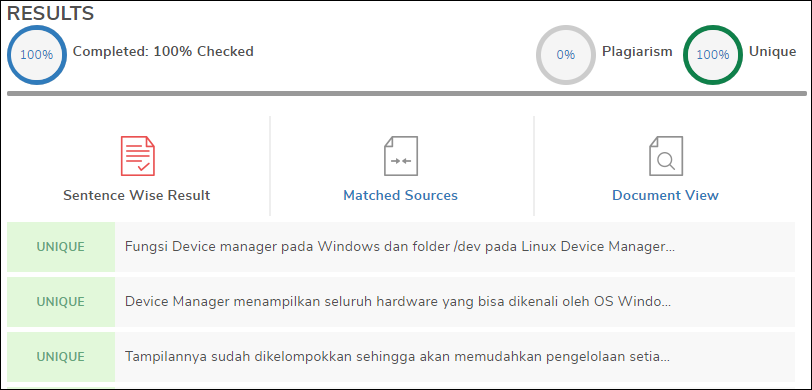
\includegraphics[width=0.5\textwidth]{figures/chapter5/1164074/1}
	\caption{Check Plagiarisme}
	\label{fig1}
\end{figure}

\section {Kevin Natanae Nainggolan 1174059}
	\begin {enumerate}
		\item  Apa itu fungsi device manager di windows dan folder /dev di linux
			\lstinputlisting [firstline=9, lastline=14]{src/chapter5/teori/1174059.py}
		\item Jelaskan langkah-langkah instalasi driver dari arduino
			\lstinputlisting [firstline=17, lastline=28]{src/chapter5/teori/1174059.py}
		\item Jelaskan bagaimana cara membaca baudrate dan port dari komputer yang sudah terinstall driver
			\lstinputlisting [firstline=31, lastline=34]{src/chapter5/teori/1174059.py}
		\item Jelaskan sejarah library pyserial
			\lstinputlisting [firstline=37, lastline=40]{src/chapter5/teori/1174059.py}
		\item Jelaskan fungsi-fungsi apa saja yang dipakai dari library pyserial
			\lstinputlisting [firstline=43, lastline=46]{src/chapter5/teori/1174059.py}
		\item Jelaskan kenapa butuh perulangan dalam tidak butuh perulangan dalam membaca serial
			\lstinputlisting [firstline=49, lastline=53]{src/chapter5/teori/1174059.py}
		\item Jelaskan bagaimana cara membuat fungsi yang mengunakan pyserial
			\lstinputlisting [firstline=56, lastline=59]{src/chapter5/teori/1174059.py}
	\end {enumerate}

\section{Yusniar Nur Syarif Sidiq / 1164089}
\subsection{Pemahaman Teori}
\begin{enumerate}

\item Apa itu fungsi device manager di windows dan folder /dev di linux?
	\subitem Device manager merupakan perangkat lunak untuk menampilkan seluruh perangkat keras yang di-inisialisasi atau dikenali oleh sistem operasi Windows. Device Manager membantu dalam mengelola atau memange semua perangkat keras yang terpasang dan terdeteksi dalam sistem Windows. Fungsi device manager yaitu menunjukkan informasi detail mengenai suatu hardware, mengelola driver hardware, menaktifkan dan nonaktifkan hardware, dan memberikan terjadinya masalah pada hardware. Folder /dev merupakan representasi dari drive yang terhubung ke sistem operasi Libux dan sistem akan menganggap sebagai file-file direktori.

\item Jelaskan Langkah-langkah instalasi driver arduino
	\begin{itemize}

	\item Install terlebih dahulu Arduino IDE pada PC anda

	\item Pasangkan port USB Arduino Uno pada ports USB PC anda, figure \ref{YNC5-1}
	
	\begin{figure}[!htbp]
		\centerline{\includegraphics[width=0.5\textwidth]{figures/chapter5/1164089/YNC5-1.png}}
		\caption{Memasang Port USB.}
		\label{YNC5-1}
	\end{figure}	

	\item Bula Start dan cari Device Manager, figure \ref{YNC5-2}

	\begin{figure}[!htbp]
		\centerline{\includegraphics[width=0.5\textwidth]{figures/chapter5/1164089/YNC5-2.png}}
		\caption{Mencari Device Manager.}
		\label{YNC5-2}
	\end{figure}	

	\item Carilah Unknown Device yang berbeda di Other Device, figue \ref{YNC5-3}

	\begin{figure}[!htbp]
		\centerline{\includegraphics[width=0.5\textwidth]{figures/chapter5/1164089/YNC5-3.png}}
		\caption{Unknown Device.}
		\label{YNC5-3}
	\end{figure}	

	\item Klik kanan lalu pilih Update Driver Software, figure \ref{YNC5-4}

	\begin{figure}[!htbp]
		\centerline{\includegraphics[width=0.5\textwidth]{figures/chapter5/1164089/YNC5-4.png}}
		\caption{Update Driver Software.}
		\label{YNC5-4}
	\end{figure}	

	\item Akan muncul windows baru lalu pilih  menu Browse my computer for driver software, figure \ref{YNC5-5}

	\begin{figure}[!htbp]
		\centerline{\includegraphics[width=0.5\textwidth]{figures/chapter5/1164089/YNC5-5.png}}
		\caption{Browse my computer for driver software.}
		\label{YNC5-5}
	\end{figure}	

	\item Cari folder Arduino lalu klik next, dan windows akan mencari, figure \ref{YNC5-6}

	\begin{figure}[!htbp]
		\centerline{\includegraphics[width=0.5\textwidth]{figures/chapter5/1164089/YNC5-6.png}}
		\caption{Open Folder Arduino.}
		\label{YNC5-6}
	\end{figure}	

	\item Lalu klik install, figure \ref{YNC5-7}

	\begin{figure}[!htbp]
		\centerline{\includegraphics[width=0.5\textwidth]{figures/chapter5/1164089/YNC5-7.png}}
		\caption{Install.}
		\label{YNC5-7}
	\end{figure}	

	\end{itemize}

\item Jelaskan bagaimana cara membaca baudrate dan port dari komputer yang sudah terinstall driver !

	\subitem Cara Membaca Baudrate
	\begin{itemize}
		\item Pertama kita buka Device Manager
		\item Lalu pilih Port (COM \& LPT)
		\item Klik dua kali pada COM yeng telah tersambung
		\item Pilih menu Port Setting dan disitulah kita dapat melihat baudrate
	\end{itemize}

	\subitem Cara Membaca Port
	\begin{itemize}
		\item Pertama kita buka Device Manager
		\item Lalu pilih Port (COM \& LPT)
		\item Dan lihat apabila Arduino sudah tersambung maka akan terbaca
	\end{itemize}

\item Jelaskan sejarah Library pyserial !.
	\subitem PySerial adalah paket Python yang menfasilitasi komunikasi serial antara PC dengan perangkat keras eksternal. PySerial menyediakan antarmuka untuk berkomunikasi melalui protokol komunikasi serial. Komunikasi serial adalah salah satu protokol komunikasi komputer tertua. Protokol komunikasi serial mendahului spesifikasi USB yang digunakan oleh komputer dan perangkat keras lain seperti mouse, keyboard, dan webcam. USB adalah singkatan dari Universal Serial Bus. USB dibangun di atas dan memperluas antarmuka komunikasi serial asli.

\item Jelaskan fungsi-fungsi apa saja yang dipakai pada lib pyserial !
	\subitem Fungsi-fungsi Pada Lib Pyserial
	\begin{itemize}
		\item write(data) berfungsi untuk menulis data melalui port serial
		\item readline() berfungsi untuk membaca string dari port serial
		\item read(size) berfungsi untuk membaca jumlah byte dalam port serial
		\item Serial berfugsi untuk membuka port serial
		\item close() berfungsi untuk menutup port serial
	\end{itemize}

\item Jelaskan kenapa butuh perulangan dan tidak butuh perulangan dalam membaca serial !
	\subitem Karena agar kita mendapatkan data yang cukup banyak supaya semakin akurat maka dari itu kita membutuhkan perulangan dan bila tidak dilakukan perulangan maka data hanya muncul sekali saja.

\item Jelaskan bagaimana cara membuat fungsi yang menggunakan pyserial !

	\subitem Membuat Fungsi Dengan Pyserial

	\lstinputlisting[firstline=1, lastline=9]{src/chapter5/1164089/1164089_Teori.py}

	Apabila di running dalam spyder maka hasilnya akan seperti pada figure \ref{YNC5-8}

	\begin{figure}[!htbp]
		\centerline{\includegraphics[width=0.5\textwidth]{figures/chapter5/1164089/YNC5-8.png}}
		\caption{Fungsi Pyserial.}
		\label{YNC5-8}
	\end{figure}	

Cek Plagiat dapat dilihat pada figire \ref{YNC5-CekPlagiat}

	\begin{figure}[!htbp]
		\centerline{\includegraphics[width=0.5\textwidth]{figures/chapter5/1164089/YNC5-CekPlagiat.png}}
		\caption{Cek Plagiat.}
		\label{YNC5-CekPlagiat}
	\end{figure}		

\end{enumerate}


\chapter{Judul Bagian Keenam}

\section{Fathi Rabbani / 1164074}
\subsection{Teori}
\begin{enumerate}
\item Matplotlib
\par Library yang ada pada pemrograman Python yang berguna untuk membuat data grafik yang berdimensi 2.

\item Membuat Sumbu X dan Y
\par membuat sumbu X dan Y pada penggunaan Library Matplotlib adalah dengan menjelaskan setiap detail data array yang dimiliki sebagai contohnya ada pada Code Berikut : 
\lstinputlisting[firstline=3, lastline=8]{src/chapter6/1164074/code.py}

\item Penggunaan Jenis Plot di Matplotlib
\par ada berbagai macam Jenis PLot yang ada pada Matplotlib, diantaranya adalah :
\begin{itemize}
\item \lstinputlisting[firstline=2, lastline=8, caption=Jenis Garis]{src/chapter6/1164074/code.py}
\item \lstinputlisting[firstline=11, lastline=13, caption=Jenis Titik]{src/chapter6/1164074/code.py}
\item \lstinputlisting[firstline=16, lastline=20, caption=Jenis Batang]{src/chapter6/1164074/code.py}
\item \lstinputlisting[firstline=23, lastline=33, caption=Jenis Pie]{src/chapter6/1164074/code.py}
\end{itemize}

\item Menggunakan Legend dan Label
\par Legend pada matplotlib digunakan untuk menunjukan penggunaan grafik yang ditampilkan. contohnya dapat dilihat pada code berikut : 
\lstinputlisting[firstline=36, lastline=38, caption=Code penggunaan Legend pada Matplotlib]{src/chapter6/1164074/code.py}

\par Label pada matplotlib digunakan untuk menambahkan data Text pada grafik agar mudah untuk dibaca.
\lstinputlisting[firstline=42, lastline=45, caption=Code penggunaan Label pada Matplotlib]{src/chapter6/1164074/code.py}

\item Fungsi subplot di Matplotlib
\par Fungsi yang digunakan untuk menambahkan beberapa diagram sekaligus dalam satu sintaks. contoh code dan penggunaannya dapat dilihat pada Code dan Gambar \ref{data1}
\lstinputlisting[firstline=48, lastline=74, caption= Code penggunaan Subplot pada Matplotlib]{src/chapter6/1164074/code.py}
\begin{figure} [!htbp]
	\centerline{\includegraphics[width=0.5\textwidth]{figures/chapter6/1164074/1}}
	\caption{Penggunaan Subplot pada Matplotlib}
	\label{data1}
\end{figure}

\item Parameter Color
\par Penggunaan warna memiliki peran penting dalam membuat tampilan Grafik lebih menarik dan tidak membosankan, berikut ini adalah daftar penggunaan warna pada Matplotlib :

\begin{itemize}
	\item b : Untuk memberikan warna biru
	\item g : Untuk memberikan warna hijau
	\item r : Untuk memberikan warna merah
	\item c : Untuk memberikan warna biru muda
	\item m : Untuk memberikan warna pink
	\item y : Untuk memberikan warna kuning
	\item k : Untuk memberikan warna hitam
	\item w : Untuk memberikan warna putih
\end{itemize}


\item Cara kerja Fungsi hist
\par Fungsi Hist merupakan fungsi yang berguna untuk membuat data grafik Batang yang memiliki nilai banyak (Array). contoh Code dan penjelasanya dapat dilihat pada Gambar \ref{data2}
\lstinputlisting[firstline=77, lastline=81, caption= Code penggunaan Subplot pada Matplotlib]{src/chapter6/1164074/code.py}
\begin{figure} [!htbp]
	\centerline{\includegraphics[width=0.5\textwidth]{figures/chapter6/1164074/2}}
	\caption{Hasil dari Penggunaan Hist dari Code tersebut}
	\label{data2}
\end{figure}

\item Keterangan Lebih tentang Parameter pada Fungsi Pie
\begin{itemize}
\item Labels
\par Isi dengan tipe data list dan tidak wajib untuk digunakan. Fungsi parameter labels untuk memberi label pada setiap pecahan data yang ada pada grafik pie yang ditampilkan.

\item Colors
\par Tipe data array atau sejenis dan tidak wajib untuk digunakan. Fungsi parameter colors untuk mengganti warna pada setiap pecahan yang ada. Jika tidak digunakan atau ditentukan, maka warna yang akan dipakai adalah warna yang aktif atau standar.
	
\item Startangle
\par Tipe data pecahan atau float, tidak wajib untuk digunakan. Fungsi parameter startangle adalah fungsi untuk memutar grafik agar berubah posisi dengan acuan yaitu angle awalan dari grafik pie.

	
\item Shadow
\par Bertipe data boolean dan tidak wajib digunakan. Fungsi parameter shadow digunakan untuk membuat bayangan pada bawah grafik pie yang ditampilkan. 
	
\item Explode
\par Bertipe data array atau sejenis dan tidak wajib digunakan. Fungsi parameter explode adalah menentukan radius untuk mengimbangi setiap pecahan pada grafik pie. Jika radius lebih dari 0 maka pecahan akan mulai menjauh dari pusat dan terlihat seperti keluar dari grafik lingkaran tersebut.

\item Autopct
\par Bertipe data string atau fungsi dan tidak wajib digunakan. Fungsi parameter autopct adalah memberi label pada irisan dengan labelnya berupa fungsi atau string. 
\end{itemize}

\item Check Plagiarisme

\begin{figure} [!htbp]
	\centerline{\includegraphics[width=0.5\textwidth]{figures/chapter6/1164074/3}}
	\caption{Hasil Check Data Plagiarisme}
	\label{data3}
\end{figure}
\end{enumerate}

\section{Yusniar Nur Syarif Sidiq / 1164089}
\subsection{Pemahaman Teori}

\begin{enumerate}

\item Apa itu fungsi library matplotlib ?
	\subitem Library Matplotllib adalah library python dengan 2D yang dapat menghasilkan plot dengan kualitas yang cukup tinggi dalam berbagai format dan dapat digunakan di beberbagai macam platform. Fungsi dari Library Matplotlib ini yaitu membuat grafik dalam berbagai bentuk seperti grafik diagram batang, berbentuk garis, lingkaran, histogram, dan lain sebagainya.

\item Jelaskan langkah - langkah membuat sumbu X dan Y di matplotlib !

	\begin{itemize}
		\item Lakukan Import Library Matplotlib terlebih dahulu dengan source code seperti berikut,
			\lstinputlisting [firstline=1, lastline=2]{src/chapter6/1164089/1164089.py}
		\item Buatlah dua variabel yang dapat menampung nilai dengan source code seperti berikut,
			\lstinputlisting [firstline=6, lastline=7]{src/chapter6/1164089/1164089.py}
		\item Panggil variabel tersebut dengan fungsi plot seperti source code berikut ini,
			\lstinputlisting [firstline=9, lastline=9]{src/chapter6/1164089/1164089.py}
		\item Untuk menamilkan hasilnya gunakan show seperti source code berikut ini,
			\lstinputlisting [firstline=11, lastline=11]{src/chapter6/1164089/1164089.py}
		\item Sehingga hasilnya dapat kita lihat di figure \ref{YNC6-1}
	\end{itemize}

	\begin{figure}[!htbp!]
		\centerline{\includegraphics[width=0.5\textwidth]{figures/chapter6/1164089/YNC6-1.png}}
		\caption{Hasil Melakukan Plot Sumbu X dan Y.}
		\label{YNC6-1}
	\end{figure}

\item Jelaskan bagaimana perbedaan fungsi dan cara pakai untuk berbagai jesnis (bar, histogram, scatter, dll) jenis plot di matplotlib !

	\begin{itemize}

		\item Diagram Batang atau Bar Graphic dimana fungsi ini akan melakukan plot dan menampilkannya dengan bentuk diagram 			         batang, untuk membuat source codenya perhatikan dibawah dan hasilnya akan ditampilkan pada figure \ref{YNC6-1}.
		         \lstinputlisting [firstline=15, lastline=27]{src/chapter6/1164089/1164089.py}

			\begin{figure}[!htbp!]
				\centerline{\includegraphics[width=0.5\textwidth]{figures/chapter6/1164089/YNC6-2.png}}
				\caption{Fungsi Bar.}
				\label{YNC6-2}
			\end{figure}

		\item Histogram, dimana pada fungsi ini akan melakukan plot penggabungan data yang telah dikelompokkan, untuk 				         membuatnya perhatikan source code dibawah dan hasilnya akan ditampilkan pada figure \ref{YNC6-3}.
		         \lstinputlisting [firstline=31, lastline=39]{src/chapter6/1164089/1164089.py}

			\begin{figure}[!htbp!]
				\centerline{\includegraphics[width=0.5\textwidth]{figures/chapter6/1164089/YNC6-3.png}}
				\caption{Fungsi Histogram.}
				\label{YNC6-3}
			\end{figure}

		\item Scatter Plot, dimana fungsi ini akan melakukan plot berbentuk titik-titik yang masing-masing memiliki nilai variabel, 				         untuk membuatnya perhatikan source code dibawah dan hasilnya akan ditampilkan pada figure \ref{YNC-4}.
		        \lstinputlisting [firstline=43, lastline=56]{src/chapter6/1164089/1164089.py}

		        \begin{figure}[!htbp!]
				\centerline{\includegraphics[width=0.5\textwidth]{figures/chapter6/1164089/YNC6-4.png}}
				\caption{Fungsi Scatter Plot.}
				\label{YNC6-4}
			\end{figure}

		\item Area Plot, dimana fungsi ini akan melakukan pelacakan terhadap perubahan antar dua kelompok atau lebih yang 				         terkait satu kategori secara keseluruhan, untuk membuatnya perhatikan source code dibawah dan hasilnya akan 				         ditampilkan pada figure \ref{YNC6-5}.
		        \lstinputlisting [firstline=60, lastline=79]{src/chapter6/1164089/1164089.py}

		         \begin{figure}[!htbp!]
				\centerline{\includegraphics[width=0.5\textwidth]{figures/chapter6/1164089/YNC6-5.png}}
				\caption{Fungsi Area Plot.}
				\label{YNC6-5}
			\end{figure}

		\item Pie Plot, dimana pada fungsi ini akan digunakan dalam menunjukkan presentase yang mewakili setiap kategori, untuk 			         membuatnya perhatikan source code dibawah dan hasilnya akan ditampilkan pada figure \ref{YNC6-6}.
		         \lstinputlisting [firstline=83, lastline=104]{src/chapter6/1164089/1164089.py}

		         \begin{figure}[!htbp!]
				\centerline{\includegraphics[width=0.5\textwidth]{figures/chapter6/1164089/YNC6-6.png}}
				\caption{Fungsi Pie Plot.}
				\label{YNC6-6}
			\end{figure}

		\item Line Graphic, dimana fungsi ini akan melakukan plot dengan bentuk line, untuk membuatnya perhatikan source code 			         dibawah dan hasilnya akan ditampilkan pada figure \ref{YNC6-7}.
		         \lstinputlisting [firstline=108, lastline=116]{src/chapter6/1164089/1164089.py}

		         \begin{figure}[!htbp!]
				\centerline{\includegraphics[width=0.5\textwidth]{figures/chapter6/1164089/YNC6-7.png}}
				\caption{Fungsi Line Graphic.}
				\label{YNC6-7}
			\end{figure}

	\end{itemize}

\item Jelaskan bagaimana cara menggunakan legend dan label serta kaitannya fungsi tersebut !
	
	\begin{itemize}

		\item Pertama kita akan membuat 4 variabel terlebih dahulu, perhatikan source code berikut,
		         \lstinputlisting [firstline=120, lastline=125]{src/chapter6/1164089/1164089.py}

		\item Dalam membuat fungsi legend kita akan mendefinisikan parameter label pada fungsi plot, dimana parameter label ini 			         akan digunakan untuk memberikan keterangan pada tiap line, perhatikan source code dibawah ini,
		         \lstinputlisting [firstline=126, lastline=127]{src/chapter6/1164089/1164089.py}

		\item Selanjutnya kita akan memberikan title dan nama pada setiap sumbu, gunakan source code seperti berikut,
		         \lstinputlisting [firstline=128, lastline=130]{src/chapter6/1164089/1164089.py}

		\item Panggil fungsi legend dan tampilkan di console gunakan source code berikut,
		         \lstinputlisting [firstline=131, lastline=133]{src/chapter6/1164089/1164089.py}

		\item Hasilnya dapat kita lihat pada figure \ref{YNC6-8}

	\end{itemize}

		\begin{figure}[!htbp!]
			\centerline{\includegraphics[width=0.5\textwidth]{figures/chapter6/1164089/YNC6-8.png}}
			\caption{Fungsi Legend Dan Label.}
			\label{YNC6-8}
		\end{figure}

\item Jelaskan apa fungsi dari subplot di matplotlib, dan bagaimana cara kerja dari fungsi subplot, sertakan ilustrasi dan gambar sendiri dan apa parameternya jika ingin menggambarkan plot dengan 9 subplot di dalamnya !
	\subitem Fungsi Subplot digunakan untuk membuat plot di dalam satu gambar, dimana fungsi subplot memiliki parameter pertama akan menentukan kolomnya, dan pada parameter kedua akan menentukan jumlah barisnya, dan parameter ketiga akan menentukan index plotnya, untuk membuatnta perhatikan source code dibawah dan hasilnya akan ditampilkan pada figure \ref{YNC6-9}.
	\lstinputlisting [firstline=137, lastline=149]{src/chapter6/1164089/1164089.py}

		\begin{figure}[!htbp!]
			\centerline{\includegraphics[width=0.5\textwidth]{figures/chapter6/1164089/YNC6-9.png}}
			\caption{Fungsi Subplot.}
			\label{YNC6-9}
		\end{figure}

\item Sebutkan semua parameter color yang bisa digunakan (contoh: m,c,r,k,...dkk) !
	\subitem Ada beberapa parameter warna yang dapat kita gunakan pada library matplotlib ini yaitu :
	\begin{itemize}
		\item r menunjukkan arti red
		\item b menunjukkan arti blue
		\item g menunjukkan arti green
		\item c menunjukkan arti cyan
		\item y menunjukkan arti yellow
		\item m menunjukkan arti magenta
		\item k menunjukkan arti black
		\item w menunjukkan arti white
	\end{itemize}

\item Jelaskan bagaimana cara kerja dari fungsi hist, sertakan ilustrasi dan gambar sendiri !
	\subitem Cara kerja dari fungsi hist atau biasa kita sebut dengan histogram, dimana akan melakukan eksekusi terhadap data yang telah dikelompokkan dan akan ditampilkan perhitungan jumlah data yang keluar, misalnya saya akan memprediksi jumlah angka yang akan keluar ada berapa, maka dibutuhkan lah source code seperti berikut,
	\lstinputlisting [firstline=31, lastline=39]{src/chapter6/1164089/1164089.py}
Hasil dari source code tersebut akan diperlihatkan pada figure \ref{YNC6-10}.

		\begin{figure}[!htbp!]
			\centerline{\includegraphics[width=0.5\textwidth]{figures/chapter6/1164089/YNC6-10.png}}
			\caption{Fungsi Subplot.}
			\label{YNC6-10}
		\end{figure}

\item Jelaskan lebih mendalam tentang parameter dari fungsi pie diantarannya labels, colors, startangle, shadow, explode, autopct !

	\begin{itemize}
		\item Labels digunakan untuk memberikan keterangan pada tiap presentase
		\item Colors digunakan untuk memberikan warna pada tiap presentase agar terlihat berbeda-beda
		\item Startangle digunakan untuk memutar plot dengan derajat yang telah ditentukan
		\item Shadow digunakan untuk memberikan efek bayangan pada plot
		\item Explode digunakan untuk memisahkan tiap potongan pie pada plot
		\item Autopct digunakan untuk menentukan jumlah angka dibelakang koma
	\end{itemize}

\end{enumerate}

\subsection{Keterampilan Pemrograman}
\begin{enumerate}

\item Buatlah Library Fungsi dengan nama NPM\_bar.py untuk plot dengan jumlah subplot adalah NPM mod 3 + 2 !
	\lstinputlisting [firstline=1, lastline=20]{src/chapter6/1164089/1164089_bar.py}
	\subitem Hasil dari source code tersebut akan menampilkan 4 biji bar, dikarenakan figure yang terlalu besar saya sceenshoot 				    seperti pada figure \ref{YNC6-11}.

	\begin{figure}[!htbp!]
		\centerline{\includegraphics[width=0.5\textwidth]{figures/chapter6/1164089/YNC6-11.png}}
		\caption{Fungsi Bar Praktikum.}
		\label{YNC6-11}
	\end{figure}

\item Buatlah Library Fungsi dengan nama NPM\_scatter.py untuk plot dengan jumlah subplot NPM mod 3 + 2 !
	\lstinputlisting [firstline=1, lastline=22]{src/chapter6/1164089/1164089_scatter.py}
	\subitem Pada source code tersebut dapat dilihat pada figure \ref{YNC6-12}.

	\begin{figure}[!htbp!]
		\centerline{\includegraphics[width=0.5\textwidth]{figures/chapter6/1164089/YNC6-12.png}}
		\caption{Fungsi Scatter Praktikum.}
		\label{YNC6-12}
	\end{figure}

\item Buatlah Library Fungsi dengan nama NPM\_pie.py untuk plot dengan jumlah subplot NPM mod 3 + 2 !
	\lstinputlisting [firstline=1, lastline=22]{src/chapter6/1164089/1164089_pie.py}
	\subitem Pada source code tersebut dapat dilihat pada figure \ref{YNC6-13}.

	\begin{figure}[!htbp!]
		\centerline{\includegraphics[width=0.5\textwidth]{figures/chapter6/1164089/YNC6-13.png}}
		\caption{Fungsi Pie Praktikum.}
		\label{YNC6-13}
	\end{figure}

\item Buatlah Library Fungsi dengan nama NPM\_plot.py untuk plot dengan jumlah subplot NPM mod 3 + 2 !
	\lstinputlisting [firstline=1, lastline=22]{src/chapter6/1164089/1164089_plot.py}
	\subitem Pada source code tersebut dapat dilihat pada figure \ref{YNC6-14}.

	\begin{figure}[!htbp!]
		\centerline{\includegraphics[width=0.5\textwidth]{figures/chapter6/1164089/YNC6-14.png}}
		\caption{Fungsi Plot Praktikum.}
		\label{YNC6-14}
	\end{figure}

\end{enumerate}

\subsection{Keterampilan Penanganan Error}

\begin{enumerate}

\item Error yang saya dapatkan terlihat pada figure \ref{YNC6-15} yang merupakan NameError dikarenakan variabel yang saya deklarasikan tidak sesuai, cara membenarkannya kita ganti variabel tersebut menjadi x dan y, dan untuk membuat fungsi try exceptnya dapat perhatikan source code berikut ini,

	\lstinputlisting [firstline=177, lastline=187]{src/chapter6/1164089/1164089.py}

	\begin{figure}[!htbp!]
		\centerline{\includegraphics[width=0.5\textwidth]{figures/chapter6/1164089/YNC6-15.png}}
		\caption{Error Yang Di Dapat.}
		\label{YNC6-15}
	\end{figure}

\end{enumerate}

\section {Kevin Natanae Nainggolan 1174059}
	\subsection {TEORI}
	\begin {enumerate}
		\item  Apa itu fungsi library matplotlib
			\newline Library plotting 2 dimensi Python yang menciptakan gambar publikasi bermutu di dalam berbagai macam format hardcopy
		\item Jelaskan langkah-langkah membuat sumbu X dan Y di matplotlib
			\newline  Membuat sumbu x dan y pada matplotlib, kita bisa membuatnya menggunakan list untuk mempermudah penyimpanan nilai setiap sumbunya. Seperti kode di bawah
			\lstinputlisting [firstline=2, lastline=5]{src/chapter6/teori/1174059.py}
		\item Jelaskan bagaimana perbedaan fungsi dan cara pakai untuk berbagai jenis(bar,histogram,scatter,line dll) jenis plot di matplotlib
			\newline Untuk membedakan fungsi plot yang digunakan adalah dengan melihat bentuk grafik yang akan di tampilkan sesuai dengan perintah yang digunakan pada pemogramannya, dan untuk cara pengguna plot tersebut bisa dilihat sebagai berikut
			\lstinputlisting [firstline=2, lastline=2]{src/chapter6/teori/1174059.py}
				\begin {enumerate}
					\item bar 
					\newline Perhatikan kode dalam membentuk diagram bar seperti berikut
						\lstinputlisting [firstline=21, lastline=29]{src/chapter6/teori/1174059.py}
					\item histogram
					\newline Dalam penggunaanya plot bar x dan y dapat diatur dengan angka koma
						\lstinputlisting [firstline=35, lastline=41]{src/chapter6/teori/1174059.py}
					\item scatter
					\newline Diagram yang penampilannya dengan titik titik sebagai penandanya
						\lstinputlisting [firstline=46, lastline=56]{src/chapter6/teori/1174059.py}
					\item line
					\newline Perhatikan kode dalam membentuk diagram line seperti berikut
						\lstinputlisting [firstline=13, lastline=16]{src/chapter6/teori/1174059.py}
					\item stack plot
					\newline Penggunaan stack plot ini seperti diagram line, dengan warna yang mengisinua, serta antar line itu bisa berdekatan. Berikut Contoh penggunaannya
						\lstinputlisting [firstline=61, lastline=83]{src/chapter6/teori/1174059.py}
				\end {enumerate}
		\item Jelaskan bagaimana cara menggunakan legend dan label serta kaitannya dengan fungsi tersebut
		\newline Penggunaan legend untuk memudahkan dalam membaca grafik. Dalam penggunaan lagend dan label perhatikan code berikut
			\lstinputlisting [firstline=55, lastline=55]{src/chapter6/teori/1174059.py}
		\item Jelaskan apa fungsi dari subplot di matplotlib, dan bagaimana cara kerja dari fungsi subplot, sertakan ilustrasi dan gambar sendiri dan apa parameternya jika ingin menggambar plot dengan 9 subplot di dalamnya
		\newline fungsi dari subplot dari matplotlib untuk bisa membuat lebih dari 1 grafik dalam sebuah program. Untuk parameternya sendiri kami menggunakan t1 dan t2. Cara kerjanya sendiri bisa d cek sebagai berikut
			\lstinputlisting [firstline=87, lastline=112]{src/chapter6/teori/1174059.py}
		\item Sebutkan semua parameter color yang bisa digunakan (contoh: m,c,r,k,... dkk)
			\begin {itemize}
				\item R untuk warna Red atau Merah
				\item G untuk warna Green atau Hijau
				\item B untuk warna Blue atau Biru
				\item C untuk warna Cyan atau Biru Muda
				\item M untuk warna Mangenta atau Merah Tua
				\item Y untuk warna Yellow Atau Kuning
				\item K untuk warna blacK atau Hitam
			\end {itemize}
		\item Jelaskan bagaimana cara kerja dari fungsi hist, sertakan ilustrasi dan gambar sendiri
		\newline  Fungsi hist digunakan untuk menjumlahkan beberapa data yang memenuhi kriteria pramater yang kita tentukan, seprti contoh kode dibawah
			\lstinputlisting [firstline=116, lastline=121]{src/chapter6/teori/1174059.py}
		\item Jelaskan lebih mendalam tentang parameter dari fungsi pie diantaranya labels, colors, startangle, shadow, explode, autopct
			\newline  
			\begin{itemize}
	\item labels : Isi dengan tipe data list dan tidak wajib untuk digunakan. Fungsi parameter labels untuk memberi label pada setiap pecahan data yang ada pada grafik pie yang ditampilkan.
	\item colors : Tipe data array atau sejenis dan tidak wajib untuk digunakan. Fungsi parameter colors untuk mengganti warna pada setiap pecahan yang ada. Jika tidak digunakan atau ditentukan, maka warna yang akan dipakai adalah warna yang aktif atau standar.
	\item startangle : Tipe data pecahan atau float, tidak wajib untuk digunakan. Fungsi parameter startangle adalah fungsi untuk memutar grafik agar berubah posisi dengan acuan yaitu angle awalan dari grafik pie.
	\item shadow : Bertipe data boolean dan tidak wajib digunakan. Fungsi parameter shadow digunakan untuk membuat bayangan pada bawah grafik pie yang ditampilkan. 
	\item explode : Bertipe data array atau sejenis dan tidak wajib digunakan. Fungsi parameter explode adalah menentukan radius untuk mengimbangi setiap pecahan pada grafik pie. Jika radius lebih dari 0 maka pecahan akan mulai menjauh dari pusat dan terlihat seperti keluar dari grafik lingkaran tersebut.
	\item autopct : Bertipe data string atau fungsi dan tidak wajib digunakan. Fungsi parameter autopct adalah memberi label pada irisan dengan labelnya berupa fungsi atau string. 
			\end{itemize}
	\end {enumerate}
	
		\subsection {PRAKTEK}
		\begin {enumerate}
			\item Buatlah librari fungsi (file terpisah/library dengan nama NPM bar.py) untuk plot dengan jumlah subplot adalah NPM mod 3 + 2
				\lstinputlisting [firstline=8, lastline=27]{src/chapter6/praktek/1174059/chap6_1174059_bar.py}
			\item Buatlah librari fungsi (file terpisah/library dengan nama NPM scatter.py) untuk plot dengan jumlah subplot NPM mod 3 + 2
				\lstinputlisting [firstline=8, lastline=38]{src/chapter6/praktek/1174059/chap6_1174059_pie.py}
			\item Buatlah librari fungsi (file terpisah/library dengan nama NPM pie.py) untuk plot dengan jumlah subplot NPM mod 3 + 2
				\lstinputlisting [firstline=8, lastline=27]{src/chapter6/praktek/1174059/chap6_1174059_scater.py}
			\item Buatlah librari fungsi (file terpisah/library dengan nama NPM plot.py) untuk plot dengan jumlah subplot NPM mod 3 + 2
				\lstinputlisting [firstline=8, lastline=27]{src/chapter6/praktek/1174059/chap6_1174059_plot.py}
		\end {enumerate}
		
	\subsection {PENANGANAN EROR}
		\par Tuliskan peringatan error yang didapat dari mengerjakan praktek ketiga ini, dan jelaskan cara penanganan error tersebut. dan Buatlah satu fungsi yang menggunakan gunakan try except untuk menanggulangi error tersebut
		\lstinputlisting [firstline=8, lastline=30]{src/chapter6/teori/1174059/chap6_1174059_penanganan.py

\bibliographystyle{IEEEtran} 
%\def\bibfont{\normalsize}
\bibliography{references}


%%%%%%%%%%%%%%%
%%  The default LaTeX Index
%%  Don't need to add any commands before \begin{document}
\printindex

%%%% Making an index
%% 
%% 1. Make index entries, don't leave any spaces so that they
%% will be sorted correctly.
%% 
%% \index{term}
%% \index{term!subterm}
%% \index{term!subterm!subsubterm}
%% 
%% 2. Run LaTeX several times to produce <filename>.idx
%% 
%% 3. On command line, type  makeindx <filename> which
%% will produce <filename>.ind 
%% 
%% 4. Type \printindex to make the index appear in your book.
%% 
%% 5. If you would like to edit <filename>.ind 
%% you may do so. See docs.pdf for more information.
%% 
%%%%%%%%%%%%%%%%%%%%%%%%%%%%%%

%%%%%%%%%%%%%% Making Multiple Indices %%%%%%%%%%%%%%%%
%% 1. 
%% \usepackage{multind}
%% \makeindex{book}
%% \makeindex{authors}
%% \begin{document}
%% 
%% 2.
%% % add index terms to your book, ie,
%% \index{book}{A term to go to the topic index}
%% \index{authors}{Put this author in the author index}
%% 
%% \index{book}{Cows}
%% \index{book}{Cows!Jersey}
%% \index{book}{Cows!Jersey!Brown}
%% 
%% \index{author}{Douglas Adams}
%% \index{author}{Boethius}
%% \index{author}{Mark Twain}
%% 
%% 3. On command line type 
%% makeindex topic 
%% makeindex authors
%% 
%% 4.
%% this is a Wiley command to make the indices print:
%% \multiprintindex{book}{Topic index}
%% \multiprintindex{authors}{Author index}

\end{document}
